\documentclass[	11pt,		% 11 Punkte hohe Schrift
				a4paper,	% Einstellung des Ausdrucks auf DIN A4
				fleqn,		% linksbündige, abgesetzte Formeln
				reqno,		% rechts stehende Formelnummer
				BCOR12mm,	% Bindekorrektur von 12mm
				chapterprefix=false,	% Ausgabe von Kapitel: 
				appendixprefix=true, % Überschrift im Anhang X und dann neue Zeile und Titel
				parskip=half,
				DIV=calc,
				final,		% Abgabe Version
]{scrartcl}
%\usepackage{natbib}
\usepackage{packages}
\usepackage{layout}
\usepackage{hyperref}
\usepackage[ngerman,bookmarks=true,bookmarksopen=true,bookmarksnumbered=true]{hyperref}
\usepackage{listingsutf8}
\usepackage{caption}
\graphicspath{{image/}}
\DeclareGraphicsExtensions{.png,.pdf}

\bibliography{src/literatur}	% Literaturverzeichnis

\newtheorem{defi}{Definition}
\newtheorem{bsp}{Beispiel}
\newtheorem{satz}{Satz}
\newtheorem{theo}{Theorem}

\newcommand{\bspautorefname}{Beispiel}
\newcommand{\defiautorefname}[1]{Definition #1}
\newcommand{\theoautorefname}{Theorem}

\newcommand{\RM}[1]{\MakeUppercase{\romannumeral #1{}}} 

\setcounter{tocdepth}{4}
\setcounter{secnumdepth}{4} 
\lstset{inputencoding=utf8/latin1}
\lstdefinestyle{customc}{
  belowcaptionskip=1\baselineskip,
  breaklines=true,
  linewidth=1\textwidth,
  %frame=L,
  xleftmargin=\parindent,
  language=C,
  numbers=left,
  tabsize=3, 
  showstringspaces=false,
  basicstyle=\footnotesize\ttfamily,
  keywordstyle=\bfseries\color{green!40!black},
  morekeywords={uint8_t,uint16_t,int8_t,PROCESS,PROCESS_THREAD, PROCESS_BEGIN, PROCESS_END, AUTOSTART_PROCESSES},
  commentstyle=\itshape\color{purple!40!black},
  identifierstyle=\color{blue},
  stringstyle=\color{orange},
}

\DeclareCaptionFont{white}{ \color{white} }
\DeclareCaptionFormat{listing}{
  \colorbox[cmyk]{0.43, 0.35, 0.35,0.01 }{
    \parbox{\textwidth}{\hspace{15pt}#1#2#3}
  }
}
%\captionsetup[lstlisting]{ format=listing, labelfont=white, textfont=white, singlelinecheck=false, margin=0pt, font={bf,footnotesize} }

\begin{document}
	% Cover
	\begin{titlepage}
  \begin{centering}
  \begin{figure}[h!]
    \centering
    
\includegraphics[width=310pt]{UniLogo}
  \end{figure}

  \vspace*{-0.8cm}

  \begin{figure}[h!]
    \centering
    
\includegraphics[width=280pt]{BUIENGLOGO}
  \end{figure}

  \vspace*{0.4cm}
  
  \textsf{\Huge \textbf{Projektgruppe FAISE\\}}

  \vspace*{0.5cm}
  \noindent Endbericht\\
  im Rahmen des Masterstudiums

  \end{centering}
  
  \vspace*{1.5cm}
  \begin{tabbing}
  xxxxxxxxxxxxxxxx\= \kill
  
  \small Betreuer: \>Prof. Dr.-Ing. Jürgen Sauer\\
  \small \>Dipl.-Ing. (FH) Arne Stasch\\
  \small \>Dipl.-Inform. Jan-Hinrich Kämper\\
  \small \>Prof. Dr.-Ing. Axel Hahn\\\\

  \small Vorgelegt von: \>Berthe Pulcherie Ongnomo\\
  \small \>Chancelle Merveille Tematio Yme\\
  \small \>Christopher Schwarz\\
  \small \>Jan Paul Vox\\
  \small \>Jan-Gerd Meß\\
  \small \>Jannik Fleßner\\
  \small \>Malte Falk\\
  \small \>Mathias Aden\\
  \small \>Michael Goldenstein\\
  \small \>Nagihan Aydin\\
  \small \>Raschid Alkhatib\\
  \small \>Simon Jakubowski\\\\

  \small Abgabetermin:\> 30. September 2014
  \end{tabbing}
\end{titlepage}
	\pagenumbering{Roman}
	% Abstract
	\include{src/abstract}

	% Table of contents
	\clearpage
\ohead[Inhaltsverzeichnis]{Inhaltsverzeichnis}
\chead[Uni Oldenburg]{Uni Oldenburg}
\ihead[PG FAISE]{PG FAISE}
\setheadtopline{1pt}
\setheadsepline{0.5pt}

\ofoot[Endbericht]{Endbericht}
\cfoot[\pagemark]{\pagemark}
\ifoot[30. September 2014]{30. September 2014}
\setfootsepline{0.5pt}
\setfootbotline{1pt}

\tableofcontents
\clearpage

\ohead[Abbildungsverzeichnis]{Abbildungsverzeichnis}
\chead[Uni Oldenburg]{Uni Oldenburg}
\ihead[PG FAISE]{PG FAISE}
\setheadtopline{1pt}
\setheadsepline{0.5pt}

\ofoot[Endbericht]{Endbericht}
\cfoot[\pagemark]{\pagemark}
\ifoot[30. September 2014]{30. September 2014}
\setfootsepline{0.5pt}
\setfootbotline{1pt}

\listoffigures
%\listoftables
	
	% Chapter 1 Einleitung
	\pagenumbering{arabic}
	\clearpage
	\ohead[Einleitung]{Einleitung}
	\chead[Uni Oldenburg]{Uni Oldenburg}
	\ihead[PG FAISE]{PG FAISE}
	\setheadtopline{1pt}
	\setheadsepline{0.5pt}
	\ofoot[Endbericht]{Endbericht}
	\cfoot[\pagemark]{\pagemark}
	\ifoot[30. September 2014]{30. September 2014}
	\setfootsepline{0.5pt}
	\setfootbotline{1pt}
	\section{Einleitung}
In diesem Kapitel wird ein einführender Überblick über die Projektgruppe Fully Autonomous Intralogistic Swarm Experiments gegeben, die im Rahmen der Masterstudiengänge Informatik und Wirtschaftsinformatik in der Abteilung Systemanalyse und -optimierung der Carl von Ossietzky Universität Oldenburg stattgefunden hat. Das Projekt lief über einen Zeitraum von zwei Semestern: Wintersemester 2013/2014 und Sommersemester 2014.


\subsection{Motivation}
Im Zeitalter der Globalisierung werden hohe Anforderungen an die Leistungsfähigkeit von modernen Intralogistiksystemen gestellt. Neben einem hohen Automatisierungsgrad wird gleichzeitig auch eine möglichst hohe Flexibilität gefordert, da sich Anforderungen im logistischen Umfeld häufig ändern (Vgl.\cite{ieft}).    
\\\\
Stetigförderer bieten die Möglichkeit einen automatisierten Materialfluss einzurichten. Es handelt sich dabei um Transportsysteme, die Güter kontinuierlich und automatisiert entlang eines festgelegten Transportwegs befördern (Vgl.\cite{stf}). Ein solches System könnte beispielsweise ein Netz von Schienen sein. Nachteile dieser Systeme sind insbesondere Unflexibilität und schlechte Skalierbarkeit. Ändern sich Anforderungen in einem Logistiksystem, dann stoßen Stetigförderer schnell an ihre Grenzen. Transportwege sind festgelegt und können nicht ohne einen gewissen Aufwand geändert werden. Auch kann die Anzahl an Gütern, die pro Zeiteinheit befördert werden kann, nicht ohne eine Änderung am Transportnetz maximiert werden.
\\\\
Eine Alternative zu Stetigförderern sind Fahrerlose Transportsysteme (FTS). FTS sind ein Gesamtsystem aus Fahrerlosen Transportfahrzeugen, die Ware automatisiert befördern, und der Infrastruktur, die zum Betrieb der Transporteinheiten notwendig ist (Vgl.\cite{fts}). Fahrerlose Transportsysteme sind wesentlich flexibler als Stetigförderer. Müssen mehr Güter befördert werden, so können zusätzliche Transporteinheiten aktiviert werden. Folglich sind FTS problemlos skalierbar und können schnell auf veränderte Anforderungen in einem Intralogistiksystem eingestellt werden. FTS bieten einen automatisierten Warenfluss bei gleichzeitig hoher Flexibilität und entsprechen somit den Anforderungen, die an moderne Intralogistiksysteme gestellt werden.  
\\\\
%Es bietet sich an ein System zu entwickeln, das basierend auf FTS, einen vollautomatisierten %Warenfluss implementiert, um verschiedene Fragestellungen zu untersuchen. Wie muss ein solches %System aufgebaut sein, welche Kommunikationsabläufe sind zwischen den verschiedenen Akteuren %notwendig, welche Anforderungen werden an Hard- und Software gestellt und wie flexibel ist ein %solches System?  

\subsection{Zielsetzung}
Im Rahmen der Projektgruppe FAISE soll ein System entwickelt werden, das den vollautomatisierten Warenfluss in einem Lager auf Basis von Fahrerlosen Transportsystemen simuliert. Dabei sollen die Transporteinheiten nicht zentral gesteuert werden, sondern dezentral agieren.
Das Gesamtsystem besteht aus zwei Teilsystemen, einem physisch vorhandenem System und einer softwarebasierten Simulation. 
\\\\
Das physische System beinhaltet Rampen, auf denen Ware gelagert werden kann und Fahrerlose Transporteinheiten als Fördermittel. Die Akteure kommunizieren miteinander über ein Sensornetzwerk und werden auf Basis von Mikrocontrollern gesteuert. Ziel ist es den Materialfluss von den Transporteinheiten und Rampen vollständig autonom und ohne dezentrale Steuerung durchzuführen. 
\\\\
Das rein softwarebasierte System soll einen automatisierten Warenfluss, der durch Rampen und Fahrzeuge durchgeführt wird, simulieren. Die Realisierung der Akteure in der Software soll an die Eigenschaften der Akteure aus dem physische System angelehnt sein. Beide Systeme sollen unabhängig voneinander laufen. 

\subsection{Einsatzszenario}\label{Einsatzszenario} 
Das Einsatzszenario besteht aus n fahrerlosen Transporteinheiten in einem Umschlagslager. Zusätzlich sind m Rampen verfügbar an denen Pakete zwischengelagert werden können. Im Gegensatz zu einem herkömmlichen Lager, werden Waren in einem Umschlagslager nur kurzfristig gelagert, um anschließend weitertransportiert zu werden. Es herrscht ein kontinuierlicher Materialfluss. Jedes Paket, das ins Lager gebracht wird, ist eindeutig identifizierbar und wird zu einem definierten Zeitpunkt ins Lager gebracht und wieder abgeholt. Die Rampen im Lager sollen drei unterschiedliche Zwecke erfüllen. Eingangsrampen dienen der Warenannahme, Zwischenrampen der Zwischenlagerung. Pakete werden zum Ausgangslager gebracht und zum Zwecke des Weitertransports dort abgeholt. Auf Basis des Einsatzszenarios wird im Rahmen der Anforderungen ein Ablaufszenario erstellt, das die Interaktionen zwischen den Akteuren beschreibt auf deren Basis eine automatisierte, dezentrale Abwicklung des Materialflusses erfolgen kann.

\subsection{Komponenten}
Das zu entwickelnde System lässt sich grob in die Komponenten physisches System und Simulation unterteilen. Das physisches System wiederum lässt sich noch weiter in die Komponenten Materialfluss und Fahrzeuge aufteilen. Das Gesamtsystem lässt sich somit in drei Komponente aufteilen, die im Folgenden beschrieben werden:

\begin{itemize}
\item Materialfluss: Die Komponente Materialfluss beschreibt die Rampen auf denen Pakete gelagert werden. Die Rampen sollen mithilfe von Sensoren mit anderen Rampen und den fahrerlosen Transporteinheiten kommunizieren können. Durch Aktoren soll es möglich sein, Pakete zum Zwecke des Weitertransports an die Fahrzeuge zu übergeben.
\item Fahrzeuge: Die Fahrzeuge übernehmen den Transport der Pakete und kommunizieren mit den Rampen, um den Transport automatisiert abzuwickeln. Die Fahrzeuge sollen anhand von Start- und Zielpunkten in der Lage sein, selbstständig Pfade zu erstellen und diese abzufahren.
\item Simulation: Die Simulation soll als Softwaresystem realisiert werden, dass es erlaubt Szenarien mit einer bestimmten Anzahl an Rampen und Fahrzeugen zu erstellen. Wie im physischen System, sollen die Rampen und Fahrzeuge einen automatisierten Warenfluss durchführen und die Aktionen sollen visualisiert werden.  
\end{itemize} 

	
	% Chapter 2 Stand der Technik
	\clearpage
	\ohead[Stand der Technik]{Stand der Technik}
	\chead[Uni Oldenburg]{Uni Oldenburg}
	\ihead[PG FAISE]{PG FAISE}
	\setheadtopline{1pt}
	\setheadsepline{0.5pt}
	\ofoot[Endbericht]{Endbericht}
	\cfoot[\pagemark]{\pagemark}
	\ifoot[30. September 2014]{30. September 2014}
	\setfootsepline{0.5pt}
	\setfootbotline{1pt}
	\section{Stand der Technik}
Die Fahrerlosen Transportsysteme und die Materialflusssysteme sind Prozesse der Logistik. In den vergangenen Jahren hat die Verbreitung Fahrerloser Transportsysteme (FTS) stark zugenommen. Beim Einsatz von FTS stellen sich vielfältige Konfigurierungs- und Planungsprobleme, so auch die Einsatzplanung f\"ur die einzelnen Fahrerlosen Transportfahrzeuge. (vgl. Günther; Krüger; Schrecker; 2000, S. 2). Der innerbetriebliche Materialfluss von Industrieunternehmen bietet fahrerlosen Transportsystemen (FTS) zahlreiche Einsatzgebiete: Sie verketten Produktionsprozesse, verknüpfen Fertigungsstationen oder ganze Betriebsbereiche und beschicken Montageplätze. Darüber hinaus dienen sie als mobile Werkbank oder versorgen und entsorgen Lager unterschiedlicher Art. Um die Systemvorteile von Fahrerlosen Transportsystemen und Materialflusssystemen zu optimieren, braucht man ein ma\ss gerechtes Wissen auf Ihr spezifisches Anlagekonzept abzustimmen. Wichtige Kriterien sind allerdings z.~B. die Einbindung der Fahrerlosen Transportsysteme in den gesamtbetrieblichen Materialfluss, die Anpassung an die vorhandenen Steuerungshierarchien und die optimale Auslegung der Technik in Bezug auf Fahrzeugbauart, Lastaufnahmemittel, Energiekonzept, Kommunikation und Leitsystem. (vgl. Werner Swoboda, Industrie Anzeiger). Ziele von Fahrerlosen Transportsystemen und Materialflusssystemen sind Kostensenkung durch Personaleinsparung, Verringerung von Transportsch\"aden, hohe Zuverl\"assigkeit in Vorg\"angen und bessere Materialflussplanung.
Dieses Kapitel wird in drei Teile gegliedert. Der erste Teil wird die Fahrerlosen Transportsysteme bzw die Orientierungs- und die Steuerungssysteme vorstellen und erkl\"aren; der zweite Teil ist eine Darstellung der Materialflusssysteme und ihrer verschiedenen Funktionen und der dritte Teil wird erkl\"aren, wie fahrerlose Transport- und Materialflusssysteme in gro\ss en Firmen wie Volkswagen und BMW Anwendung finden.

\subsection{Fahrerlose Transportsysteme}
Nach dem Verein Deutscher Ingenieure 2510 bestehen FTS im Wesentlichen aus "`einem oder mehreren Fahrerlosen Transportfahrzeugen (FTF), einer Leitsteuerung, Einrichtung zur Standortbestimmung und Lagererfassung, Einrichtungen zur Daten\"ubertragung sowie Infrastruktur und peripheren Einrichtungen"'. In seinem Buch Transport und Lagerlogistik fasst Martin die Definition von VDI 2510 eines FTS zusammen. Er beschreibt ein FTS als mit FTF ausgestattete rechnergesteuerte Materialflussanlagen zum automatischen Transport von G\"utern im innerbetrieblichen Materialfluss. (vgl. Martin H, 2006, S.262f). Bei FTS handelt es sich um flurgebundene F\"ordersysteme mit automatisch gef\"uhrten FTF. Die einzelnen FTF bef\"ordern Ladungstr\"ager zwischen zwei oder mehrere Stationen innerhalb eines Gebietes. Die Fahrzeugsteuerung erfolgt automatisch und rechnergest\"utzt. Der Einsatzbereich von FTS ist generell \"uberwiegend innerbetrieblich ausgerichtet. In diesen Rahmen \"ubernehmen FTS sowohl reine F\"orderaufgaben, wie Verkettung von Fertigungs- und Montageeinrichtungen als auch Aufgaben der Lagerbedienung und Kommissionierung. (vgl. G\"unther; Kr\"uger; Schrecker; 2000, S. 3). Das FTS ist eine Technik, die im Vergleich gegen\"uber Stetigf\"ordersystemen eine hohe Anpassungsf\"ahigkeit an die sich \"andernden Marktsituationen zum Vorteil hat. Daher konzentrieren die Forschungs- und Entwicklungsaktivit\"aten sich heutzutage auf die sog. „Zellul\"aren F\"ordersysteme“, in welchen stetige F\"orderanlagen zur Verkn\"upfung von Logistischen Funktionen durch individuelle, autonom arbeitende FTF ersetzt werden (vgl. Ten Hompel; Heidenblut, 2008). Die Haupteinsatzgebiete des FTS liegen nun in der Intralogistik. Also bei der Organisation, der Steuerung, der Durchf\"uhrung und der Optimierung des innerbetrieblichen Waren- und Materialflusses und Logistik, der Informationsstr\"ome sowie des Warenumschlags in Industrie, Handel und \"offentlichen Einrichtungen. Z.~B. Automobil- und Zulieferindustrie, Papiererzeugung und –verarbeitung, Elektroindustrie, Getr\"anke-, Lebensmittelindustrie, Baustoffe, Stahlindustrie, Kliniklogistik (G\"unter Ullrich, 2011 S. 13). FTS bestehen im Wesentlichen aus drei Systemkomponenten: Die Fahrerlosen Transportfahrzeuge, das Orientierungssystem, das Steuerungssystem. 

\subsection{Fahrerlose Transportfahrzeuge}
Die FTF sind flurgebundene F\"ordermittel mit eigenem Fahrantrieb, die automatisch gef\"uhrt, gesteuert und ber\"uhrungslos gef\"uhrt werden. Sie dienen dem Materialtransport, und zwar zum Ziehen und/oder Tragen von F\"ordergut mit aktiven oder passiven (FTF mit passiver Lastaufnahme werden von anderen F\"ordermitteln gezogen oder manuell mit den G\"utern best\"uckt) Lastaufnahmemittel (VDI 2510). Da das FTS mit Fahrerlosen Aspekten Systematisiert ist, ergibt sich dann aus den funktionalen Ebene Unterschieden zu fahrerbedienten Fahrzeugen, wie z. B. den klassischen Gabelstaplern und FTF: In Rahmen dieser Arbeit wird es nur eine Kategorie von FTF tiefer eingegangen: das Mini-FTF. Die Mini-FTF sind kleine, schnelle, intelligente und flexible Fahrzeuge, die extrem schnell Bed\"urfnisse befriedigen k\"onnen. Heutzutage arbeiten viele Universit\"aten in der ganzen Welt in Swarm bzw. Schw\"arme-Experiment. Hier die kleine FTF sollen intelligent miteinander arbeiten. Die Fahrzeuge sollen sich ohne eine eigene separate FTS-Leitsteuerung untereinander verst\"andigen, Strategien entwickeln und gemeinsam Arbeiten ausf\"uhren. Die Forschungsgebiete hei\"ssen Agentensysteme und Schwarmtheorie. Die Mini-FTF k\"onnen nur intralogistische Aufgaben auff\"ullen. Dennoch sind viele unkonventionelle Einsatzf\"alle denkbar. Die Kommissionierung (eine ausf\"uhrliche Begriffserkl\"arung wird im Teil Materialfluss gegeben) ist die verbreite Anwendungsm\"oglichkeit von Mini-FTF (G\"unter Ullrich, 2011 S. 105).
Als Zusammenfassung kann man sagen, dass die Fahrzeugsteuerung die Systemsicherheit, das Energiemanagement, das Lastaufnahmemittel und die Lenkung eines FTF gew\"ahrleistet. Eine FTF kann ohne Energie nicht funktionieren. Damit ein FTF seine Aufgabe erf\"ullen kann, ist eine Energieversorgung notwendig. Die Energie kann durch Akkus oder Traktionsbatterien oder mit Hilfe eines Induktionssystems oder Stromschiene versorgt werden. Jedoch k\"onnen die beiden Versorgungsarten gekoppelt werden, um einen Hybridsystem zu bekommen. Die Notwendigkeit der Existenz eine Ladestation in einem FTS ist unumstritten. Die FTF m\"ussen immer mit Energie versorgt werden. Je nachdem wie die FTF programmiert sind, kann ein FTF selber zur Ladestation beim Energiebedarf fahren, oder kann ein Auftraggeber (Mensch) es zu Ladestation f\"uhren.

\subsubsection{Orientierungssystem bzw. Navigation}
Das Orientierungssystem bzw. die Navigation dient zur Lokalisierung des Fahrzeugs. Sie ist ein Hilfsmittel zur Berechnung des sichersten Wegs um das Ziel zu erreichen. Au\"sserdem dient die Navigation auch zur Vermeidung von eventuellen Kollisionen. Sie gilt sowohl als f\"ur die Orientierung als auch f\"ur die Sicherheit des Fahrzeuges und sein Umfeld. W\"ahrend seiner Bewegung bzw. Orientierung folgt das FTF einer physischen oder virtuellen Linie (Spur), damit es sein Ziel Gefahrlos erreichen kann. Allerdings aufgrund eines Sicherheitssystems sollte das FTF sofort anhalten, wenn Hindernisse oder Kollisionsgefahr vor ihn stehen. 
Mit Navigationshilfe kennt man nicht nur die Positionierung und Orientierung des Fahrzeuges sondern auch wohin das Fahrzeug gelangen w\"urde, wenn keine auf seine Bewegung ver\"andernden Ma\"ssnahmen ergriffen wurde. Die Steuerung sagt was zu tun ist, und die Navigation bestimmt durch welchen Weg das Fahrzeug dem gew\"unschten Ziel sicher zu erreichen ist bzw. auf einem vorgegebenen Weg zu verfolgen oder eine alternative Weg zu nehmen. Die Steuerung von fahrerlosen Transportfahrzeugen, deren Grundfunktionen und der Umgang mit diesen werden in den VDI- Richtlinien [VDI92], [VDI94], [VDI04] vorgestellt. F\"ur das Konstrukt von fahrerlose Transportsysteme werden verschiedene Ans\"atze verfolgt, die  abh\"angig vom System verschiedene Konstruktionsbem\"uhungen auf das Fahrzeug oder auf der Strecke erfordern. Es gibt mehrere Navigationsverfahren: die physische Leitlinie, die Orientierung durch Magnetmarken, das Global Positioning System (GPS) und die Lasernavigation (vgl. G\"unter Ullrich, 2011 S. 112).
\begin{itemize}
	\item \textbf{Die physische Leitlinie:}  Fahrerlose Transportsysteme, die auf physischen Leitlinien navigieren bzw. fahren, benutzen Einrichtungen am oder im Fu\"ssboden. Die verschiedenen Varianten sind:
 \item \textbf{Orientierung durch optische Leitspur:} Bei dieser Methode wird ein farbstrich mit deutlichem Farbkontrast zum umgebenden Boden entweder lackiert oder mit einem speziellen Gewebeband aufgebracht wird. Eine geeignete Kamerasensorik unter dem Fahrzeug nutzt ebenfalls Kantendetektions-Algorithmen  und errechnet so die Ansteuerungssignale f\"ur den Lenkmotor (G\"unter Ullrich, 2011 S. 112). Optische Verfahren dienen durch eine st\"andige Kurskorrektur eine hohe  Fahrgenauigkeit zu erreichen. 
\item \textbf{Orientierung durch induktive Leitspur:} Diese Methode der Navigation fahrerloser Transportfahrzeuge ist profitabel aufgrund der permanenten Kurskorrektur und ist au\"sserdem besonders zuverl\"assig und fahrzeugseitig durch die Nutzung einfacher Komponente. Es ist m\"oglich, die Stromversorgung der Fahrzeuge fahrbahnseitig zu realisieren, so dass die Nutzung schweren Akkumulatoren entf\"allt. Jedoch sind Systeme mit Leitdrahtsteuerung nicht flexibel und sie sind in der Konstruktion sehr teuer.
\begin{figure}[h!]
	\centering
		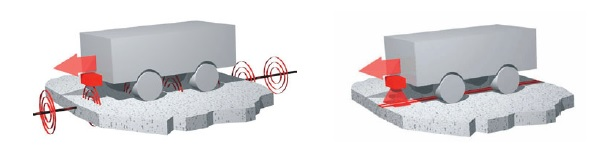
\includegraphics[width=0.9\textwidth]{Prinzipskizze_induktiven.jpg}
	\caption{Prinzipskizze zur induktiven und optischen Spurf\"uhrung (Quelle: G\"unter Ullrich, 2011 S. 79)}
	\label{Prinzipskizze_induktiven}
\end{figure}  
	\item \textbf{Orientierung durch Magnetmarken:} Eine weitere M\"oglichkeit der Steuerung ist die Abtastung von Magnetstreifen oder magnetischen Markierungen auf der Straßenoberfl\"ache. Dabei bedarf es zur Berechnung der Leitlinie einerseits der Koppelnavigation, zus\"atzlich der f\"ur die Peilung in regelm\"a\"ssigen Abst\"anden in den Boden eingelassenen Marken. Diese Marken k\"onnen rein passive Dauermagnete oder aber quasi-aktive Transponder sein (G\"unter Ullrich, 2011 S. 80). Das Bild \ref{Prinzipskizze_Koppelnavigation_rechts} ist eine Repr\"asentation der Navigation durch Magnetstreifen.
	\begin{figure}[h!]
		\centering
			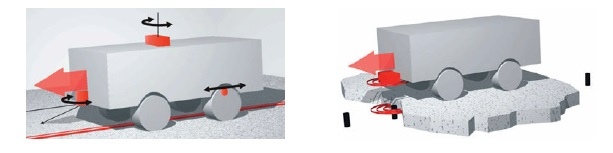
\includegraphics[width=0.9\textwidth]{Prinzipskizze_Koppelnavigation_rechts.jpg}
			\caption{Prinzipskizze zur Koppelnavigation (links) und zur Magnet- bzw. Transpondernavigation (rechts) (Quelle: G\"unter Ullrich, 2011 S. 79)}
			\label{Prinzipskizze_Koppelnavigation_rechts}
	\end{figure}	
	\item Bei der Lasernavigation bestimmt der Laserscanner die Position des FTF, dazu kommen noch optische Sensoren f\"ur Hinderniserkennung z.B. Mensch. Lasergef\"uhrte FTS bieten einen hohen Wert an Flexibilit\"at, da sie ohne Bodeninstallation funktionieren. Nur bei engerem Raum, kann die Lasernavigation nicht so effizient wie z.B. eine induktive Spurf\"uhrung sein, wenn viele Fahrzeuge zum Einsatz kommen. Um die Systemvorteile eine Lasernavigation optimal zu benutzen, ben\"otigt man allerdings ein passendes Anlagenkonzept. Die wichtigen Kriterien sind: die Einbindung in den gesamtbetrieblichen Materialflusssystem, die Anpassung an die vorhandenen Steuerungshierarchien und die optimale Auslegung der Technik in Bezug auf Fahrzeugbauart, Lastaufnahmemittel, Energiekonzept, Kommunikation und Leitsystem. Ein Aspekt, der f\"ur das Laser-gef\"uhrte FTS spricht, ist die Wirtschaftlichkeit. Und dies trotz der Alternativen Elektro-, Low-Cost- sowie induktiv gef\"uhrtes FTS. Letztere lassen sich so einrichten, dass sie auch auf leitdrahtlosen, rein rechnergef\"uhrten Teilstrecken verkehren k\"onnen. Keinerlei kostenintensive Bodeninstallation ben\"otigt dagegen das \"uber Lasersensor gesteuerte, v\"ollig frei navigierende Laser-FTS. Die Fahrzeuge orientieren sich lediglich an im Raum verteilten Reflektoren und mit Hilfe der Kombination von Winkel- und Distanzmessung. (Werner Swoboda, Industrie Anzeiger). Das Bild \ref{Prinzipskizze_Koppelnavigation_links} ist eine Visualisierung der Lasernavigation.
	\begin{figure}[h!]
		\centering
		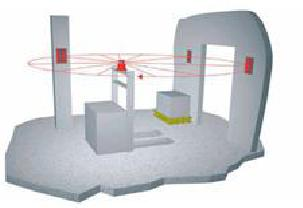
\includegraphics[width=0.8\textwidth]{Prinzipskizze_Koppelnavigation_links.jpg}
		\caption{Prinzipskizze zur Koppelnavigation (links) und zur Magnet- bzw. Transpondernavigation (rechts) (Quelle: G\"unter Ullrich, 2011 S. 79)}
		\label{Prinzipskizze_Koppelnavigation_links}
	\end{figure}

	\item \textbf{Orientierung durch GPS:} Seine Anwendung im Bereich der Fahrzeugsteuerung wird in Form des DGPS eingesetzt, die als Referenzsignal dient. DGPS bedeutet differential GPS und meint die Verwendung eines zus\"atzlichen GPS-Empf\"angers, der nicht auf dem FTF, sondern station\"ar fest installiert ist. Mit Hilfe dieses ortsfesten GPS-Empf\"angers wird der sich zeitlich \"andernde Fehler ermittelt, der dem GPS-System eigen ist. Mit Hilfe dieser Kenntnis k\"onnen zeitgleich die fahrenden GPS-Empf\"anger auf den FTF exakte Positionen ermitteln (Quelle: G\"unter Ullrich, 2011 S. 27). Diese Navigationstechnik braucht eine freie Sichtkegel von 15 Grad  nach oben (siehe Bild 4), m zuverl\"assig arbeiten zu k\"onnen. DieSchritte zur Erlangung der erforderlichen Fahr- und Positioniergenauigkeit sind:
	\begin{itemize}
		\item Pr\"ufung der \"ortlichen Gegebenheiten, insb. der Empfangsst\"arken der Satelliten
 \item Einsatz des Differential-GPS
 \item Real Time Kinematic Differential GPS. 
\end{itemize}
	\begin{figure}[h!]
		\centering
		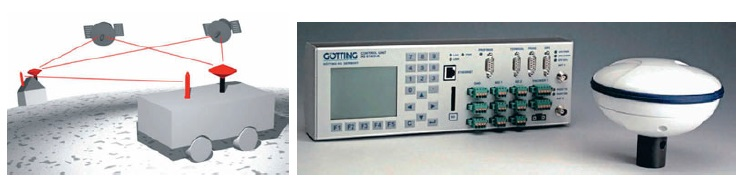
\includegraphics[width=0.9\textwidth]{Prinzipskizze_zur_Navigation_mittels_GPS.jpg}
		\caption{Prinzipskizze zur Koppelnavigation (links) und zur Magnet- bzw. Transpondernavigation (rechts) (Quelle: G\"unter Ullrich, 2011 S. 79)}
		\label{Systemarchitektur_FTS}
\end{figure}
Im Rahmen des Projekt FAISE wird die Navigation durch den Laser durchgef\"uhrt. Es kann hier kein Global Positioning System (GPS) verwendet werden, da das ganze Experiment in einem geschlossenen Raum gemacht wird. Weiterhin es kann auch keine Navigation durch die physische Leitlinie oder durch die St\"utzpunkte im Boden erzielt, weil der Boden gebrochen werden m\"usste.
\end{itemize}

\subsubsection{Steuerungstechnik}
Die interne Materialflusssteuerung ist eine Vorstufe der Transportauftragsabwicklung und wird nur dann ben\"otigt, wenn die Transportauftr\"age nicht klar dezidiert \"ubertragen, sondern aufbereitet werden m\"ussen. Eine Anforderung wie z. B. ben\"otige Ware A an Maschine B erfordert eine Umsetzung in einen oder mehrere Transportauftr\"age nach dem klassischen Muster. Hole von C und Bringe nach D. Die FTS-interne Materialflusssteuerung kombiniert also Quelle und Senke \"uber die in ihr hinterlegten Transportbeziehungen zu einem Transportauftrag und schickt diesen zur Durchf\"uhrung an die Transportauftragsverwaltung. Diese ganze Transportauftragsverwaltung ist in der FTS-Leisteuerung geregelt. 
Die FTS-Leitsteuerung ist die Kommandozentrale, um das FTS in das Umfeld zu integrieren. Au\"sserdem steuert es die FTF, die sich im System befinden. Damit ist das FTS dann in der 
Lage, die ihm \"ubertragenen Auftr\"age zu erf\"ullen. "`Eine FTS-Leitsteuerung besteht aus Hard- und Software. Kern ist ein Computerprogramm, das auf einem oder mehreren Rechnern abl\"auft. Sie dient der Koordination mehrerer Fahrerloser Transportfahrzeuge und/oder \"ubernimmt die Integration des FTS in die innerbetrieblichen Abl\"aufe."' (VDI 4451). Die Leitsteuerung bringt das FTS in seinem Umfeld zusammen, bietet seinen Bedienern vielf\"altige Service-M\"oglichkeiten und nimmt Transportauftr\"age entgegen. Weiterhin stellt sie den Aufgaben entsprechende Funktionsbl\"ocke zur Verf\"ugung. 
Die FTS-Leitsteuerung ist der Kern der FTS. In Rahmen des Projekt FAISE, wird es auch eine Leisteuerung ben\"otigt. Eine Leitsteuerung ist nur mit Hilfe eine Systemarchitektur zu implementieren und zu verstehen. In seinem Buch Fahrerlose Transportsysteme, hat G\"unter Ulrich zwei verschiedene Systemarchitekturen dargestellt. Eine f\"ur eine einfache FTS und eine andere f\"ur eine komplexe FTS. Da es bei FAISE nur mit vier FTF gearbeitet wird, ist es sinnvoll mit einer einfachen Systemarchitektur zu arbeiten. Das Bild 3 ist eine Repr\"asentation einer einfachen Systemarchitektur.
	\begin{figure}[h!]
		\centering
		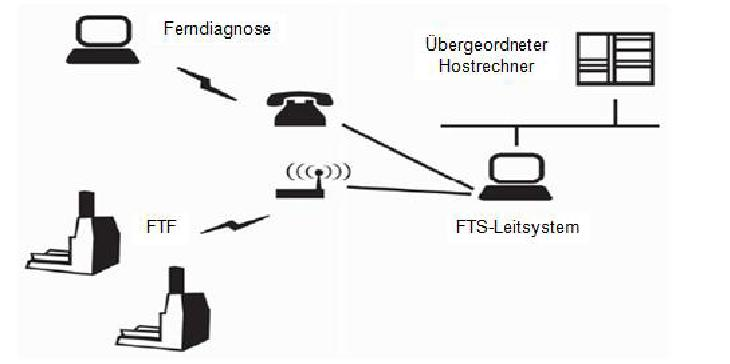
\includegraphics[width=0.9\textwidth]{Systemarchitektur_FTS.jpg}
		\caption{Die Systemarchitektur eines einfachen FTS (Quelle: G\"unter Ullrich, 2011 S. 93)}
		\label{Systemarchitektur_FTS}
	\end{figure}

Es gibt eine geringe Anzahl von FTF, mit denen die Leitsteuerung per WLAN in Verbindung ist. Au\"sserdem gibt es ein LAN, \"uber das es eine direkte Verbindung mit einem \"ubergeordneten Rechner gibt, von dem die Transportauftr\"age kommen. \"uber die angedeutete Telefonleitung ist eine VPN-Verbindung zur Ferndiagnose eingerichtet. Die Daten\"ubertragung zu den \"ubergeordneten Host-Rechnern erfolgt meist \"uber lokale, Ethernet basierte Netzwerke mit dem Protokoll TCP/IP. Solche Host-Rechner k\"onnen beispielweise Materialflusssteuerungssysteme zur Produktionssteuerung (z. B. SAP) Produktionsplanungssysteme (PPS) Lagerverwaltungssysteme (LVS) sein.“( vgl. G\"unter Ullrich, 2011 S. 96). 
Au\"sserdem nach der VDI 4451(Blatt 3) „zum internen Umfeld der FTF-Steuerung geh\"oren das Lastaufnahmemittel (LAM), Sensoren und Aktoren, Bedienfeld am Fahrzeug und das Sicherheitssystem. Das externe Umfeld besteht aus der FTS-Leisteuerung, anderen FTF, automatischen Stationen und Geb\"audeeinrichtungen“. Die Abbildung 1 stellt eine Darstellung eine FTF-Steuerung und ihr Steuerungsumfeld dar.
	\begin{figure}[h!]
		\centering
		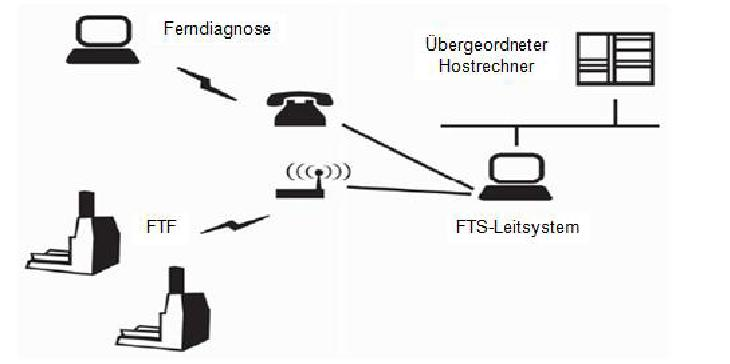
\includegraphics[width=0.9\textwidth]{Systemarchitektur_FTS.jpg}
		\caption{Allgemeine Darstellung einer FTF-Steuerung mit Datenschnittstellen (vgl. VDI 4451)}
		\label{Wertschoepfungskette}
	\end{figure}
Die administrative Ebene, die h\"aufig \"uber einen station\"aren Leitrechner realisiert wird, verwaltet die Transportauftr\"age der ganzen Materialflusssteuerung. Die operative Ebene, die auch als Fahrzeugsteuerung bezeichnet wird, erh\"alt ihre Informationen \"uber die Fahrzeugdisposition der administrativen Ebene. Der Funktionsblock Kommunikation leitet den stattgefundenen Datenaustausch zum Manager weiter. Dieser sorgt f\"ur die Koordination, indem er die Fahrauftr\"age in einzelne Befehle aufteilt, sowie f\"ur ein reibungsloses Zusammenwirken der einzelnen Funktionsbl\"ocke. Neben dem Block Kommunikation sind weitere Bl\"ocke vorhanden. Dazu geh\"ort f\"ur die gesamte Last\"ubergabe inklusive der Lastlagererfassung verantwortliche Lastaufnahme, das Energiemanagement, welches den Lade- und Allgemeinzustand der Batterien \"uberwacht, und der Block \"uberwachung/Sicherheitsschnittstelle, welcher zum Schutz der Personen und Sachgegenst\"ande dient. Der Funktionsblock Fahren und die damit verbundene Sensorik bzw. Aktorik koordinieren die Ablaufsteuerung der Funktionen des Orientierungssystems (Langenbach Maik, 2012, S. 33).

\subsection{Materialflusssysteme}
Damit ein Produkt auf den Markt kommen kann, muss man ihn denken, ihn erstellen und dann ihn vermarken. Die Produkterstellung und -vermarktung sind Prozesse des Wirtschaftens. Vorprodukte oder Materialen werden von Beschaffungsm\"arkten in die Unternehmen gef\"uhrt und dort werden sie durch besondere Produktionsprozesse transformiert. Am Ende der Produktion, steht ein Endprodukt, der f\"ur den Konsum bereits ist. 
Die Produktion und Logistik von G\"utern sind daher sehr wichtige Bereiche f\"ur den Unternehmenserfolg. Allerdings f\"uhren heute die unterschiedlichen Auspr\"agungen der Logistik z.B. in Produktions-, Handels-, oder Verkehrsunternehmen zu einer terminologischen Differenzierung der Logistik. Der Materialflussbegriff leitet sich einfach von dem logistische Konzept ab, in anderen W\"ortern das Materialflusssystem f\"uhrt in der Logistik zur\"uck. Die Abbildung 2. dient zur Erl\"auterung einer konventionellen Wertsch\"opfungskette. 
	\begin{figure}[h!]
		\centering
		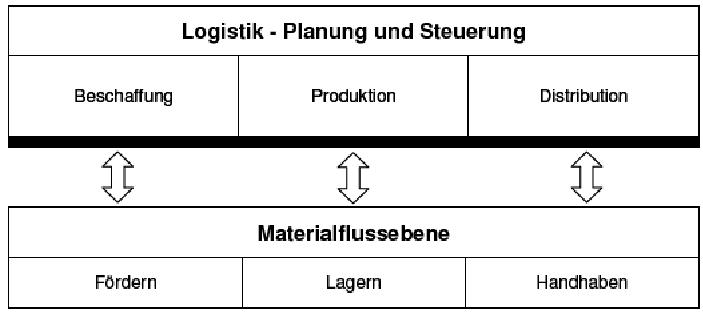
\includegraphics[width=0.9\textwidth]{Wertschoepfungskette.jpg}
	\caption{Elemente einer Wertsch\"opfungskette (vgl. Wulz, J, 2008, S. 7)}
	\label{Wertschoepfungskette}
\end{figure}

Der Begriff Materialfluss bedeutet die Verkettung aller Prozesse bei der Beschaffung, Bearbeitung, Verarbeitung sowie bei der Distribution von G\"utern innerhalb festgelegter Bereiche. Deswegen l\"asst sich der Materialfluss in vier Stufen unterordnet: externer Transport, betriebsinterner Materialfluss, geb\"audeinterner Materialfluss und Materialfluss am Arbeitsplatz. Nach dem Verein Deutscher Ingenieur bzw. VDI-241 beinhaltet die Logistik f\"unf Hauptfunktionen. Diese Funktionen sind Bearbeiten, Pr\"ufen, Handhaben, F\"ordern, Lagern und Aufenthalten. Neben diesen Hauptfunktionen z\"ahlen auch Nebenfunktionen wie z.B. Montieren, Umschlagen, Kommissionieren, Palettieren und Verpacken (VDI 2411). Jedoch ist auf der Ebene des Materialflusssystems nur drei Funktionen zu ber\"ucksichtigen: F\"ordern, Lagern, Handhaben. Die anderen Funktionen setzen sich normalerweise aus den erl\"auterten Funktionen zusammen. Dieses Arbeitsteil wird in zwei Teile gegliedert. Im ersten Teil werden die drei Funktionen der Materialflusssysteme vorgestellt Im zweiten Teil wird eine Planung von Materialflusssystemen dargestellt.

\paragraph{Funktionen von Materialflusssystemen}
\begin{itemize}
	\item \textbf{Funktion F\"ordern} \\
	F\"ordern bedeutet Transportieren und ist eine der wichtigsten Aspekte innerhalb des Materialflusssystems. Nach der VDI 2411 ist F\"ordern das Fortbewegen von Arbeitsgegenst\"anden in einem System. „Die Fortbewegung oder Ortver\"anderung von G\"utern oder Personen mit technischen Mitteln wird allgemein als Transport bezeichnet. Findet diese Ortsver\"anderung in einem r\"aumlich begrenzten Gebiet wie beispielsweise innerhalb eines Betriebes oder Werkes statt, so wird dieser Vorgang durch den Begriff F\"ordern pr\"azisiert. Das F\"ordern bzw. die F\"ordertechnik umfasst also das Bewegen von G\"utern und Personen \"uber relativ kurze Entfernungen einschlie\"sslich der dazu notwendigen technischen organisatorischen und personellen Mittel“(Ten Hompel, Schmidt, Nagel, 2007, S. 119). 
Das F\"ordermittel (technisches Transportmittel, zur Ortsver\"anderung von G\"utern oder Personen) und das F\"orderelement bilden das physikalische Bestandteil eines F\"ordervorgang. Der Ablauf und die Steuerung werden durch den F\"ordervorgang dargestellt. In Punkto F\"ordermittel kann auf verschiedenste Elemente der Materialflusstechnik zur\"uckgegriffen werden. Dies umfasst unter anderen Rollenbahnen, und FTS. Neben der M\"oglichkeit auf automatisierte F\"ordermittel zur\"uckzugreifen, kommen auch manuell mechanisierte bzw. rein manuelle Systeme zum Einsatz. In diesem Fall ist der Mensch oder der Bediener eines F\"ordermittels wesentlich f\"ur den Ablauf eines reibungslosen Materialflusses in Zusammenspiel mit den physikalischen Elementen sowie dem Prozessablauf verantwortlich. (Wulz, J, 2008, S. 8). Das Bild 4 gilt als Beispiel eines F\"ordersystems. 
	\begin{figure}[h!]
	\centering
  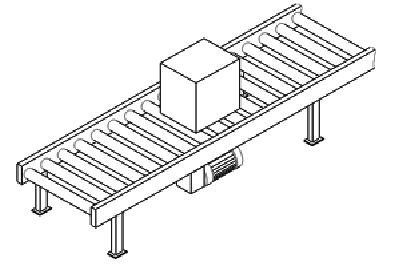
\includegraphics[width=0.7\textwidth]{Stetigfoerderer.jpg}
	\caption{Beispiel eines Stetigf\"orderer (entnommen aus Ten Hompel, Schmidt, Nagel, 2007, S. 131)}
	\label{Stetigfoerderer}
\end{figure}

\item \textbf{Funktion Lagern} \\
Das Lagern ist jedes geplante Liegen des Arbeitsgegenstandes im Materialfluss. Das Lager ist ein r\"aumlich abgegrenzter Bereich bzw. eine Fl\"ache zum Aufbewahren von St\"uck- und/oder Sch\"uttg\"utern in Form von Rohmaterialien, Zwischenprodukte oder Endprodukte, das mengenm\"a\"ssig erfasst wird (VDI-2411). Die Einlagerung von Lagereinheiten, die Aufbewahrung und Bereithaltung von Lagereinheiten auf Lagerpl\"atzen und die Auslagerung einer Lagereinheit, sind die grundlegenden Prozesse in einem Lager.
Aufgrund der starken Ver\"anderungen im Markt, m\"ussen auch die unternehmerischen Abl\"aufe an Lagersysteme schnell angepasst werden. In einem Lagersystem werden im Verlauf des Materialflusses Speicher- bzw. Lagerfunktionen sowie F\"orderfunktionen wahrgenommen. 
Aufgabe eines Lagers ist das Bevorraten, Puffern und Verteilen von G\"utern. W\"ahrend Vorratslager lang- und mittelfristige und Pufferlager kurzfristige Bedarfsschwankungen ausgleichen sollen, erf\"ullen Verteillager neben der Bevorratungs- noch eine Kommissionierfunktion. Daher k\"onnen die Aufgaben eines Lagers anhand folgender Ausgleichsma\"ssnahmen beschrieben werden: Zeitausgleich, Mengenausgleich, Raumausgleich und Sortimentsausgleich. (Stich, V.; Bruckner, A.; 2002). Ein Zeitausgleich ist immer dann erforderlich, wenn die Zeitfunktion der Nachfrage nicht der Zeitfunktion der Produktion entspricht. Beispielsweise steht eine losgr\"o\"ssenoptimierte Fertigung einer saisonalen Nachfrage gegen\"uber. Gerade in Bereichen mit Serienfertigung, in denen aus Kostengr\"unden in der Regel gr\"o\"ssere Mengen als die Nachfragemengen produziert werden, muss Mengenausgleich vollzogen werden. Sobald der Produktionsort nicht mit dem des Produktabnehmers \"ubereinstimmt, findet mit Hilfe von Verkehrstr\"agern ein Raumausgleich statt. Mit zunehmender Sortimentsbreite steigt die Wahrscheinlichkeit, dass die Anzahl der Produktionsstandardorte steigt. (Lagenbach, M, 2012, S. 14).

\item \textbf{Funktion Handhaben } \\
Der Begriff Handhaben wurde gedanklich von de menschlichen Hand abgeleitet, wird aber auch f\"ur automatische ablaufende Vorg\"ange zur Manipulation von Objekten gebraucht. Handhaben bedeutet etwas greifen, bewegen und an einem bestimmten Ort ablegen. Das hei\"sst, durch Handhaben wird die Lage oder Position von Objekten ge\"andert. Im \"ubertragenen Sinne bedeutet handhaben auch bewerkstelligen bzw. praktisch aus\"uben. Von Handhabungstechnik spricht man, wenn f\"ur die Handhabung Ger\"ate eingesetzt werden. 
Die Richtline VDI 2860 definiert die Funktion Handhaben als „das Schaffen, definiertes Ver\"andern oder vor\"ubergehendes Aufrechterhalten einer vorgegebenen r\"aumlichen Anordnung von geometrisch bestimmten K\"orpern.“ Die Teilfunktionen des Handhabens stellen das Speichern, das Bewegen, das Sichern, das Kontrollieren und das Ver\"andern von G\"utern dar. Das Handhaben kann sowohl als eine Funktion als auch eine Fertigung des Materialflusses betrachtet werden. Eine m\"ogliche Handhabungsfunktion im Materialfluss ist z.B. das Palettieren, worunter die Stapelung von St\"uckg\"utern zu einem St\"uckgutstapel nach einem gewissen Muster verstanden wird. Handhabungsfunktionen k\"onnen entweder von Automaten z.B. Roboter oder von Menschen durchgef\"uhrt werden. Auf Grund der Greifflexibilit\"at ist der Mensch jedoch meist un\"ubertroffen in der Handhabung.
\end{itemize}

\subsection{Fallbeispiele}
\subsubsection{FTS in der Gl\"asernen Manufaktur Dresden (Volkswagen)}
Volkswagen AG montiert das neue Modell der Luxusklasse "Phaeton" in der "Gl\"asernen Manufaktur" in Dresden. Die Materialversorgung \"ubernimmt ein fahrerloses Transportsystem mit 56 frei navigierenden Fahrzeugen. Die gesamte Steuerungs- und Navigationstechnik stammt von FROG Navigation Systems, dem Projektpartner des Generalunternehmers AFT (Mechanik).
Die Produktion ist auf drei Ebenen unterteilt: . Die eigentliche Montage findet auf den beiden oberen Montageebenen statt: Die Rohrkarosse befindet sich auf einer Montageplattform, die Teil des Schuppenbandes ist, das sich sicher in den Hallenboden einf\"ugt und mit konstanter Geschwindigkeit durch die Montagezyklen bewegt. Danach erfolgt die \"ubergabe an eine schwere Elektroh\"angebahn (EHB) zur H\"angemontage. W\"ahrend der H\"angemontage erfolgt die Hochzeit, d. h. das Zusammenf\"ugen von Karosse und Triebsatz, wobei der Triebsatz von einem Fahrerlosen Transportfahrzeug (FTF) herangebracht wird. Anschlie\"ssend wird die Karosse wieder auf eine Schubplattform, die sog Schuppe, zur Komplettierung und Qualit\"atskontrolle gestellt.

Im Untergeschoss, der Logistikebene, wird die verbauende Ausr\"ustung zur Verf\"ugung gestellt und in Betrieb genommen. Die FTS \"uberminnt die Versorgungsleitungen der Materialien und damit eine erhebliche logistische Funktion . Um zwischen den Ebenen zu wechseln, nutzen die  automatischen Fahrzeug-Hebeb\"uhnen .
Das FTS hat die grunds\"atzliche Aufgabe, die Montagelinien (Schuppenband oder EHB) zu versorgen. Dabei wird allerdings zwischen folgenden sechs Gewerken unterschieden:
\begin{itemize}
\item[1.] Anlieferung von Warenk\"orben auf die Schuppe
\item[2.] Anlieferung von Schalttafeln (Cockpits)
\item[3.] Anlieferung von Kabelstr\"angen
\item[4.] Anlieferung des Triebwerks mit Fahrwerk und Ausf\"uhrung der Hochzeit
\item[5.] Anlieferung von Warenk\"orben zur H\"angemontage
\item[6.] Anlieferung der T\"uren plus Warenk\"orbe
\end{itemize}
\subsubsection{FTS beim Automobilhersteller BMW im Werk Leipzig}
Das BMW-Werk in Leipzig hat im Jahre 2005 mit der Produktion der 3er reihe (E90) gestartet
Im Bereich der Teileversorgung \"ubernimmt erstmals in der Geschichte der Automobilindustrie ein Fahrerloses Transportsystem (FTS) umfangreiche Logistikfunktionen. Folgende Prozesse wurde f\"ur die Teilversorgung im Leipzig-Werk definiert:

\begin{itemize}
\item Direktanlieferung per LKW: Gro\"sse Teile mit geringer Komplexit\"at (z. B. Bodenmatte oder Kofferraumverkleidung) werden per LKW zeitnah und in unmittelbare N\"ahe des Verbauortes angeliefert.
\item Modulanlieferung per EHB8: Gro\"sse und komplexe Baugruppen (z. B. Cockpit) werden direkt auf dem Werksgel\"ande von externen Lieferanten oder BMW Mitarbeitern montiert.
\item Lagerware per FTS: Die Mehrzahl der Teile wird in einem Versorgungszentrum gelagert, kommissioniert und mit Fahrerlosen Transportfahrzeugen (FTF) an die jeweiligen Verbauorte in der Montage gebracht (G\"unter Ullrich, 2011 S. 36).\end{itemize}
Es sind 74 FTF im Einsatz, als Ladehilfsmittel werden mehr als 2.000 Rollwagen in zwei unterschiedlichen Ausf\"uhrungen eingesetzt. Je FTF werden entweder zwei kleine Rollwagen, zur Aufnahme von Beh\"altern bis DIN-Gr\"o\"sse, oder ein so genannter \"ubergro\"sser Rollwagen zur Aufnahme von Gro\"ssbeh\"altern eingesetzt. Zus\"atzlich gibt es noch die Sequenziergestelle mit Sonderaufbauten (G\"unter Ullrich, 2011 S. 37). Durch einen Laser-Scanner auf dem FTF wird den Personenschutz und Hinderniserkennung \"ubernommen. 

Die Fahrerlosen Transportfahrzeuge finden ihren Weg mit Hilfe der so genannten freien Navigation. Damit ist gemeint, das die Fahrzeuge ohne physikalische Leitspuren und nach einem kombinierten Prinzip aus Kopplung und Peilung arbeiten. Kopplung bedeutet die Auswertung von fahrzeuginternen Sensoren (Messr\"ader und ein faseroptischer Kreisel), wodurch der zur\"uckgelegte Weg samt Kurven bestimmt wird (G\"unter Ullrich, 2011 S. 37). Bei jeder Peilung werden aufgetretene Fahrfehler, die durch Schlupf der R\"ader oder durch Ver\"anderungen des Raddurchmessers auftreten k\"onnen, korrigiert. Die Vorteile dieses, auch Magnet Navigation genannten, Verfahrens liegen in der Zuverl\"assigkeit und der Flexibilit\"at bei zuk\"unftigen Layoutanpassungen (G\"unter Ullrich, 2011 S. 37).



	
	% Chapter 3 Projektorganisation
	\clearpage
	\ohead[Projektorganisation]{Projektorganisation}
	\chead[Uni Oldenburg]{Uni Oldenburg}
	\ihead[PG FAISE]{PG FAISE}
	\setheadtopline{1pt}
	\setheadsepline{0.5pt}
	\ofoot[Endbericht]{Endbericht}
	\cfoot[\pagemark]{\pagemark}
	\ifoot[30. September 2014]{30. September 2014}
	\setfootsepline{0.5pt}
	\setfootbotline{1pt}
	\section{Projektorganisation}
Die nachfolgenden Abschnitte beschreiben den organisatorischen Ablauf innerhalb der Projektgruppe. Dazu geh\"ort die Aufteilung in Gruppen, sowie die zeitliche Planung und Rollenverteilung. Des weiteren werden hier das Vorgehen f\"ur das gesamte Projekt und die verwendeten Werkzeuge beschrieben.

\subsection{Organisation der Teilgruppen (Materialfluss, Fahrzeuge, Simulation)}
Die Projektgruppe ist in die drei Teilgruppen unterteilt,  da das Gesamtprojekt in eindeutig abgrenzbare Aufgabenfelder gegliedert ist und so Kompetenzen und Verantwortlichkeiten klar definiert werden können. 

\begin{itemize}
\item \textbf{Materialfluss} \\
Die Teilgruppe Materialfluss befasst sich mit Programmierung der Sensorik und Aktorik für die Rampen, sowie dem Aufbau eines Sensornetzwerkes zur Kommunikation zwischen den verschiedenen Akteuren der Simulation. 

\item \textbf{Fahrzeuge} \\
Die Teilgruppe Fahrzeuge befasst sich mit allen Aspekten, die für das Funktionieren der Fahrzeuge verantwortlich sind. Dazu zählen unter anderem die Navigation, Odometrie und Lokalisierung. Auch ist die Einrichtung der Versorgungsinfrastruktur für die Fahrzeuge in Form von Ladestationen f\"allt in den Aufgabenbereich der Fahrzeuggruppe. Zusammen entwickeln die Teilgruppen Fahrzeuge und Materialfluss das physische System, so dass Kommunikation und Abstimmung zwischen diesen beiden Gruppen besonders wichtig sind. 

\item \textbf{Simualtion} \\
Die Teilgruppe Simulation entwickelt die Software mit der eine virtuelle Simulation erstellt wird. Diese Software beinhaltet einen hybriden Modus, in dem das physische System auf die Software abgebildet wird und beide Teilsysteme ein Gesamtsystem bilden. Für die Entwicklung des Hybridmodus muss ein funktionierendes physisches System vorliegen.
\end{itemize}

\subsection{Rollenverteilung}

Um organisatorische Aspekte innerhalb des Projektes besser umsetzen zu k\"onnen, wurden unterschiedliche Rollen definiert, die jeweils einen Bereich des Projektes abdecken sollen. Dazu geh\"oren folgende Aufgaben:

\begin{itemize}
\item\textbf{Administrator}

Der Administrator ist f\"ur die Einrichtung und Betreuung der Server und Tools zust\"andig, dazu z\"ahlt auch die Einrichtung der Webseite.

\item \textbf{Aussendarstellung}

Um das Projekt vern\"unftig zu Repr\"asentieren, verwalten die zust\"andigen der Aussendarstellung den Inhalt der Webseite. Ausserdem sind sie f\"ur die externen Kontakte und Events / Pr\"asentationen verantwortlich.

\item \textbf{Dokumentenbeauftragte}

Damit am Ende ein einheitliches Format f\"ur den Endbericht gilt, organisieren, sammeln und verwalten die Beauftragten jegliche Quellen und Berichte ( dazu z\"ahlt auch das Repository ). Des weiteren sind sie Ansprechpartner bei fragen zur Literatur.

\item \textbf{Gruppenleiter}

Da das Projekt aus drei Teilgruppen besteht, besitzt jede Gruppe einen eigenen Gruppenleiter, der die Prozesse innerhalb der Gruppe lenkt und gemeinsam mit den anderen Gruppenleitern das gesamte Projekt koordiniert.

\item \textbf{Qualit\"atsmanagement}

Damit der Projektplan eingehalten wird, ist es Aufgabe des Qualit\"atsmanagements, dass die Prozesse ( Scrums ) eingehalten und korrekt ausgef\"urt werden. Zus\"atzlich sind sie f\"ur die System und Integrationstests verantwortlich.

\item \textbf{Werkzeugbeauftragte}

Die Werkzeugbeauftragen verwalten die ben\"otigten Ger\"ate und Schl\"ussel f\"ur die gesamte Projektgruppe. Weiterhin regeln sie, mit R\"ucksprache mit den Betreuern, den Einkauf der Hardware und Software.

\end{itemize}


\subsection{Vorgehensmodell}
Für die Durchführung der Projektgruppe muss ein Vorgehensmodell, sowohl für die Gesamt- als auch für die Teilgruppen, festgelegt werden. Durch ein Vorgehensmodell wird die Arbeit im Team strukturiert und es wird festgelegt, wie bestimmte Aufgaben, wie z.B. Abgleich mit Kunden und Anwendern, umgesetzt werden sollen. Sowohl für die Teilgruppen als auch für die Gesamtgruppe wurde ein Scrummodell als Vorgehensmodell gewählt ( siehe Abbildung 9).

	\begin{figure}[h!]
		\centering
			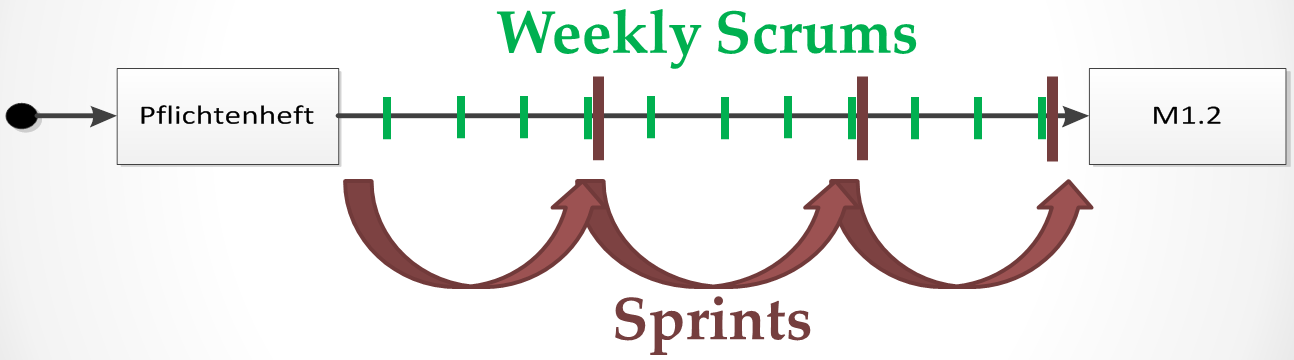
\includegraphics[width=0.9\textwidth]{Projektorganisation_Scrum.png}
			\caption{Scrumplanung f\"ur einen Meilenstein}
			\label{Projektorganisation_Scrum}
	\end{figure}	

Da es für ein sehr komplexes Projekt, wie das vorliegende, schwierig ist nur von einer groben Vision, sowie von User Stories auszugehen, wurden zun\"achst auf Basis des vorliegenden Lastenhefts in jeder Teilgruppe Pflichtenhefte erstellt. Anschließend wurden die dazugeh\"origen User Stories definiert, die die Anforderungen aus dem Pflichtenheft ber\"ucksichtigen und aus Anwendersicht darstellen. Die Sprints in den Teilgruppen sind mit einem Monat bemessen und werden zur Durchf\"uhrung der User Stories genutzt. Die Rolle des Product Owners wird von den beiden Betreuern eingenommen, die sowohl für die Teil- als auch für die Gesamtgruppen zur Verfügung stehen, um die entwickelten Funktionalit\"aten abzugleichen.
Die Durchf\"uhrung von Daily Scrums ist zeitlich nicht m\"oglich, da es sich um eine studentische Projektgruppe handelt, deren Stundenplan keine t\"aglichen Treffen erm\"oglicht. Deshalb wurde das Scrum Vorgehensmodell dahingehend angepasst, dass die Daily Scrums in Weekly Scrums abgewandelt wurden. Die Weekly Scrums finden sowohl in den Teilgruppen als auch in der Gesamtgruppe statt. In den Weekly Scrums der Gesamtgruppe wird zun\"achst von jeder Person berichtet, welche Aufgaben in der vorherigen Woche erledigt wurden, damit entstandene Probleme und Hindernisse direkt in der Gruppe besprochen und eventuell beseitigt werden k\"onnen. Die Ergebnisse aus den Teilgruppen werden ebenfalls vorgestellt und mit den Product Ownern abgeglichen.
Das Scrum Vorgehensmodell wird mit  Prototyping kombiniert ( siehe Abbildung 10 ).

Durch das Prototyping sollen zu bestimmten Meilensteinen die kombinierten Ergebnisse aus den Teilgruppen vorgestellt werden, um den Stand des Gesamtsystems begutachten zu k\"onnen. Betrachtet man das gesamte Projekt, so besteht es aus 2 Prototyping Phasen. Diese trennen sich im zweiten Meilenstein. Bis zu diesem Zeitpunkt wird mit horizontalen Prototyping die Basis des Projektes geschaffen. Das bedeutet, dass alle Grundfunktionalit\"aten implementiert und umgesetzt werden. Danach folgt das vertikale Prototyping in dem die Funktionalit\"aten um weitere Aspekte und Feinheiten er\"anzt werden. Innerhalb dieser beiden Phasen kommt es immer wieder zu Aufgabenbereichen, die jede Teilgruppe f\"ur sich umsetzt. Ebenfalls sind Phasen vorhanden, in denen die Ergebnisse der einzelnen Gruppen zusammengef\"uhrt werden m\"ussen, wodurch das Zusammenspiel zwischen dem Materialfluss und der Volksbots, sowie die Darstellung in der Simulation, entsteht.

	\begin{figure}[h!]
		\centering
			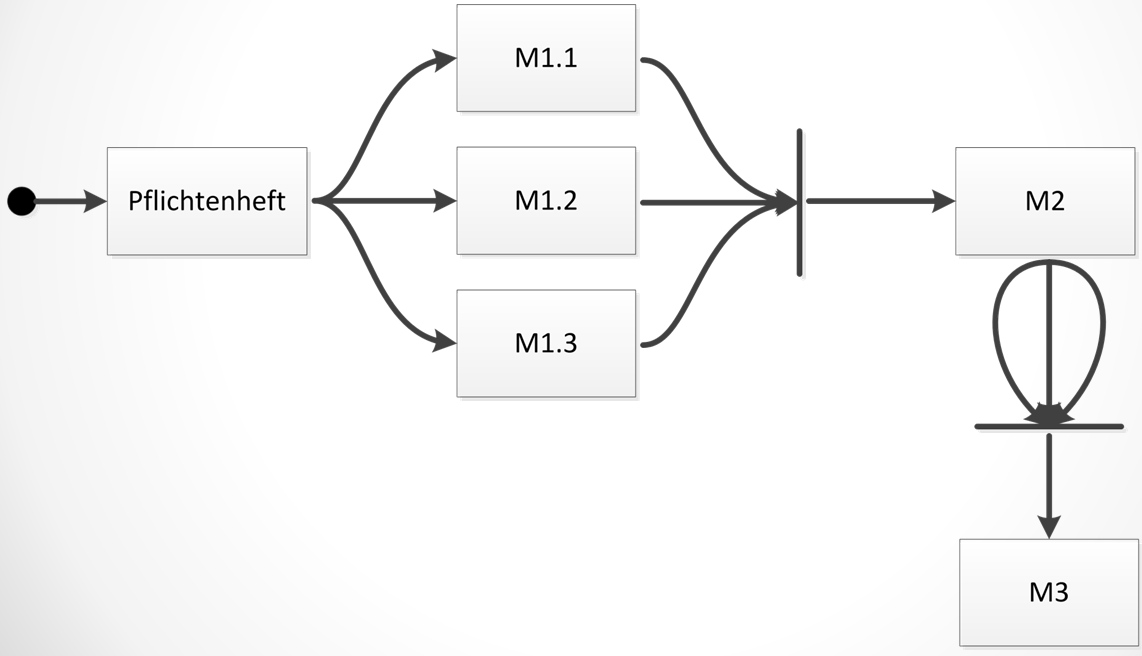
\includegraphics[width=0.9\textwidth]{Vorgehensmodell_Prototyping.png}
			\caption{Modell für die Darstellung der einzelnen Projektphasen}
			\label{Vorgehensmodell_Prototyping}
	\end{figure}	

\subsection{Werkzeuge}	

Zur Unterstützung der Zusammenarbeit in der Projektgruppe wurden verschiedene Werkzeuge ausgewählt um die Kollaboration zu vereinfachen. Um eine gute Verknüpfung der Werkzeuge zu gewährleisten, wurde versucht die Produkte aus einer Hand zu beziehen. Nach einiger Recherche, stachen zwei Möglichkeiten heraus. Entweder die Open-Source Software Redmine oder eine kommerzielle Lösungen von der Firma Atlassian.

Die beiden Lösungen wurden daraufhin auf Basis verschiedener Kriterien verglichen. Zu diesen Kriterien zählten mitunter Usability, Verbreitung am Markt, Stabilität und Wartbarkeit.

Die Evaluation ergab Atlassian als klaren Sieger und die Projektgruppe einigte sich im speziellen auf die Werkzeuge \textbf{Jira} und \textbf{Confluence}. 

\begin{figure}[h!]
		\centering
			
\includegraphics[width=0.5\textwidth]{logoAtlassian.png}
			\caption{Hersteller der Projektwerkzeuge}
			\label{Vorgehensmodell_Prototyping}
	\end{figure}

\subsubsection{Jira}
Jira ist ein Projektmanagement-Tool. Neben dem Verwalten von Vorgängen und Fehlern, lässt sich Jira mit einer \textit{Agile} Erweiterung sehr gut zum planen, steuern und verwalten von Sprints. Eine einfache Übersicht über die verschiedenen, anstehenden Aufgaben können die Projektmitglieder über die sogenannten Boards erhalten. Hier wird genau für die verschiedenen User Stories deren Fortschritt angezeigt und welches Projektmitglied gerade welche Aufgabe bearbeitet.

\subsubsection{Confluence}
Confluence ist ein Wiki welches sich sehr gut in Jira integriert. So muss die Benutzerverwaltung nur einfach in Jira eingerichtet werden. Confluence greift dann auf das Benutzerverzeichnis von Jira zurück. 

	
	% Chapter 4 Allgemeine Anforderungen
	\clearpage
	\ohead[Allgemeine Anforderungen]{Allgemeine Anforderungen}
	\chead[Uni Oldenburg]{Uni Oldenburg}
	\ihead[PG FAISE]{PG FAISE}
	\setheadtopline{1pt}
	\setheadsepline{0.5pt}
	\ofoot[Endbericht]{Endbericht}
	\cfoot[\pagemark]{\pagemark}
	\ifoot[30. September 2014]{30. September 2014}
	\setfootsepline{0.5pt}
	\setfootbotline{1pt}
	\section{Komponentenbeschreibung}
\subsection{Mikrocontroller}
Ein Mikrocontroller ist ein kleiner Computer auf einem einzelnen Halbleiter-Chip. Dazu geh\"ort ein Prozessor, der Programme ausf\"uhren kann, Arbeits- und Programmspeicher sowie Schnittstellen, die eine Kommunikation mit der Umgebung erm\"oglichen sog. Peripheriefunktionen \cite{Wikibooks:2014:Online}. Mit ihnen lassen sich komplexe Aufgaben l\"osen, f\"ur die sonst ein aufw\"andiger Schaltungsaufbau notwendig w\"are. Standardm\"a{\ss}ig sind folgende Bestandteile in Mikrocontrollern integriert:
CPU, SRAM und Flash-Speicher f\"ur den Programmcode. Weiterhin bieten MCs analoge und digitale Ports, mehrere AD/DA-Wandler, Timer und Schnittstellen zur Kommunikation mit der Au\"{ss}enwelt \cite{Viktor:Seib:2014:Online}. In der nachstehenden Abbildung ist der allgemeine schematische Aufbau eines Mikrocontrollers in folgender Abbildung dargestellt.
\begin{figure}[h!]
	\centering
		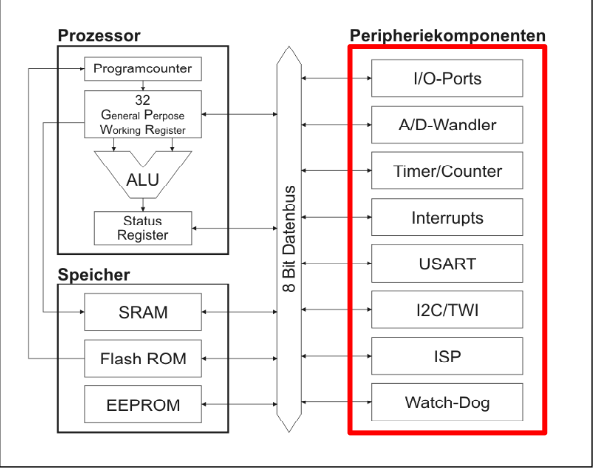
\includegraphics[width=0.9\textwidth]{Aubau_eines_Mikrocontrollers.png}
	\caption{schematischer Aufbau eines Mikrocontrollers \cite{habil:Ostermeye:2014:Online}}}
	\label{Aufbau eines Mikrocontrollers}
\end{figure}

\begin{itemize}
\item Prozessor (CPU)
\begin{itemize}
          \item Arithmetic Logic Unit kurz ALU (Rechenwerk)
          \item 32 GPIO-Register (Arbeitsregister f\"ur ALU)
          \item Programmcounter (Programmposition)
					\item Statusregister (Status der aktuellen Operation) 
\end{itemize}
\item Speicher
\begin{itemize}
          \item SRAM– Datenspeicher (Static Random-Access Memory)
					\item Flash ROM– Programmspeicher (Read Only Memory)
					\item EEPR OM– Festspeicher (Electrically Erasable Programmable Read-Only Memory)
\end{itemize}
\item Peripheriekomponenten
    \begin{itemize}
          \item I/O-Ports Prim\"arfunktion der Pins (Ein- und Ausg\"ange)
          \item A/D-Wandler (Einlesen von analogen Spannungen)
          \item Timer/Counter (Zeitintervall-/PBM-Generator)
					\item Interrupts (Programmunterbrechungsroutinen)
					\item USART, I2C/TWI und SPI (Kommunikationsschnittstellen)
					\item Watch-Dog (Absicherung gegen Systemfehler)
					\item ISP (Schnittstelle zum \"{u}bertragen des kompilierten Programms)
	\end{itemize}
\end{itemize}
Mikrocontroller sind im heutigen Leben weit verbreitet und es gibt eine viele Anzahl von Herstellern, die mikrocontroller anbieten. Im folgenden werden einige Hersteller mit ihren MC-Familien beispielhaft aufgef\"urt:
\begin{itemize}
\item Intel (8051-Serie)
\item Renesas (H8)
\item Zilog (Z8)
\item Microchip (Pic)
\item Freescale (fr¨uher Motorola) (68HC08 bzw. 68HCS08)
\item Atmel (AVR, 8051-Serie)
\end{itemize}
F\"ur das Projekt FAISE wurde das Atmel-Serie eingesetzt. Es sind Mikrocontroller mit erweiterten Peripherien und Funktionen, die auf der 8-Bit-AVR-Architektur basieren. Bei AVR handelt es sich um einen RISC-Kern, der an der Universit\"at von Trondheim in Norwegen entwickelt und von Atmel aufgekauft wurde. Die CPU besitzt 32 allgemeine 8-Bit Register (general purpose registers) und ist in der Lage in einem einzigen Taktzyklus Daten aus zwei beliebigen Registern in die ALU zu laden, diese zu verarbeiten und das Ergebnis in einem beliebigen Register zu speichern \cite{Viktor:Seib:2014:Online}. Die Konfiguration eines Atmega 8 der Firma Atmel sieht so aus:
\begin{figure}[h!]
	\centering
		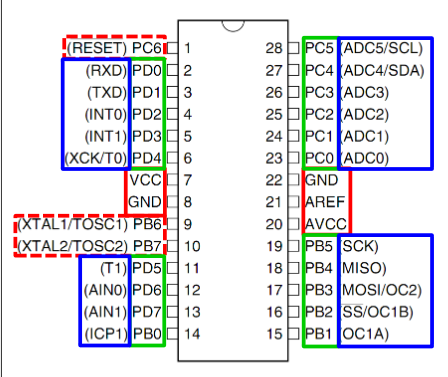
\includegraphics[width=0.9\textwidth]{Atmel8.png}
	\caption{Atmel 8 \\ \url{(http://www.ids.tu-bs.de/tl\_files/Lehre/Vorlesungen/Simulation2/Einfuehrung\_in\_die\_MC\_Programmierung\_Teil1.pdf)}}
	\label{Atmel 8}
\end{figure}
\begin{figure}[h!]
	\centering
		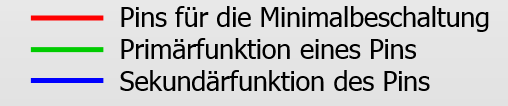
\includegraphics[width=0.9\textwidth]{LegendeAtmel8.png}
	\caption{Atmel 8 \URL{(http://www.ids.tu-bs.de/tl\_files/Lehre/Vorlesungen/Simulation2/Einfuehrung\_in\_die\_MC\_Programmierung\_Teil1.pdf)}}
	\label{Legende Atmel8}
\end{figure}
\begin{itemize}
\item Pins f\"ur die Minimalbeschaltung
\begin{itemize}
          \item Spannungsversorgung
          \item ReferenzspannungTaktgeber
          \item Reset      
					\end{itemize}
\item Prim\"arfunktion eines Pins
\begin{itemize}
          \item Ein- bzw. Ausgang
					\end{itemize}
\item Sekund\"arfunktion des Pins
\begin{itemize}
          \item A/D-Wandlereingang
          \item Ext. Interrupt
          \item PBM-Ausgang   
\end{itemize}
\end{itemize}
F\"ur die Programmierung der AVR-Controller gibt es eine kostenlose Entwicklungsumgebung AVR-Studio, die das Einbinden des Compilers problemlos erlaubt.

\subsection{Sensorik/ Aktorik}
Hauptziel der Teilgruppe Materialfluss ist das Management von Paketen auf einer Rampe. Die Aufgabe der Sensorik ist dabei, die mit Lichtschranken ausgestatteten Rampen Paketen zu detektieren und auf \"Anderung der Position der Paketen zu reagieren. Die Lichtschranken bestehen aus einer Lichtstrahlenquelle (dem Sender) und einem Sensor (dem Empf\"anger) f\"{u}r diese Strahlung. Als Lichtquelle kommt Infrarotlicht zum Einsatz und der Vorteil besteht in der einfachen Einstellung des Sensorsystems durch den sichtbaren Lichtfleck. Das Funktionsprinzip der Lichtschranke besteht darin, der zu  \"andernden Zustand durch die Lichtintensit\"at mit dem Sensor zu registrieren. 
Die Rampen werden auf Hardwareebene um eine Aktorik zum Arretieren der Kisten erg\"anzt. Diese Aktoren (in unserem Fall die eingesetzte Bolzenpaar) sind f\"ur das Ausf\"uhren von Bewegungen zust\"andig. Sie sind aktive Stellelemente, die in der Antriebs - und Steuerungstechnik, die vom  Mikrorechner angesteuert werden und das Verhalten des Prozesses durch das vom Sensor kommende Signal in einer gew\"{u}nschten Weise zu erm\"oglichen. In dieser allgemeinen Darstellung stehen die Ausgangssignale eines Sensors und die Stellsignale der Aktoren mit einem
Informationsverarbeitungssystem (IVS) in Verbindung.

\subsection{Contiki}
Contiki ist ein Open Source Echtzeitbetriebssystem, das bei uns in der PG auf den MICAz-Modulen eingesetzt wird.
Contiki bietet einen einfachen ereignisgesteuerten Betriebssystemkern mit sogenannten Protothreads, optionalem pr\"aemptiven Multiprogramming, Interprozesskommunikation via Messagepassing durch Events, eine dynamische Prozessstruktur mit Unterst\"utzung f\"ur das Laden und Entladen von Programmen, nativen TCP/IP-Support \"ber den uIP TCP/IP-Stack und eine grafische Benutzerschnittstelle, welche direkt auf einem Bildschirm oder als virtuelle Anzeige \"uber Telnet oder VNC genutzt werden kann \cite{Wikipedia:2013:Online}.
 
\subsubsection{Systemarchitektur}
Ein laufendes Contiki System besteht aus dem Kernel, Bibliotheken, Prozessen und dem Programm-Lader, mit dem Anwendun-
gen zur Laufzeit aus dem Speicher oder \"uber ein Funkmodul geladen werden k\"onnen. Die unter stehende Abbildung zeigt die Aufteilung des Betriebssystems in zwei Teile. 
\begin{figure}[h!]
	\centering
		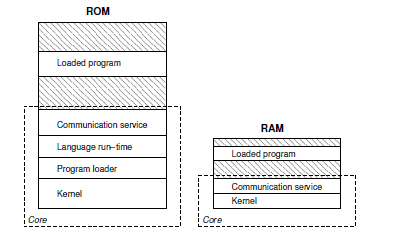
\includegraphics[width=0.9\textwidth]{Systemarchitektur_Contiki.png}
	\caption{Adam Dunkels, Bj\"orn Gr\"onvall, Thiemo Voigt: Contiki - a Lightweight and Flexible Operating System for Tiny Networked Sensors. \url{(Quelle:http://www.up.edu.ps/ocw/upinar/moodledata/872/moddata/assignment/970/1287/10.1.1.59.2303.pdf)}}
	\label{Systemarchitektur von Contiki}
\end{figure}
Der Core ist ein Basissystem und besteht aus dem Kernel, Bibliotheken, Ger\"{a}tetreiber und der Programm-Lader. Im allgemeinen sind \"Anderungen am Core nicht vorgesehen und nur unter Verwendung eines speziellen Bootloader m\"oglich. Die konkrete Aufteilung des Systems in Core und ladbare Programme wird beim Kompilieren des Systems entschieden und h\"angt von der Hardware-Plattform ab \cite[S. 7]{Walter:2010}. Ger\"atetreiber werden als Bibliotheken implementiert. 

\subsubsection{Events}
In Contiki kommunizieren Prozesse \"uber Events. Auch der Kernel versendet Events, um Prozesse \"uber ihren Status (Init, Continue, Exit) oder \"uber abgelaufene Timer zu Informieren. Zur Identifikation stehen dabei Event IDs zur Verf\"ugung. Die Event IDs 0-127 k\"onnen vom Benutzer frei vergeben werden, w\"ahrend die Prozess IDs ab 128 vom System genutzt werden. Grunds\"atzlich unterscheidet Contiki zwischen synchronen und asynchronen Events. 
\begin{itemize}
\item Asynchronen Events
\end{itemize}
Asynchrone Events sind eine Form der Deferred Procedure Call: asynchrone Events werden vom Kernel in einer Warteschlange gespeichert. Die Scheduling-Funktion des Kernels l\"auft nach Systemstart in einer Endlosschleife. In jedem Durchlauf wird ein Event aus der Schlange entnommen und wird einige Zeit sp\"ater an den Zielprozess weitergeleitet.
\begin{itemize}
\item Synchronen Events
\end{itemize}
Synchrone Events gleichen einem Funktionsaufruf. Die werden ohne Umweg \"uber die Warteschlange direkt an den Empf
\"anger-Prozess zugestellt \cite[S. 7]{Walter:2010}.  Mit der Funktion process\_post\_synch(\&example\_process, EVENT\_ID, msg) wird gezielt ein Prozess aufgerufen (ein Broadcast ist nicht m\"oglich). W\"ahrend der aufgerufene Prozess aktiv ist, blockiert der Aufrufer und setzt seine Ausf\"\"{u}hrung erst fort, wenn der aufgerufene Prozess die Kontrolle wieder abgibt.

\subsubsection{Prozesse}
Prozesse in Contiki implementieren ein Konzept namens Protothreads. Dies erlaubt es Prozessen, ohne den Overhead und die langen Prozesswechselzeiten von normalen Threads auszukommen. Gleichzeitig k\"onnen trotzdem andere Prozesse ausgef\"uhrt werden, falls ein Prozess auf ein Event (Timer, Nachricht von anderem Prozess...) warten muss. F\"ur die Entwicklung mit Prozessen ist wichtig, dass nicht-statische Variablen nicht zwischen zwei Aufraufen erhalten bleiben. Der relevante Status eines Prozesses sollte daher mithilfe von statischen Variablen abgelegt werden (siehe Variable i im folgenden Beispiel:

\begin{figure}[h!]
	\centering
		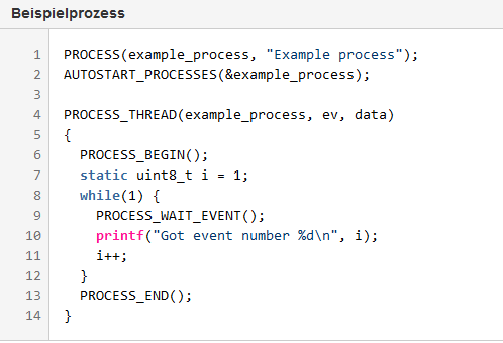
\includegraphics[width=0.9\textwidth]{Beispielprozess.png}
	\label{Beispielprozess}
\end{figure}
In Zeile 1 wird der Prozess initialisiert und in Zeile 2 automatisch beim Boot von Contiki gestartet. Zeile 4 beinhaltet die Deklaration. So k\"onnen andere Prozesse diesem Prozess Events (mit oder ohne Daten) schicken, auf die unser Beispielprozess mit ev und data zugreifen kann. Zeile 6 kennzeichnet den Beginn der tats\"achlichen Ablauflogik. Code \"uber dieser Zeile wird bei jedem Prozessaufruf ausgef\"uhrt, dies wird jedoch in den meisten F\"allen nicht ben\"otigt. Zeile 13 schlie{\ss}lich beendet den Prozess und entfernt ihn aus der Prozess-Liste des Kernels. In diesem Beispiel wird die Zeile jedoch nie erreicht, sodass er Prozess immer wieder aufgerufen wird, bis er von einem anderen Prozess beendet wird.
Wichtige Funktionen in Prozessen:
\begin{itemize}
\item PROCESS\_WAIT\_EVENT()- Wartet auf ein beliebiges Event, bevor die Ausf\"{u}hrung fortgesetzt wird
\item PROCESS\_WAIT\_EVENT\_UNTIL(condition) - Wartet auf ein beliebiges Event, setzt die Ausf\"{u}hrung aber nur fort, wenn die Bedingung erf\"{u}llt ist
\item PROCESS\_WAIT\_UNTIL() - Wartet, bis die Bedingung erf\"ullt ist. Muss den Prozess nicht zwangsl\"{a}ufig anhalten
\end{itemize}
Prozesse k\"onnen \"uber Events (siehe Events) oder Polling-Anfragen kommunizieren.  Polls sind Events mit hoher Priorit\"at und k\"onnen genutzt werden, um den angerufenen Prozess so schnell wie m\"oglich auszuf\"uhren. Sie
sind besonders bei der Abarbeitung von Hardware-Interrupts wichtig, da Interrupts-Handler keine Events, sondern nur
Polling-Anfragen absetzten d\"urfen \cite[S. 7]{Walter:2010}.
	
	% Chapter 5 Teilbericht Simulation
	\clearpage
	\ohead[Teilbericht Simulation]{Teilbericht Simulation}
	\chead[Uni Oldenburg]{Uni Oldenburg}
	\ihead[PG FAISE]{PG FAISE}
	\setheadtopline{1pt}
	\setheadsepline{0.5pt}
	\ofoot[Endbericht]{Endbericht}
	\cfoot[\pagemark]{\pagemark}
	\ifoot[30. September 2014]{30. September 2014}
	\setfootsepline{0.5pt}
	\setfootbotline{1pt}
	\section{Teilbericht Simulation}
Der Teilbericht der Simulationsgruppe beschreibt die entwickelte Simulationssoftware von der Anforderungsanalyse über die Implementierung hin zum Testen und Validieren. Im Lastenheft werden, die für die Simulation vorgegebenen Anforderungen beschrieben. Grundlegende Designentscheidungen, die vor dem Erstellen der Anforderungen getroffen werden müssen, sind ebenfalls Teil der nachfolgenden Kapitel. In dem darauffolgenden Kapitel werden die jeweiligen Systemkomponenten konzipiert. Anschließend soll beschrieben werden, wie die Komponenten implementiert wurden. Das letzte Kapitel dieses Teilberichts beinhaltet Testen und Validieren des entwickelten Systems.
\subsection{Lastenheft}
In der Teilgruppe Simulation soll auf Basis des Ablaufkonzepts (Vgl.Abschnitt\ref{AL}) ein Softwaretool entwickelt werden, das es erlaubt, einen automatisierten Materialfluss auf Basis von FTS zu simulieren, ohne dabei an die zahlenmäßigen Beschränkungen des physischen Systems gebunden zu sein. Vonseiten des Auftraggebers wurde ein Lastenheft vorgegeben, das die gewünschten Kernfunktionalitäten der Software beschreibt. Es enthält folgende Anforderungen:
\begin{enumerate}
\item \textbf{Akteure}: Die virtuellen Akteure ähneln in ihrem Verhalten und Eigenschaften (Geschwindigkeit, Dauer einer Paketübergabe etc.) den echten Objekten aus dem physischen System (Volksbots und Rampen).
\item \textbf{Ablauf}: Der in Abschnitt 4.1 beschriebene Ablauf, wird durch die Software simuliert. 
\item \textbf{Visualisierung}: Die Zustände der Akteure werden dynamisch visualisiert. Wird beispielsweise die Anzahl der Pakete auf einer Rampe um eins erhöht, dann soll dies unmittelbar in der Anzeige visualisiert werden.
\item \textbf{Generierung von Aufträgen}: Eingehende und ausgehende Transportaufträge können erstellt und ausgeführt werden. 
\item \textbf{Einstellungen}: Parameter der Simulation (Anzahl und Art der Akteure, Anzahl der Aufträge etc.) können vom Nutzer vor dem Starten der Simulation angepasst werden.
\item \textbf{Statistiken}: Es werden wichtige Daten geloggt, um am Ende eines Simulationslaufs aussagekräftige Analysen  machen zu können.
\end{enumerate}
\subsection{Grundlegende Designentscheidungen}
Vor der Entwicklung der Simulationssoftware mussten grundlegende Designentscheidung getroffen werden. Zum einen musste entschieden werden, ob die Software auf Basis eines vorhanden Tools oder komplett neu entwickelt werden sollte. Auch musste zwischen Desktop- und Webanwendung entschieden werden und ob die jeweilige Alternative mit oder ohne Zuhilfenahme eines Frameworks implementiert wird. In den nachfolgenden Abschnitten werden die getroffenen Designentscheidungen begründet.
\subsubsection{Eigenentwicklung}
Im Vorfeld der Entwicklung wurde der Teilgruppe Simulation das Player/Stage Tool als Alternative zu einer kompletten Neuentwicklung einer Software vorgeschlagen. Das Tool beinhaltet zum einen die Komponente Player, die eine Hardware Abstraktionsschicht darstellt. Mit dieser Komponente kann mit Robotern, wie beispielsweise einem Volksbot, interagiert werden, ohne dass technische Details der Komponenten (Laserscanner, Motor etc.) bekannt sein müssen. Auf Basis von selbstgeschriebenem Code können Roboter gesteuert werden. Die Komponente Stage horcht auf die Befehle, die Player ausführt und visualisiert diese in einem eigenen Graphical User Interface. Jedoch kann Stage auch ohne Hardware benutzt werden, indem man über Konfigurationsdateien ein eigenes Szenario erstellt und die virtuellen Roboter über den eigenen Code steuert. Somit bietet das Tool die Möglichkeit, eine Simulation mit Robotern zu erstellen und das gewünschte Verhalten der Roboter über eigenen Code abzubilden. Auch muss die Visualisierung nicht selbst entwickelt werden (Vgl.\cite{plstg}). 
\\\\
Dennoch wurde eine Eigenentwicklung der Nutzung des Tools vorgezogen. Die Benutzeroberfläche von Stage bietet die Möglichkeit, die Anzahl der Roboter und das Layout eines Szenarios über die entsprechenden Konfigurationsdateien einzustellen (Vgl.\cite{plstg}). Jedoch gibt es beispielsweise keine Möglichkeit Aufträge zu erstellen bzw. zu simulieren oder Statistiken anzuzeigen. Somit ist die Entwicklung einer eigenen Benutzeroberfläche unumgänglich. Das bedeutet, dass die Stage Oberfläche über eine eigene Benutzeroberfläche gesteuert werden muss. Somit hätte man eine Trennung zwischen Visualisierung und Konfiguration eines Szenarios, was die Benutzerfreundlichkeit erheblich beeinträchtigt, da ein Nutzer den Durchlauf einer Simulation über zwei Benutzeroberflächen hinweg verfolgen müsste. Die Entwicklung eines eigenen Systems bietet somit erheblich mehr Benutzerfreundlichkeit und ermöglicht es, alle Anforderungen an das Interface in einer Benutzeroberfläche zu integrieren. 
\subsubsection{Entwicklung einer Webanwendung}\label{sec:Entwicklung einer Webanwendung} 
Die Software soll als Webanwendung implementiert werden. Gegenüber einer Desktopanwendung bietet eine Webapplikation folgende Vorteile:
\begin{itemize}
\item Das System ist plattformunabhängig und kann somit auf jedem Rechner, der über einen Webbrowser verfügt, ausgeführt werden.
\item Die Software muss nicht lokal installiert werden und kann direkt genutzt werden.
\item Werden Änderungen an der Software vorgenommen, sind diese direkt verfügbar, da Updates über den Webserver eingespeist werden. Die Software ist somit immer auf dem aktuellsten Stand. 
\end{itemize}
\subsubsection{Umsetzung durch GWT}\label{GWT} 
Die Entwicklung der Webanwendung sollte mithilfe eines Frameworks erfolgen, das es erlaubt, den Code sowohl für die Client- als auch für die Serverseite in einer Programmiersprache zu entwickeln. Außerdem sollte das Framework Schnittstellen bieten, um asynchrone Kommunikation und Push-Dienste zu nutzen, ohne sich um die exakten Details kümmern zu müssen. Ausgewählt wurde das Google Web Toolkit (GWT). GWT ist ein von Google entwickeltes Framework zur Erstellung von Webanwendungen. Der Java-Code für den Client wird von dem GWT Compiler in den entsprechenden Javascript- und HTML-Code übersetzt. Somit kann die Entwicklung sowohl für Client als auch für den Server auf Basis von Java erfolgen. Zudem entfällt die Anpassung des Javascript-Codes für die verschiedenen Browser, da GWT beim Kompilieren automatisch für jeden Browser eine lauffähige Version erzeugt. Weiterhin besitzt GWT  eine RCP-Schnittstelle für die Kommunikation zwischen Client und Server und lässt sich um Komponenten erweitern, um Daten vom Server zum Client zu pushen (Vgl.\cite{gwt}). Somit erfüllt GWT sämtliche an ein Framework gestellte Anforderungen. Weitere Alternativen wurden nicht in Betracht gezogen, da drei von fünf Mitgliedern der Teilgruppe Simulation bereits positive Erfahrungen mit GWT gemacht haben und die anderen Mitglieder somit schnell einarbeiten konnten. 
\subsection{Konzeption der Systemkomponenten}
In diesem Abschnitt wird die Konzeption der Gesamtarchitektur als auch der einzelnen Systemkomponenten beschrieben, die im Rahmen der Sprints erarbeitet wurde. Die Konzeption beinhaltet zum einen die Anforderungen, als auch die daraus abgeleiteten Implementierungsvorgaben.
\newpage
\subsubsection{Gesamtarchitektur}\label{GA} 
Wie in Kapitel \ref{sec:Entwicklung einer Webanwendung} beschrieben, soll die Software als Webanwendung realisiert werden. Eine Webanwendung erfordert eine Client-Server Architektur. Abbildung \ref{Gesamtarchitektur} beschreibt die wesentlichen Komponenten des Systems und wie diese sich auf die Client- und Serverseite verteilen. Basis der Anwendung ist der Webserver, der die Basiskomponenten des Systems hosted. Zum einen stellt er die Laufzeitumgebung für Webanwendung und Datenbank bereit. Die Datenbank wird benötigt, um Daten, wie beispielsweise erstellte Szenarien, persistent zu speichern. Aus der Webanwendung heraus kann auf die Datenbank lesend und schreibend zugegriffen werden. In die Webanwendung soll ein Multiagentensystem (MAS) eingebettet werden. Ein MAS ist ein Netzwerk aus Softwareagenten. Softwareagenten sind Softwareeinheiten, die in  der Lage sind, Aufgaben selbstständig durchzuführen (Vgl.\cite{mas}). Mithilfe des MAS können die im Ablaufszenario beschriebenen Aktionen softwareseitig auf die Akteure abgebildet werden.
\\\\
Der Webserver beinhaltet die Logik des Systems. Auf dem Client soll die Visualisierung erfolgen und der Nutzer soll das Starten einer Simulation initiieren können. Das System soll von einem Webbrowser aus aufrufbar sein, in dem die Ergebnisse der serverseitigen Prozesse dargestellt werden. 

\begin{figure}[h!]
	\centering
		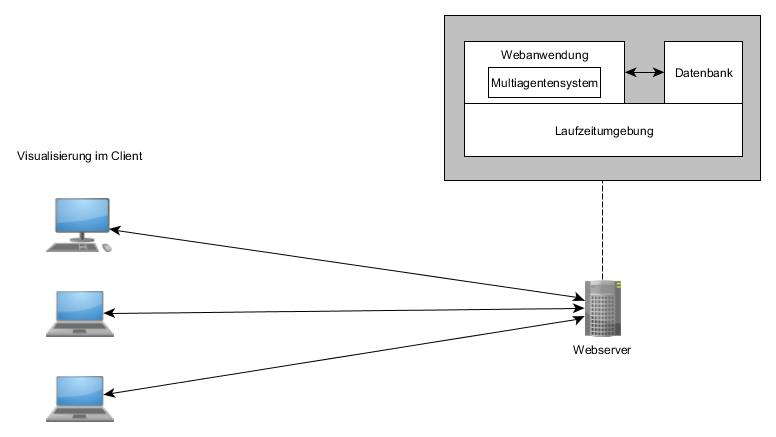
\includegraphics[width=0.8\textwidth]{grobarchitektur.jpg}        
		\caption{Gesamtarchitektur}
	\label{Gesamtarchitektur}
\end{figure} 
\newpage
\subsubsection{Konzeption der Benutzeroberfläche}
Die Benutzeroberfläche soll einem Nutzer die Möglichkeit bieten, auf sämtliche Funktionalitäten, die für die Durchführung eines Simulationsdurchlaufs relevant sind, zuzugreifen. Abbildung \ref{GUI} zeigt den schematischen Aufbau der Gui anhand eines Mockups. Die Menüleiste beinhaltet drei Menu Items: Simulation, Auftragsliste und Statistiken. Über die Items Simulation und Auftragsliste sollen erstellte Szenarien und Auftragslisten geladen und gespeichert werden können. Außerdem soll eine Simulation gestartet werden können. Das Statistik Item erlaubt den Zugriff auf Statistiken, die für einen Durchlauf generiert wurden. Links unter der Menüleiste befindet sich die Auftragsliste, über die Aufträge generiert und angezeigt werden können. Darunter befindet sich der Bereich, der für die Modellierung eines Szenarios relevant ist. Es sollen Rampen, Fahrzeuge und Wände als Modellelemente auswählbar sein und in der Zeichenfläche platziert werden können. Die Zeichenfläche selber befindet sich rechts unter der Menüleiste. Dort werden die Aktionen der Akteure, wie z.~B. Aufladen eines Pakets, visualisiert. Das unterste Element enthält eine Debug-Konsole, in der serverseitige Aktionen dargestellt werden können, die nicht in der Zeichenfläche dargestellt werden sollen. 
\begin{figure}[h!]
	\centering
		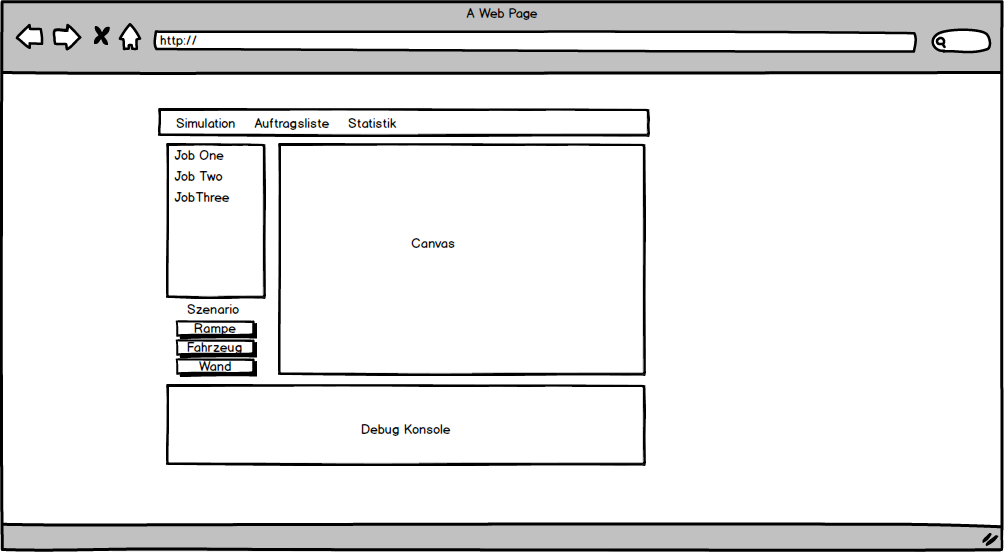
\includegraphics[width=0.8\textwidth]{Mockup.png}        
		\caption{Schematischer Aufbau der Benutzeroberfläche}
	\label{GUI}
\end{figure}
\subsubsection{Generierung von Aufträgen} \label{Generierung von Aufträgen}  
Die Simulationssoftware soll ein Umschlagslager simulieren. Das bedeutet, dass Pakete in das Lager geliefert, zwischengelagert und an den Ausgangsrampen wieder abgeholt werden, wenn ein bestimmtes Paket angefragt wird (Vgl.\ref{Einsatzszenario}). Das bedeutet, dass eine Unterscheidung getroffen werden muss zwischen einem physischen Paket und einer Nachfrage nach einem bestimmten Paket, die ein Ausgang stellt. Deshalb soll zwischen eingehenden und ausgehenden Aufträgen unterschieden werden. Es soll möglich sein, eine festgelegte Anzahl an Aufträgen zufällig über die Gui zu generieren. Es muss sichergestellt werden, dass die Menge an generierten eingehenden und ausgehenden Aufträgen in einem bestimmten Verhältnis zueinander stehen und ausgehende Aufträge für vorhandene Pakete generiert werden. So wird sichergestellt, dass Pakete nicht nur im Zwischenlager landen, sondern auch am Ausgang nachgefragt werden.
\subsubsection{Anforderungen an ein Multiagenten-Framework}
Um ein Umschlagslager und die darin enthaltenden Akteure (Rampen und Fahrzeuge) zu simulieren, soll ein Multiagentensystem eingesetzt werden (Vgl.\ref{GA}). Zur Erstellung eines MAS soll ein Framework verwendet werden, dass die nachfolgenden Anforderungen erfüllt: Das Framework muss das Erstellen von verschiedenen Agententypen ermöglichen, um die Akteure mit ihren spezifischen Aufgabenstellungen simulieren. Agenten müssen in der Lage sein, untereinander Nachrichten auszutauschen und auf bestimmte Nachrichten oder Ereignisse mit definierten Verhaltensweisen zu reagieren. Weiterhin sollen die Aktionen der Agenten denen der realen Akteure hinsichtlich der Dauer ähneln. Außerdem muss das Framework Aktionen von verschiedenen Agenten parallel ausführen können, damit beispielsweise das gleichzeitige Fahren mehrerer Fahrzeuge möglich ist.
\subsubsection{Benötigte Agententypen}
Sowohl Rampen als auch Fahrzeuge müssen verschiedene Aktionen durchführen. Dazu gehören u.~a. das Befördern von Paketen, die Vergabe von Aufträge, Durchführung von Auktionen usw. Würde man alle Aufgaben, die ein Akteur durchführen muss, in einem Agenten bündeln, so wäre ein solcher Agent nur schwer wartbar und es könnten abhängig vom Agenten-Framework Probleme bei der Parallelisierung von Aktionen auftreten. Es bietet sich an, die erforderlichen Aufgaben eines Akteurs auf mehreren Agenten zu verteilen. Durch die Modularisierung kann die Entwicklung des Systems parallelisiert werden und Änderungen an einem Agenten haben geringere Auswirkungen auf das Gesamtsystem. Die Wartbarkeit des Systems erhöht sich. Für das zu entwickelnde System wurden die folgenden vier Agententypen konzipiert:  
\begin{itemize}
\item Paketagent: Verwaltung der Paketdaten
\item Orderagent: Ermittlung von Zielrampen und Zuweisung von Zielen (Wird nur bei Rampen benötigt)
\item Routingagent: Durchführung von Auktionen und Berechnung von möglichen Pfaden
\item Plattformagent: Durchführung physischer Aktionen (Fahren, Aufladen von Paketen etc.)
\end{itemize}
\subsubsection{Kommunikation zwischen den Agenten}
Die zu entwickelnde Software soll die in Abschnitt \ref{AL} beschriebenen Abläufe umsetzen. Die Aufgaben der verschiedenen Akteure müssen auf die Agenten verteilt werden. Die entworfenen Kommunikationsschritte der Agenten sollen für den Fall beschrieben werden, dass ein Eingang Ausgänge und Zwischenlager fragt, ob ein Paket entgegengenommen werden kann. Anhand des Beispiels soll die Verteilung der Aufgaben auf die unterschiedlichen Agenten skizziert werden.
\begin{enumerate}
\item Trifft ein Paket ein, verlangt der Paketagent vom Orderagenten eine Destination für das entsprechende Paket.
\item Der Orderagent einer Eingangsrampe fragt die Orderagenten der Ausgangs- und Zwischenrampen.
\item Die Orderagenten prüfen im Abgleich mit ihren Paketagenten, ob Platz frei ist (Zwischenrampe) oder die Paket-ID benötigt wird (Ausgang). Anschließend antworten sie dem Orderagenten am Eingang.  
\item Wurde ein Ziel für das Paket gefunden, soll der Orderagent den Start einer Auktion initiieren, indem er den Routingagenten benachrichtigt. 
\item Der Routingagent verlangt eine Aufwandsschätzung von allen Routingagenten der Fahrzeuge.
\item Der Routingagent eines Fahrzeugs berechnet eine Aufwandsschätzung anhand seiner Position und antwortet dem Routingagenten der Rampe. Fährt der Volksbot oder nimmt er an einer anderen Auktion teil, so wird -1 als Aufwandsschätzung zurückgeschickt.
\item Der Routingagent einer Rampe wählt, sofern vorhanden, den Bot aus, der den geringsten Aufwand benötigt, um ein Paket abzuholen und weist ihm den Auftrag zu.
\item Der Plattformagent fährt zu der jeweiligen Eingangsrampe und lädt das Paket auf. Dies geschieht durch einen Nachrichtenaustausch mit dem jeweiligen Plattformagenten der Rampe, der die Paketdaten übergibt. Das Fahren zur Zielrampe und das Abladen des Pakets erfolgt analog. 
\end{enumerate}
\subsubsection{Konzeption des Pathfindings}
Die Fahrzeuge eines Szenarios holen die Pakete von den Eingangsrampen ab und liefern sie zu den jeweiligen Zielrampen. Da der Anwender nicht selbst in den Simulationsablauf eingreifen möchte, um mögliche Pfade von Hand anzugeben (für den Transport der Pakete), wurde ein Pathfinding-Konzept entwickelt. Zunächst wird die Startposition in der Karte ermittelt. Anschließend wird im Uhrzeigersinn jede benachbarte Kachel ermittelt, bei der es sich um kein Hindernis handelt. Sollte eine gefundene Kachel noch nicht bearbeitet worden sein, wird ihr ein Wert zugewiesen, der  Aufschluss darüber gibt, wie weit die anliegende Kachel von der aktuellen entfernt ist (notwendig u.a. für diagonales Fahren). Zudem wird der aktuelle Gridwert erhöht und der neuen Kachel zugewiesen. Sollte eine Kachel mehrmals bei der Zuweisung ermittelt werden, wird der kleinste gefundene Wert in der Kachel beibehalten, da ein kleinerer Wert einen kürzeren Pfad repräsentiert.
\\\\
Nachdem alle Kacheln auf der Karte mit Werten versehen wurden, wird vom Endpunkt aus ein möglicher Weg zum Startpunkt zurück berechnet. Dabei wird der Wert in der Endkachel genommen und mit den benachbarten Kacheln verglichen. Sollte mindestens eine Kachel eine kleinere Wertigkeit aufweisen, wird somit erkannt, dass es sich um einen kürzeren Weg zur Startposition handelt. Sollten mehrere angrenzende Kacheln diese Eigenschaft aufweisen, wird zufällig eine von ihnen ausgewählt. Während dieser Rückwärtssuche (von der Endposition zur Startposition)
wird bis die Startposition wieder gefunden wurde, jede Position der ausgewählten Kacheln gespeichert. Nachdem der Startpunkt gefunden wurde, müssen sämtliche gefundenen Positionen in der Liste getauscht werden (Punkte an Ende der Liste starten nun am Anfang der Liste und umgekehrt).
Dies ist notwendig, da das Fahrzeug diese Positionen abfahren soll, jedoch liegen die Punkte in umgekehrter Reihenfolge vor, weil der Pfad von der Endposition zur Startposition ermittelt wird.

\subsubsection{Konzeption der Statistiken}\label{konzept_statistik}
Um eine Vergleichbarkeit zwischen verschiedenen Ausführungen einer Simulation zu schaffen, müssen Statistiken berechnet werden, die einfache Kennzahlen berechnet, mithilfe dessen man die Simulationen bewerten und vergleichen kann. Als wichtigen Kennzahlen wurde hier die Auslastung der Volksbots und die Durchlaufzeit der Pakete in der Simulation gewählt.

\begin{enumerate}
	\item \textbf{Auslastung der Volksbots}: Die Statistik erhält immer dann Daten, wenn ein Bot einen seinen Status wechselt ("Arbeitend" <-> "Wartend"). Daraufhin muss das Intervall berechnet werden, welches zwischen dem jetzigen und dem letzten Statuswechsel lag. Dieses sagt dann aus, wie lange der Volksbot sich in dem jeweiligen Status befand. Diese Daten werden dann über alle Bots aggregiert und ins Verhältnis gesetzt und visuell aufbereitet abrufbar.
	\item \textbf{Paketdurchlaufzeit}: Die Statistik der Paketdurchlaufzeit muss immer dann benachrichtet werden, sobald ein neuer Auftrag in die Simulation eintritt. Dieser Zeitpunkt wird im dann festgehalten und sobald dieses Paket dann die Simulation verlässt (Abtransport eines Pakets) wird das Intervall zwischen Eintritt und Austritt des Pakets berechnet. Der neue Wert wird dann in einem Liniendiagramm vermerkt. Das Liniendiagramm bietet die Möglichkeit, zu erkennen wie sich die Paketdurchlaufzeit über die Ablaufzeit der Simulation verändert.
\end{enumerate}

Für die Kapselung der Aufgaben, die zur Datenhaltung und Berechnung der Statistiken nötig sind, wird eigens ein Statistik-Agent in der Simulation eingeführt. Dieser soll zu bestimmten Ereignissen informiert werden. Er sorgt dafür, die Daten zu aggregieren und in aufbereiteter Form der UI bereitzustellen. Des weiteren informiert er die UI, sobald neue Daten bereitstehen.

\subsubsection{Interaktion der Komponenten} \label{Interaktion der Komponenten}
Durch das Zusammenspiel der Systemkomponenten soll eine Simulation durchgeführt werden. Die Aufträge müssen entsprechend ihrer Zeiten an den Server geschickt werden. Dies soll clientseitig durch einen Timer durchgeführt werden. Abbildung \ref{Int} zeigt den Ablauf und die Komponenten, die für das Starten einer Simulation erforderlich sind: 
\begin{enumerate}
\item Ein potenzieller Nutzer startet eine Simulation über die Benutzeroberfläche.
\item Der Server wird durch die GUI informiert, dass die Simulation gestartet werden soll.
\item Der Server startet das Multiagentensystem.
\item Der Server meldet dem Client den Start des MAS.
\item Der Client weiß nun, dass die Agenten bereit sind, Aufträge entgegenzunehmen und startet den Timer für die Jobliste.
\item Die Aufträge werden gemäß ihrer Startzeit an den Server geschickt.
\item Der Server leitet die Aufträge an das MAS weiter
\item Die Daten über sichtbare Zustandsveränderungen werden an den Client geschickt und dort in der GUI visualisiert.
\end{enumerate}

\begin{figure}[h!]
	\centering
		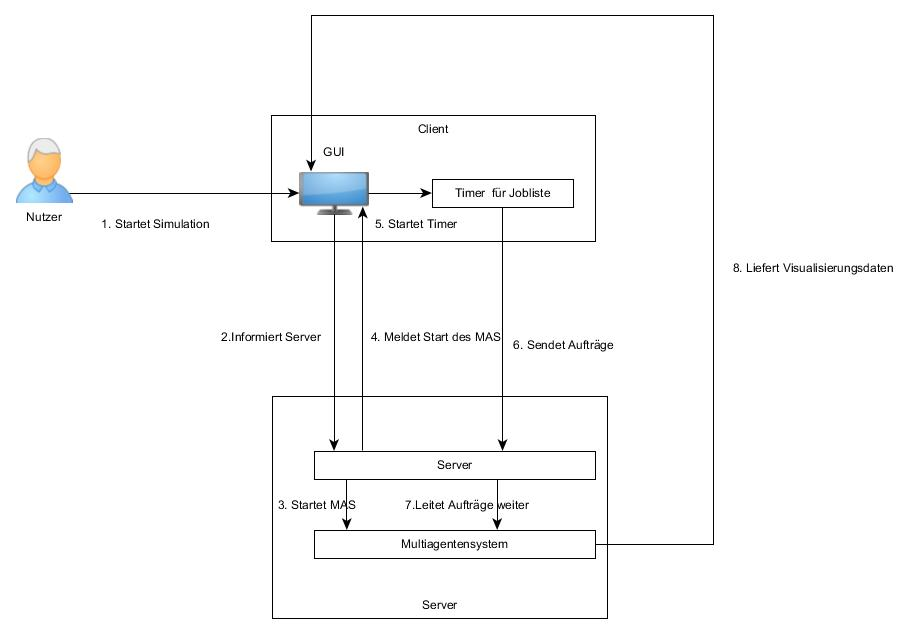
\includegraphics[width=0.8\textwidth]{Interaktion.jpg}        
		\caption{Interaktion der Systemkomponenten}
	\label{Int}
\end{figure}

\newpage
\subsection{Implementierung der Systemkomponenten}
Inhalt diesen Abschnitts ist die Implementierung der zuvor konzipierten Systemkomponenten. Zum einen soll die Auswahl von Technologien und Frameworks zur Umsetzung beschrieben sowie die Funktionalität des Systems auf technischer Ebene dargestellt werden.
\subsubsection{Implementierte Gesamtarchitektur}
Abbildung \ref{GAI} zeigt die konkrete Gesamtarchitektur des Systems, die durch die Auswahl von Umsetzungstechnologien entstanden ist. Die Webanwendung soll, wie bereits in Abschnitt \ref{GWT} beschrieben, durch das GWT Framework implementiert werden. Der Code für Server und Client, der für Visualisierung, Client-Server Kommunikation u.~ä., benötigt wird, wird durch GWT-Bilbiotheken bereitgestellt. Eingebettet in den serverseitigen Code wird das Multiagentensystem, das mithilfe des Java Agent Development Framework (JADE)\footnote{\cite{jade}} implementiert wurde. Als Datenbankmanagementsystem wurde PostgreSQL ausgewählt. Die Applikation wird durch den internen Jetty Server von GWT gehostet, der die Java Laufzeitumgebung und das GWT Software Development Kit ebenfalls bereitstellt. Die Anwendung kann im Produktivmodus prinzipiell auf jedem Java-fähigen Webserver aufgesetzt werden.  
\begin{figure}[h!]
	\centering
		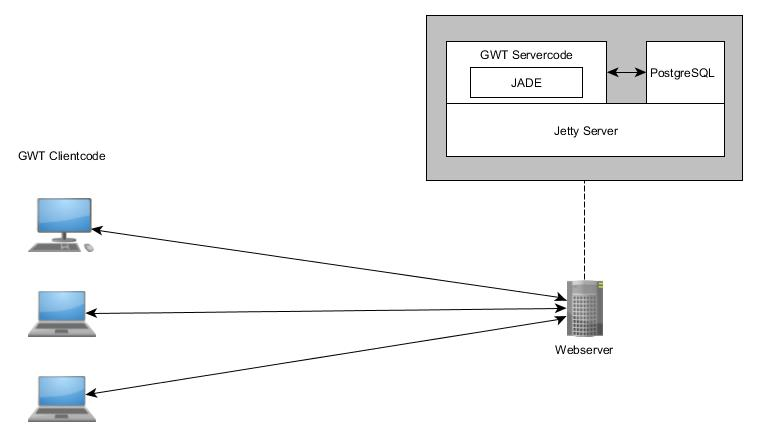
\includegraphics[width=0.8\textwidth]{architekturSimu.jpg}        
		\caption{Implementierte Gesamtarchitektur}
	\label{GAI}
\end{figure}
\subsubsection{Benutzeroberfläche}
Die Implementierung der Benutzeroberfläche erfolgt durch die Klassen Mainframeview und Mainframepresenter. Die View beinhaltet die graphischen Elemente und der Presenter ist für die Programmlogik, wie das Hinzufügen von Listenern oder das Senden von Daten an den Server verantwortlich. Die Benutzeroberfläche ist in die fünf Bereiche Menüleiste, Auftragsliste, Modellelemente, Zeichenfläche und Debugkonsole unterteilt. In der Auftragsliste werden eingehende und ausgehende Aufträge mit ihrer Startzeit, ihrer Paket-ID und ihrem jeweiligen Ziel gelistet. Die Auflistung ist nicht chronologisch, sondern anhand der ID geordnet. Einzelne Aufträge können über einen Button in der vierten Spalte entfernt werden. Eine beliebige Anzahl an Aufträgen kann generiert werden. Der Bereich Modellelemente enthält Rampen, Fahrzeuge und Wände, die per Drag an Drop auf der Zeichenoberfläche platziert werden können. Im untersten Bereich befindet sich die Debugkonsole. 
\begin{figure}[h!]
	\centering
		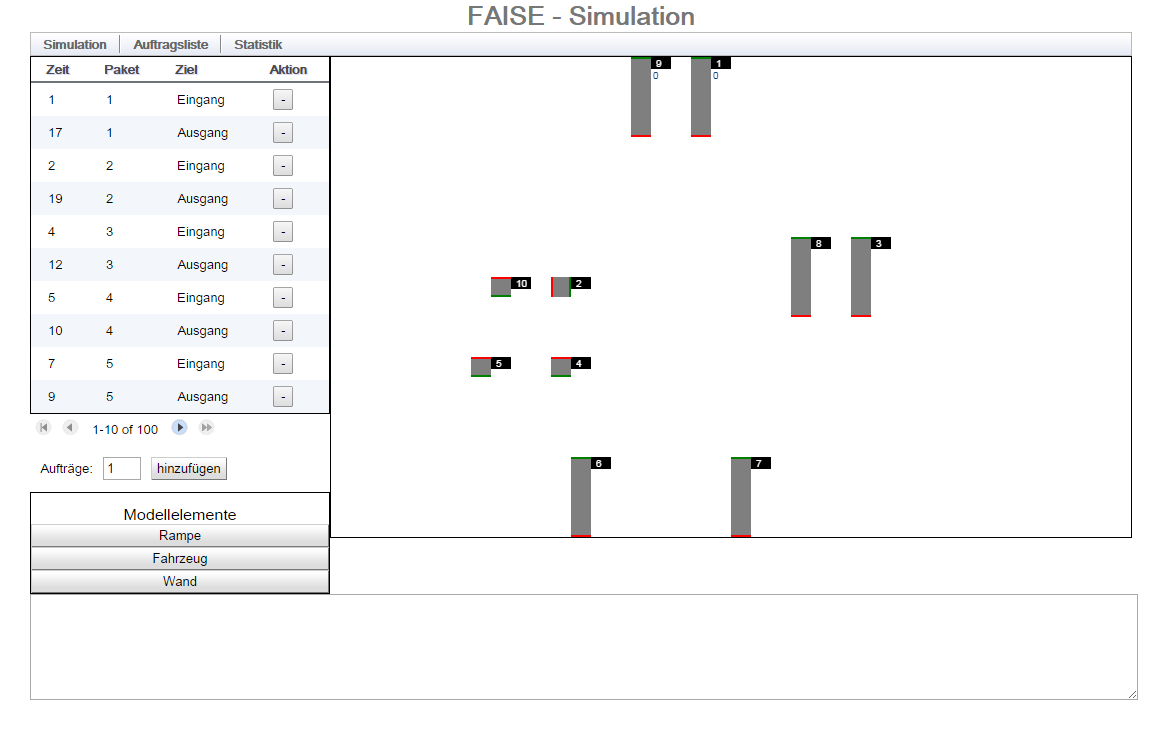
\includegraphics[width=0.8\textwidth]{Gui.PNG}        
		\caption{Benutzeroberfläche}
	\label{GUIIMPL}
\end{figure}
\subsubsection{Generierung von Aufträgen}
Abbildung \ref{AGEN} zeigt die Methode addRandomJobs mit deren Hilfe zufällig eingehende und ausgehende Aufträge generiert werden. Für jeden zu generierenden Auftrag wird in der Variable destinationID zufällig festgelegt, ob es sich, um einen eingehenden oder ausgehenden Auftrag handelt.
Eingehende und Ausgehende Aufträge treten mit gleicher Wahrscheinlichkeit auf. Der Wert Null steht für einen eingehenden und minus Eins für einen ausgehenden Auftrag. In der Variable Timestamp wird die Zeit für den Auftrag festgelegt. Jeder Auftrag beginnt eine Sekunde später als der vorhergehende. Die Zeiten können prinzipiell beliebig angepasst werden. Die ID eines eingehenden Auftrags wird durch eine Variable der Klasse Joblist generiert, die um eins inkrementiert wird. Die IDs der ausgehenden Aufträge werden ebenfalls zufällig generiert, jedoch wird sichergestellt, dass ein ausgehender Auftrag für ein schon vorhandenes Paket generiert wird (Vgl. Abschnitt\ref{Generierung von Aufträgen}).
\\\\  
\begin{figure}[h!]
	\centering
		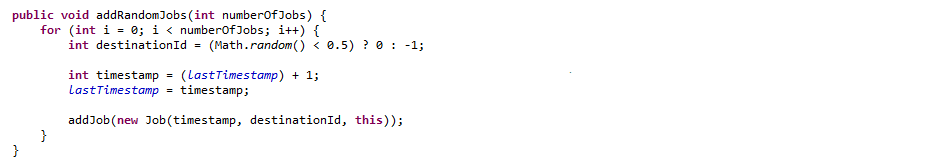
\includegraphics[width=1\textwidth]{Auftragsgenerierung.PNG}        
		\caption{Auftragsgenerierung}
	\label{AGEN}
\end{figure}
\\\\
\subsubsection{Auswahl eines Multiagenten-Frameworks}
Das Java Agent Development Framework wurde genutzt, um ein Netzwerk aus verschiedenen Agenten zu implementieren. Jade erlaubt das Erstellen von verschiedenen Agenten. Agenten werden als Java-Klasse implementiert, die von der vordefinierten Klasse Agent erbt. Die Aktionen, die ein Agent ausführen soll, werden durch Behaviours implementiert, die ebenfalls Klassen sind. Um die Anzahl an Klassen zu reduzieren, wurden die Behaviours als interne Klassen in die Agenten eingefügt. Jade ermöglicht die Kommunikation zwischen den Agenten durch ein vordefiniertes Nachrichtensystem. Nachrichten können sowohl gezielt an einen Agenten adressiert oder an alle Agenten verschickt werden. Die Agenten können in Echtzeit miteinander kommunizieren und mehrere Agenten können parallel Aktionen ausführen, da jeder Agent in einem eigenen Thread läuft (Vgl.\cite{jadetwo}). 
\subsubsection{Implementierte Agententypen}
Implementiert wurden sieben verschiedene Agententypen. Jede Rampe besitzt jeweils einen Paket-, Order-, Routing- und Plattformagenten. Ein Fahrzeug besitzt einen Paket-, Routing- und Plattformagenten. Die Routing- und Plattformagenten wurden für Fahrzeuge und Rampen durch unterschiedliche Agenten implementiert, um die Anzahl an Behaviours pro Agent zu reduzieren und den Code übersichtlicher zu gestalten und unnötigen Speicherverbrauch zu vermeiden. Damit ein Agent weiß, welchem Szenario und welchem Akteur er zugeordnet ist, werden Szenario und Conveyor als Referenz übergeben \footnote{Der genaue Ablauf der Initialisierung wird in Abschnitt \ref{Interaktion der Komponenten} beschrieben}. Neben den genannten Agenten war es notwendig, einen Jobagent zu implementieren, der die Übergabe eines Pakets zu simulieren, die im phyischen System durch einen Menschen geschieht. Außerdem werden ausgehende Aufträge durch den Jobagent an die Ausgangsrampen übermittelt. Es wurde anders als im physischen System darauf verzichtet für jedes Paket einen Paketagenten zu erzeugen, da die Synchronisation der Paketdaten ansonsten einen zu großen Synchronisationsaufwand erfordert hätte, was wiederum die Anzahl der Nachrichten zwischen den Agenten erhöht und fehleranfälliger ist.
\subsubsection{Kommunikation zwischen den Agenten}
In den nachfolgenden Abschnitten soll die Kommunikation zwischen den Agenten, die implementiert wurde, anhand von Sequenzdiagrammen beschrieben werden. Dabei werden folgende Anwendungsszenarien durchlaufen:
\begin{itemize}
\item Jobzuweisung an Ein- und Ausgänge.
\end{itemize}

\paragraph{Jobzuweisung an Ein- und Ausgänge} \label{Jobagent}
Abbildung \ref{Job} zeigt die Jobzuweisung an die Ein- und Ausgangsrampen durch den Jobagent. Bevor die Jobzuweisung beginnt, wird die Simulation durch den Client gestartet. Neben dem Jobagent, den Plattformagenten der Rampen und dem Paketagenten ist das Servlet AgentPlattformServiceImpl an der Kommunikation beteiligt. Auf die Aspekte der Client-Server Kommunikation wird in Abschnitt  \ref{Interaktion der Komponenten} genauer eingegangen. Das Diagramm zeigt folgenden Ablauf:
\begin{itemize}
\item Die Simulation wird aus dem Browser heraus gestartet und das Servlet wird benachrichtigt.
\item Das Servlet startet die Agentenplattform und initialisiert die Agenten, einschließlich dem Jobagent. 
\item Der Jobagent startet einmalig eine Anfrage an die Plattformagenten der Rampen, um die IDs und die Anzahl der Ein- und Ausgänge zu erfragen, die für die Jobzuweisung nötig sind. 
\item Die Plattformagenten senden ihren Rampentyp an den Jobagent.
\item Der Jobagent besitzt zwei Listen in denen er die IDs, der Ein- und Ausgänge speichert. Anhand des empfangenen Rampentyps, speichert er die ID des Senders in der entsprechenden Liste. Anschließend wird der Client benachrichtigt, dass die Simulation gestartet wurde.
\item Der Client startet den Jobtimer und sendet die Aufträge entsprechend ihrer zeitlichen Reihenfolge an das Servlet.
\item Das Servlet leitet die Aufträge an den Jobagent weiter.
\item Der Jobagent empfängt den Auftrag und sendet eine Nachricht an sich selbst.
\item Je nach Art des Auftrags werden entweder die Eingangs- oder Ausgangsrampen gefragt, ob der Auftrag entgegengenommen werden kann.
\item Die Plattformagenten senden eine Nachricht an ihre Paketagenten, um zu prüfen, ob der Auftrag aufgenommen werden kann. Der Plattformagent wartet auf die Antwort des Paketagenten.
\item Der Paketagent prüft, ob der Auftrag entgegengenommen werden kann und antwortet dem Plattformagent.
\item Der Plattformagent verarbeitet die Anfrage und antwortet dem Jobagent. Läuft der Plattformagent auf einer Ausgangsrampe, so wird automatisch geantwortet, dass Platz verfügbar ist, da ausgehende Aufträge nur IDs repräsentieren, die der Ausgang anfragt. Ein Ausgang kann unbegrenzt IDs anfragen.
\item Der Jobagent wählt unter den Rampen, die einen Auftrag entgegennehmen können, zufällig eine aus und sendet die Auftragsdaten an den Plattformagenten.
\item Der Plattformagent initialisiert mit den Auftragsdaten die Paketdaten und schickt diese an den Paketagenten. Zu beachten ist, dass die Klasse PackageDate sowohl eingehende als auch ausgehende Aufträge repräsentiert.
\item Der Paketagent fügt das Paket einer Liste hinzu.
\end{itemize}   
\begin{figure}[h!]
	\centering
		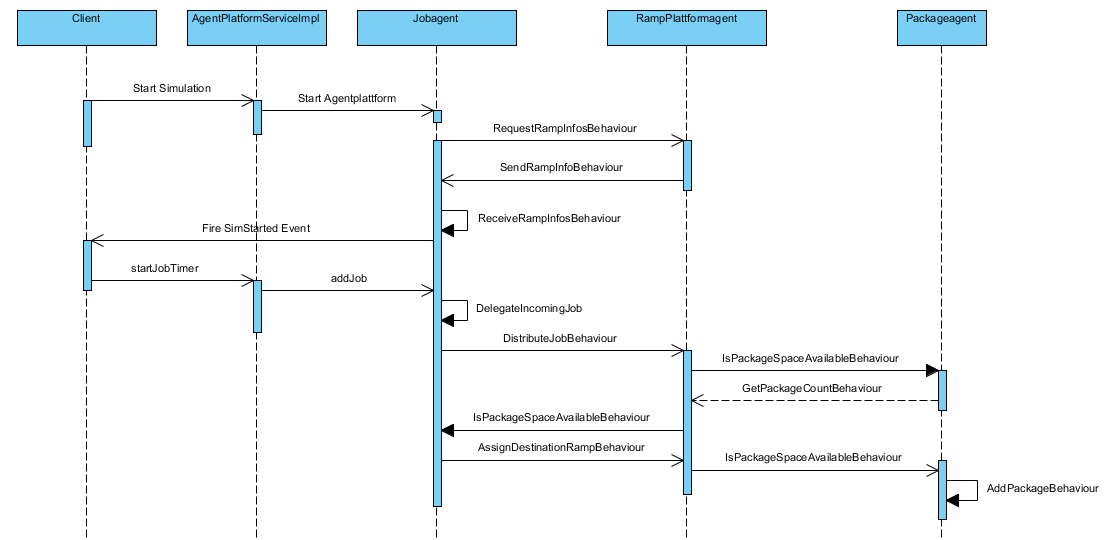
\includegraphics[width=1\textwidth, height=0.6\textwidth]{Jobagent.png}        
		\caption{Jobzuweisung an Ein- und Ausgänge}
	\label{Job}
\end{figure}
\newpage
\paragraph{Eingang fragt Ausgang und Zwischenlager}
Pakete, die am Eingang eintreffen, werden weitergeleitet. Besteht ein Bedarf am Ausgang, so soll das Paket zum Ausgang befördert werden. Ansonsten wird es ins Zwischenlager gebracht. Abbildung \ref{Eingang fragt} zeigt den Nachrichtenaustausch der Agenten, der zur Zielfindung nötig ist:
\begin{itemize}
\item Der Paketagent stellt mithilfe einer Tickerbehaviour zyklisch Anfragen an seinen Orderagenten, um ein Ziel für das vorderste Paket zu bekommen. Bevor der Orderagent benachrichtigt wird, prüft der Paketagent mithilfe der Variable OutgoingJobFlag, ob für das Paket bereits ein Ziel gefunden wurde. Falls nicht, sendet er die Anfrage an den Orderagenten.  
\item Der Orderagent sendet eine Nachricht an alle Orderagenten der Ausgangs- und Zwischenrampen.
\item Der jeweilige Orderagent fragt seinen Paketagenten, ob bereits ein Paket erwartet wird. Dies ist nötig, damit sich nicht mehrere Bots vor einer Rampe blockieren.
\item Der Paketagent prüft anhand der Variable IncomingJobFlag, ob ein Paket erwartet wird und antwortet seinem Orderagenten.
\item Sofern kein Paket erwartet wird, fährt der Orderagent fort und stellt eine erneute Anfrage an seinen Paketagenten, um zu fragen, ob das entsprechende Paket benötigt wird (Ausgang) oder ob Platz frei ist (Zwischenlager).
\item Der jeweilige Orderagent antwortet dem Eingang, ob das Paket entgegengenommen werden kann oder nicht.
\item Der Orderagent des Eingangs speichert die IDs der Rampen, die ein Paket aufnehmen können, wählt unter diesen zufällig eine aus und übermittelt die Daten für Start- und Zielrampe an den Routingagent, damit dieser die Auktion starten kann. Der Orderagent wartet bis die Auktion beendet ist. 
\item Wurde die Auktion erfolgreich durchgeführt, teilt der Orderagent des Eingangs dem Paketagenten der Zielrampe mit, dass sich ein Paket im Anmarsch befindet, damit dieser das IncomingJobFlag setzt.
\item Paketagent antwortet dem Orderagenten, dass das Flag gesetzt wurde.
\item Der Orderagent informiert seinen Paketagent, damit dieser das OutgoingJobFlag setzt.
\end{itemize} 

\begin{figure}[h!]
	\centering
		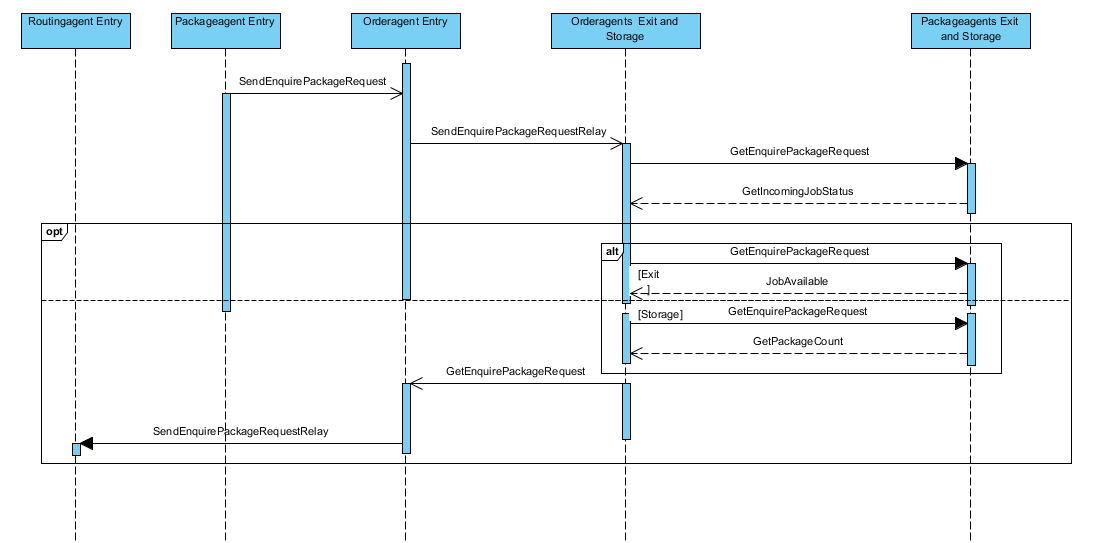
\includegraphics[width=1\textwidth, height=0.6\textwidth]{EingangAusgang.png}        
		\caption{Eingang fragt Ausgang und Zwischenlager}
	\label{Eingang fragt}
\end{figure}
\newpage
\paragraph{Ausgang fragt Zwischenlager}
Pakete, die am Eingang eintreffen und für die noch keine Nachfrage an den Ausgangsrampen besteht, werden ins Zwischenlager gebracht. Damit auch diese Pakete zum Ausgang gelangen, fragt der Ausgang zyklisch im Zwischenlager für die entsprechenden Pakete nach. Abbildung \ref{Ausgang fragt} zeigt den Ablauf im Detail:
\begin{itemize}
\item Der Paketagent des Ausgangs stellt mithilfe einer Tickerbehaviour zyklisch Anfragen an seinen Orderagenten, damit im Zwischenlager geprüft wird, ob ein Paket vorhanden ist, für das eine Nachfrage besteht. Bevor der Orderagent benachrichtigt wird, prüft der Paketagent mithilfe der Variable IncomingJobFlag, ob bereits ein Paket erwartet wird. Falls nicht, sendet er die Anfrage an den Orderagenten.  
\item Der Orderagent sendet eine Nachricht an alle Orderagenten der Zwischenrampen.
\item Der jeweilige Orderagent fragt seinen Paketagenten, ob bereits ein Paket abgeholt wird. Dies ist nötig, damit sich nicht mehrere Bots vor einer Rampe blockieren und damit ein Bot nicht das falsche Paket abholt.
\item Der Paketagent prüft anhand der Variable OutgoingJobFlag, ob ein Paket erwartet wird und antwortet seinem Orderagenten.
\item Sofern kein Paket erwartet wird, fährt der Orderagent fort und stellt eine erneute Anfrage an seinen Paketagenten, um zu fragen, ob das Paket, das der Ausgang verlangt, an vorderster Stelle der Rampe ist.
\item Der jeweilige Orderagent antwortet dem Ausgang, ob das Paket vorhanden ist oder nicht.
\item Sofern das Paket in einem der Zwischenlager ist, benachrichtigt der Orderagent des Ausgangs den Routingagenten des Zwischenlagers, damit das Paket von einem Bot abgeholt wird. 
\end{itemize} 
\begin{figure}[h!]
	\centering
		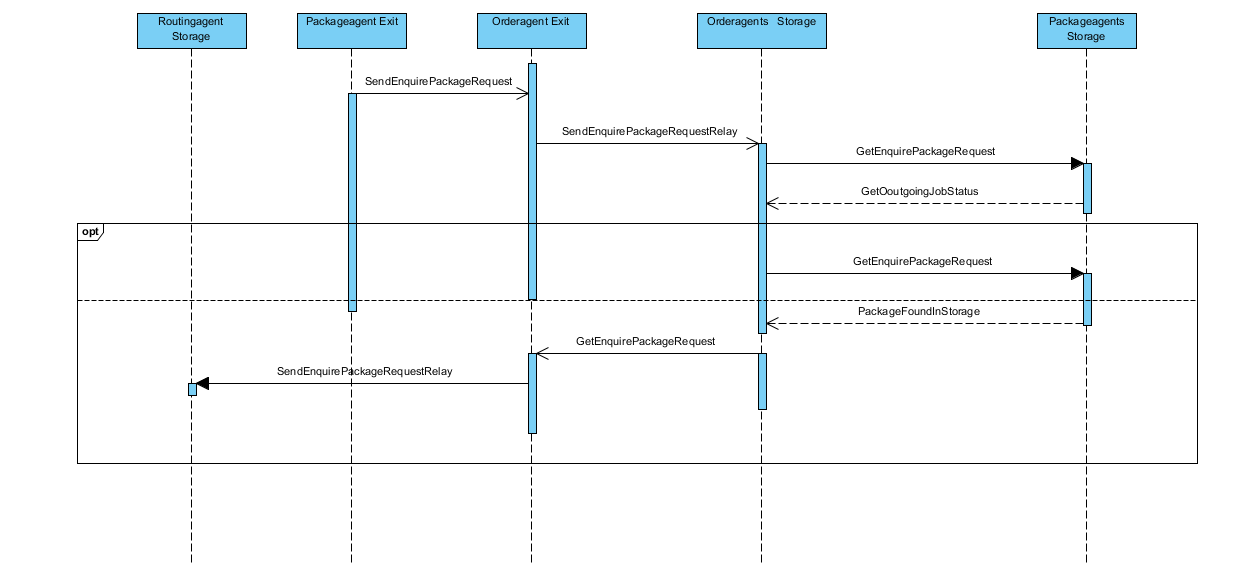
\includegraphics[width=1\textwidth, height=0.6\textwidth]{AusgangZW.png}        
		\caption{Ausgang fragt Zwischenlager}
	\label{Ausgang fragt}
\end{figure}
\newpage
\paragraph{Auktion}
Nachdem ein Paket ein Ziel zugewiesen bekommen hat, startet der Routingagent der jeweiligen Eingangs- oder Zwischenrampe eine Auktion, um ein Fahrzeug zu finden, das das Paket befördert. Abbildung \ref{Auktion} zeigt den Ablauf der Auktion:
\begin{itemize}
\item Der Routingagent schickt eine Nachricht an alle Routingagenten der Fahrzeuge.
\item Die Routingagenten der Fahrzeuge fragen ihre Paketagenten, ob bereits ein Auftrag durchgeführt wird. Der Routingagent wartet bis der Paketagent geantwortet hat.
\item Der Paketagent antwortet dem Routingagenten.
\item Falls das Fahrzeug nicht belegt ist und der Bot auch an keiner anderen Auktion teilnimmt, erfragt der Routingagent seine aktuelle Position von seinem Plattformagenten.
\item Der Plattformagent schickt die aktuelle Position an den Routingagenten.
\item Der Routingagent berechnet mithilfe des Pathfindings eine Aufwandsabschätzung und schickt Sie dem Routingagenten der Rampe. Falls er nicht in der Lage ist, ein Paket zu befördern, teilt er dies der Rampe über die Nachricht mit.
\item Der Routingagent der Rampe speichert alle Estimations nacheinander ab. Haben alle Fahrzeuge geantwortet oder ist der Timeout für die Auktion abgelaufen, wird, sofern vorhanden, der Bot mit der besten Estimation ausgewählt. Falls es einen Bot gibt, der das Paket abholen kann, wird der Paketagent des Zwischenlagers oder Ausgangs benachrichtigt, dass ein Paket in Kürze geliefert wird, damit das IncomingJobFlag gesetzt wird. Dadurch wird verhindert, dass die Bots sich gegenseitig vor einer Rampe blockieren.
\item Der Paketagent antwortet dem Routingagenten nach dem Setzen des Flags.
\item Der Routingagent teilt dem Routingagenten des ausgewählten Fahrzeugs mit, dass es ausgewählt wurde.
\item Der Routinagent des Fahrzeugs sendet eine Nachricht an seinen Paketagenten, um Platz für das Paket zu reservieren.
\item Der Fahrzeug Routingagent leitet die Information an seinen Plattformagenten weiter, damit die Fahrt beginnen kann.
\end{itemize}
\begin{figure}[h!]
	\centering
		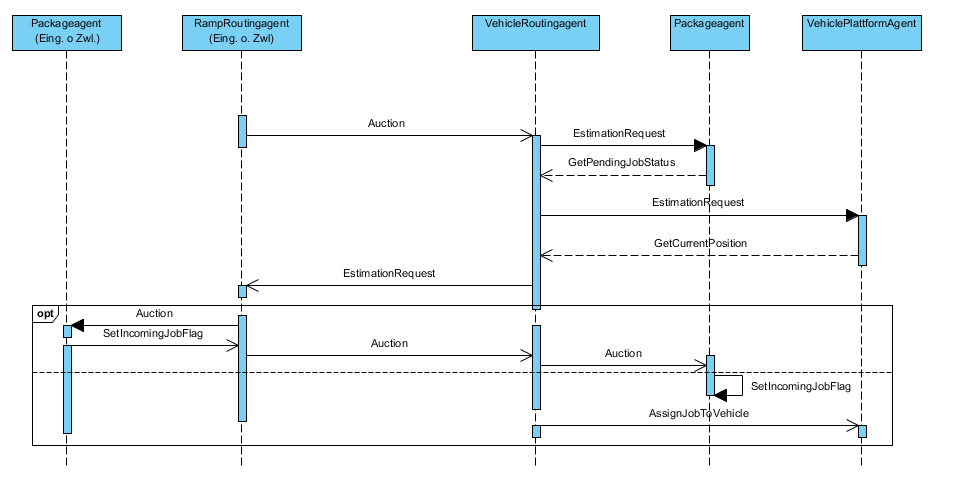
\includegraphics[width=1\textwidth, height=0.6\textwidth]{Auktion.PNG}        
		\caption{Auktion}
	\label{Auktion}
\end{figure}
\paragraph{Paket von Startrampe abholen und zur Zielrampe bringen}
Nachdem das Fahren initiiert wurde, führt der Plattformagent des entsprechenden Fahrzeugs den Transport durch. Abbildung \ref{Fahren} zeigt den Ablauf auf Agentenebene:
\begin{itemize}
\item Das Fahrzeug fährt zur Startrampe und benachrichtigt den Plattformagenten der jeweiligen Rampe.
\item Dieser benachrichtigt seinen Paketagenten, dass das Paket transferiert werden kann. 
\item Der Paketagent sendet eine Nachricht an den Paketagenten des Fahrzeugs, um das Paket zu übergeben und entfernt es von der Rampe.
\item Der Paketagent des Fahrzeugs fügt das Paket hinzu und antwortet dem anderen Paketagenten.
\item Der Paketagent der Startrampe  benachrichtigt den Plattformagenten, dass das Paket übergeben wurde.
\item Dieser benachrichtigt wiederum den Plattformagenten des Fahrzeugs, damit dieser weiß, dass er weiterfahren kann.
\item Der Plattformagent des Fahrzeugs fährt zur Zielrampe und benachrichtigt seinen Paketagenten, dass das Paket übergeben werden kann.
\item Der Paketagent entfernt das Paket und sendet eine Nachricht an den Paketagenten der Rampe, dass das Paket aufgenommen werden soll.
\item Dieser fügt das Paket hinzu und gibt dem Paketagent des Fahrzeugs Bescheid, dass das Aufladen beendet ist.
\item Der Fahrzeug Paketagent informiert seinen Plattformagent, dass der Auftrag erledigt ist.
\end{itemize}
\begin{figure}[h!]
	\centering
		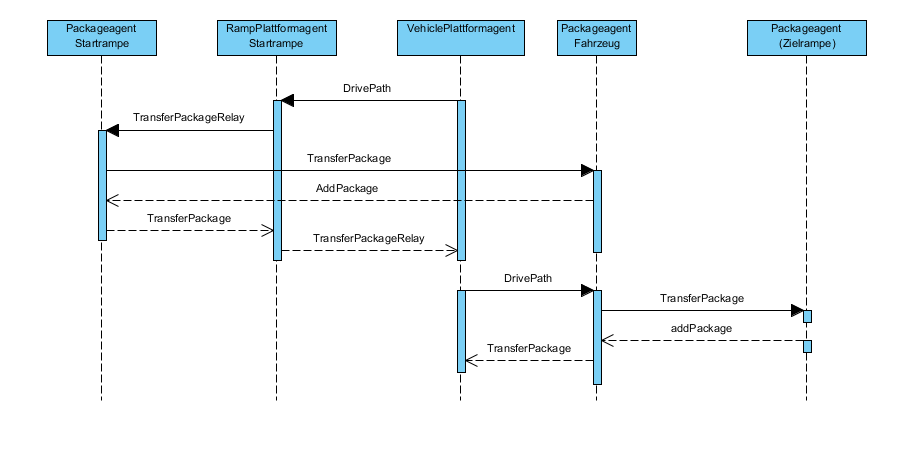
\includegraphics[width=1\textwidth, height=0.6\textwidth]{Fahren.PNG}        
		\caption{Paket abholen und zur Zielrampe bringen}
	\label{Fahren}
\end{figure}
\subsubsection{Implementierung des Pathfindings}
Der entwickelte Pathfindingalgorithmus verwendet eine Karte, die in Kacheln unterteilt ist. Eine Kachel kann dabei entweder als einfache, befahrbare Fläche, als Startposition, als Endposition oder als Hindernis definiert werden. Damit die Simulation um alternative Pathfindingalgorithmen erweitert werden kann, wurde eine einheitliche Schnittstelle definiert, um schnell und einfach (ohne Umbauten von Programmelementen in denen das Pathfinding benutzt wird) mögliche zukünftige Algorithmen einbinden zu können. Diese Schnittstelle ist in Form eines Interfaces definiert. Im Interface sind Funktionen zu finden, die von jeder alternativen Pathfindingroutine implementiert werden müssen. Sollten dabei einige keine Verwendung finden, sollte schlichtweg ein Standardwert zurückgeliefert werden, der sich nicht verändern lässt. Folgende Funktionen sind im Interface vorgesehen:
\begin{itemize}
\item Statusmeldung, ob ein Pfad zur Zeit berechnet wird
\item Anzahl der Zeilen und Spalten in der Liste
\item Position des Start-/Stoppunktes
\item Angabe, ob man diagonales Fahren (de)aktivieren möchte
\item Vermeidung von (möglicherweise unnötigen) Rotationen
\item Initialisierung des Pathfindingalgorithmus
\item Aktuelle Status-(bzw. Fehler-)Meldung
\item Funktion zum Suchen eines Pfades unter andere einer Start- und Stopposition
\end{itemize}

Jede Kachel wird im System als GridItem definiert. Dabei wird in der Kachel die Größe hinterlegt (ist bei allen Kacheln in einer Karte die selbe Größe). Jedes GridItem besitzt einen Typ. Darüber hinaus gibt es noch GridValue und StepValue. GridValue ist dabei der Wert einer Kachel, die bei der Vorwärtssuche ermittelt wurde, wo eine aktuelle Kachel ihre benachbarten freien Kachel einen Wert für die Pfadfindung zugewiesen hat. StepValue repräsentiert hingegen die Anzahl an Schritten im System, um diese Kachel zu erreichen.
\\\\
Damit bei der Rückwärtsberechnung die Punkte eines Pfades gespeichert werden können, wurde die Klasse PathPoint implementiert. Diese kann die Position (x/y-Koortinate) speichern. Sie speichert unter anderem aber auch den Erwartungswert für die Kachel an dieses Position (EstimationValue), welche Aufschluss darüber gibt wie hoch die Kosten (Aufwand) sind um diese Position zu erreichen. Sollte (durch einen zusätzliche Eigenschaft) sich die Richtung der aktuellen Kachel von der vorherigen nicht unterscheiden, hat diese einen kleineren Erwartungswert.
\\\\
Der implementierte Pathfindingalgorithmus wurde hingehen in zwei Klassen implementiert. Bei der einen Klasse handelt sich um eine abstrakte Klasse, welches alle Funktionen, Eigenschaften und Statusmeldungen vom eigentlichen Pathfinding beherbergt, bis auf die Implementation der eigentlichen Pfadsuche. Die Funktion für die Pfadsuche wurde in einer seperaten Klasse implementiert, welche von der abstrakten Klasse erbt (Polymorphie), so dass diese sämliche zu Grunde legende Funktionen verwenden kann. Diese Struktur wurde dahingehend entwickelt, weil der verwendete Suchalgorithmus lediglich einen Pfad ermittelt und zurück liefert. Jedoch wäre es auch möglich den Suchalgorithmus zu modifizieren, um so mehrere alternative Routen auf einer Karte zu ermitteln, die mit bestimmten Kriterien versehen sind. Da diese Suche auch die grundlegenden Funktionen verwenden würde, wurde nur die eigentliche Funktion für die Pfadsuche gekapselt (die Rückwärtsssuche).

\subsubsection{Implementierung der Statistiken}
Nachdem innerhalb des Kapitels \ref{konzept_statistik} das Konzept der Statistiken erarbeitet wurde, geht es in diesem Kapitel darum, die Statistiken umzusetzen. Um Statistiken anbieten zu können, musste zunächst ein geeignetes Framework gefunden werden, mit dessen Hilfe man leich Statistiken erzeugen kann. Hierzu wurde das Framework \textbf{Sencha GXT} gewählt (http://www.sencha.com/products/gxt/). Diese bietet eine Vielzahl von Möglichkeiten, um in einfacher Art und Weise Diagramme zu generieren.

Die Einbindung der Diagramme erfolgt über Popups. So hat der Benutzer die Möglichkeit, nach belieben die für ihn interessante Statistik ein- bzw. auszublenden. 

Die Berechnung der Statistiken erfolgt mithilfe des Statistik-Agenten, der eigens dafür in die Simulation eingebracht wird. Dieser wird an definierten Stellen von den unterschiedlichen Agenten aufgerufen, wenn ein bestimmtes Ereignis eingetreten ist (z.B. Ein Auftrag verlässt die Simulation, ein Bot wechselt seinen Status von Arbeitend auf Wartend, ...). Diese Daten werden dann vom Statistik-Agenten aufgefangen und zu seiner Datenhaltung hinzugefügt. Sobald ein Ereignis eine Neuberechnung einer Statistik erfordert, informiert der Statistik-Agent die UI und fordert eine Neuzeichnung dieser. So erhält der Benutzer sofort Feedback über das soeben eingetretene Ereignis. Die Kommunikation zwischen Server und Client erfolgt hier mithilfe von AJAX. Die Ergebnisse werden dem Benutzer also nahezu Live präsentiert. 

Die Statistiken sind in der Simulation im Reiter "Statistiken" zu finden.

\subsubsection{Interaktion der Komponenten}
In Abschnitt \ref{Interaktion der Komponenten} wurden die Interaktionen der Systemkomponenten auf logischer Ebene beschrieben, die für das Starten einer Simulation bis hin zur Visualisierung notwendig sind. Im Folgenden Abschnitt soll beschrieben werden, wie und mit welchen Mitteln die einzelnen Schritte implementiert wurden. 
\paragraph{Client-Server Kommunikation}
Das Starten einer Simulation wird über das Menuitem \glqq Starten/Anhalten\grqq ausgelöst (s. Abbildung\ref{RPCS}). Wird das Menuitem gedrückt, dann wird die Methode execute ausgeführt. In der Methode wird geprüft, ob die Simulation bereits läuft, um festzustellen, ob die Simulation gestartet oder angehalten werden soll. Wenn die Simulation noch nicht gestartet wurde, wird zunächst geprüft, ob das erstellte Szenario konsistent ist (Mindestens eine Eingangs- und Ausgangsrampe). Wenn dies der Fall ist, wird die Simulation gestartet. Dies erfordert eine Client-Server Kommunikation. Die Implementierung erfolgt durch den von GWT bereitgestellten Remote Procedure Call (RPC) Mechanismus (Vgl. \cite{gwtrpc}). 
\\\\
Die  Variable agentPlatformService referenziert das Interface AgentPlatformServiceAsync. Serverseitig gibt es ein Servlet \glqq AgentPlatformService\grqq , das verschiedene Methoden bereitstellt, die über das Interface AgentPlatformServiceAsync aufgerufen werden können. Die Variable ist als AgentPlatformServiceAsync Interface deklariert, wird aber mit einer automatisch generierten Proxy-Klasse instantiiert (s. Quellcode/Konstruktor der Klasse MainframePresenter). In der Methode execute wird über den Aufruf der Methode startSimulation das Szenario übergeben und zum Server geschickt. Für den Aufruf ist ein Objekt notwendig, das das Interface AsyncCalback implementiert, welches wiederum der Methode als interne Klasse übergeben wird. Der Typparameter, in diesem Fall ein Integer, definiert, welcher Rückgabewert vom Server erwartet wird. Außerdem wird in den Methoden onFailure und onSuccess definiert, was passieren soll, wenn der RPC fehlschlägt bzw. erfolgreich war. Wenn die Simulation serverseitig erfolgreich gestartet wurde, dann soll die auf dem Server generierte ID dem aktuellen Szenario zugewiesen werden und der Status der Simulation auf gestartet gesetzt werden.    
\begin{figure}[h!]
	\centering
		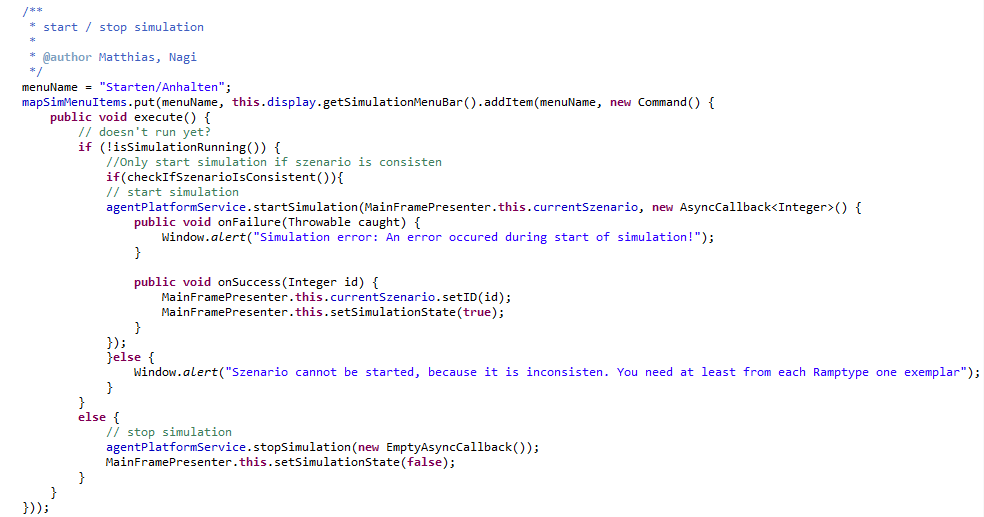
\includegraphics[width=1\textwidth, height=0.6\textwidth]{RPCS.PNG}        
		\caption{Starten einer Simulation}
	\label{RPCS}
\end{figure}
\paragraph{Start des Multiagenten-Systems}
Nachdem die Daten zum Server geschickt wurden, wird die Methode startSimulation des Servlets AgentPlatformServiceImpl aufgerufen. Für das Szenario wird eine ID generiert und über das Object Array wird das Szenario allen Agenten als Parameter zur Verfügung gestellt. Danach wird eine Agentenplattform für das jeweilige Szenario gestartet. Die Liste der Conveyor (Fahrzeuge und Rampen) aus dem Szenario wird durchlaufen und für jeden Conveyor werden die benötigten Agenten erzeugt. Die Methode addAgentToSimulation erzeugt anhand der Conveyor- und Szenario-ID einen eindeutigen Namen für jeden Agenten, übergibt die Parameter und fügt ihn der Simulation hinzu. Anschließend wird der Jobagent initialisiert und die Agenten werden gestartet. Die letzte Anweisung schickt die Szenario ID zum Client zurück.
\\\\  
\begin{figure}[h!]
	\centering
		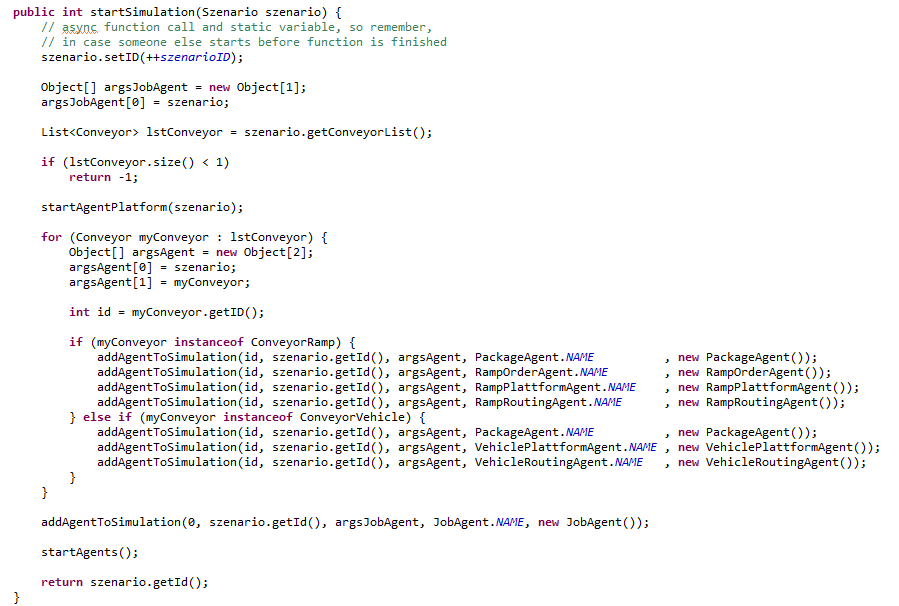
\includegraphics[width=1\textwidth, height=0.6\textwidth]{StartMAS.PNG}        
		\caption{Starten des MAS}
	\label{SMAS}
\end{figure}
\\\\
\paragraph{Start des Jobtimers} 
Nachdem der Jobagent alle Informationen erhalten hat, die er für die Zuweisung von Aufträgen benötigt, schickt er eine Nachricht an den Client, dass die Aufträge zum Server geschickt werden können (Vgl.Abschnitt \ref{Jobagent}). Der Client startet den Jobtimer mit der Methode startJobTimer des MainframePresenters (s.Abbildung \ref{jobtim}). Die Integer Variable elapsedTimeSec repräsentiert die Zeit. Der Timer wird gestartet und die run-Methode wird kontinuierlich ausgeführt, bis der Jobtimer gestoppt wird. Die Zeitvariable wird bei jedem Durchlauf um eins hochgezählt, was bedeutet, dass eine Sekunde vergangen ist. Die einzelnen Jobs aus der Liste werden in der for-Schleife abgefragt und ihr Zeitstempel wird mit der elapsedTimeSec Variable abgeglichen. Ist die vergangene Zeit größer oder gleich der Zeit zu der ein Job ausgeführt werden soll, dann wird der Job mit der Methode addJob zum Server geschickt. Mit der vorletzten Anweisung wird festgelegt, in welchen Zeitabständen der Timer ausgeführt werden soll. Die letzte Anweisung dient dazu, den Timer initial zu starten.
\\\\
\begin{figure}[h!]
	\centering
		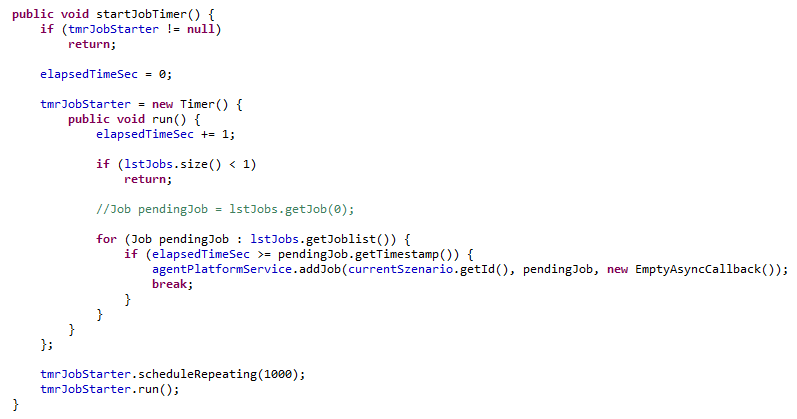
\includegraphics[width=1\textwidth, height=0.6\textwidth]{Jobtimer.PNG}        
		\caption{Start des Jobtimers}
	\label{jobtim}
\end{figure}
\\\\
Abbildung \ref{jobtimserv} zeigt die serverseitige Weiterleitung des empfangenen Auftrags. In der Methode addJob des AgentPlatformServiceImpl Servlets wird der jeweilige Jobagent anhand der Szenario ID aus einer Hashmap geholt. Es wird ein ACLMessageObjekt erzeugt und der Nachrichtentyp wird im Konstruktor festgelegt, um gezielt die notwendige Behaviour zu adressieren. Als Empfänger wird der Jobagent selber festgelegt. Anschließend wird der Job der Nachricht als ContentObject hinzugefügt und versendet.
\\\\
\begin{figure}[h!]
	\centering
		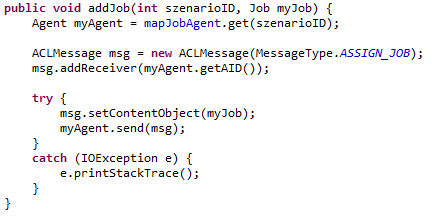
\includegraphics[width=0.8\textwidth, height=0.4\textwidth]{addJob.PNG}        
		\caption{Weiterleitung des Auftrags}
	\label{jobtimserv}
\end{figure}
\newpage
\paragraph{Visualisierung von Zustandsveränderungen}
Die einzelnen Agenten führen Aktionen durch. Werden dadurch Zustände verändert (z.~B. Hinzufügen eines Pakets etc.), müssen diese visualisiert werden. Das MAS läuft auf dem Server. Damit ein Client die Zustandsveränderungen visualisieren kann, muss er vom Server über die Art der Zustandsveränderung informiert werden. Das Schicken von Nachrichten vom Server zum Client wurde mithilfe des GWT Eventservices implementiert. Der Eventservice ist ein event-basiertes Kommunikationsframework, dass auf dem GWT-RPC Mechanismus und der Comet Server-Push Technologie basiert (Vgl. \cite{gwteventservice}). Abbildung \ref{addEvent} zeigt die Methode AddPackage des Packageagents, die für das Hinzufügen eines Pakets benötigt wird. Nachdem das Paket in die Liste eingefügt wurde, wird mithilfe der Klasse EventHelper ein Event zum Client gefeuert. Der EventHelper erbt von dem Servlet RemoteEventServiceServlet, das vom EventService Framework bereitgestellt wird und das GWT-Servlet, um die Funktionalität zum Versenden von Events erweitert (Vgl.\cite{gwteventservice}). 
\\\\
\begin{figure}[h!]
	\centering
		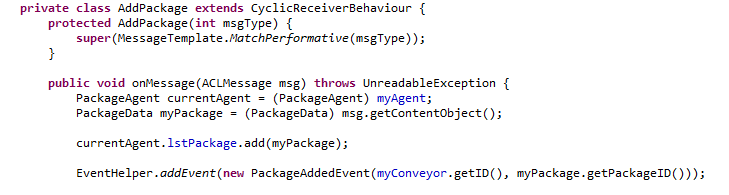
\includegraphics[width=0.8\textwidth, height=0.4\textwidth]{addEvent.PNG}        
		\caption{Feuern eines Events}
	\label{addEvent}
\end{figure}
\\\\
Die Klasse PackageAddedEvent ist eine selbst definierte Event-Klasse, die das Interface Event des Eventservices implementiert (Vgl.\cite{gwteventservice}). Mithilfe dieser Klasse können Informationen für den Client transportiert werden. Die Informationen werden im Konstruktor der Klasse PackageAddedEvent übergeben. In diesem Fall werden die Conveyor- und Package-ID übergeben, damit der Client weiß, welchen Conveyor er neu zeichnen soll und welches Paket mit welcher ID hinzugefügt wurde.
\\\\
Abbildung \ref{addEventClient} zeigt die clientseitige Verarbeitung der Events, die vom Server empfangen werden. In der Methode HandleEvents des Mainframepresenters , wird zunächst eine Instanz der Klasse RemoteEventService über die RemoteEventServiceFactory geliefert. Alle vorhandenen Listener werden entfernt und es wird ein neuer Listener hinzugefügt. Beim Hinzufügen des Listeners wird eine Domain mit einer Zeichenkette übergeben. Durch die Domain kann gezielt festgelegt werden, für wen eine Nachricht bestimmt ist (Vgl.\cite{gwteventservice}). Die Zuordnung einer Nachricht zu einer Domain, wird beim Versenden der Nachricht festgelegt (S. Quellcode Klasse EventHelper). In der Methode apply des Listeners wird für alle definierten Events festgelegt, welche Aktion beim Empfang auf dem Client ausgeführt werden soll. Beispielsweise wird durch das SimStartedEvent das Starten des Jobtimers durch die Methode startJobTimer initialisiert.
\\\\  
\begin{figure}[h!]
	\centering
		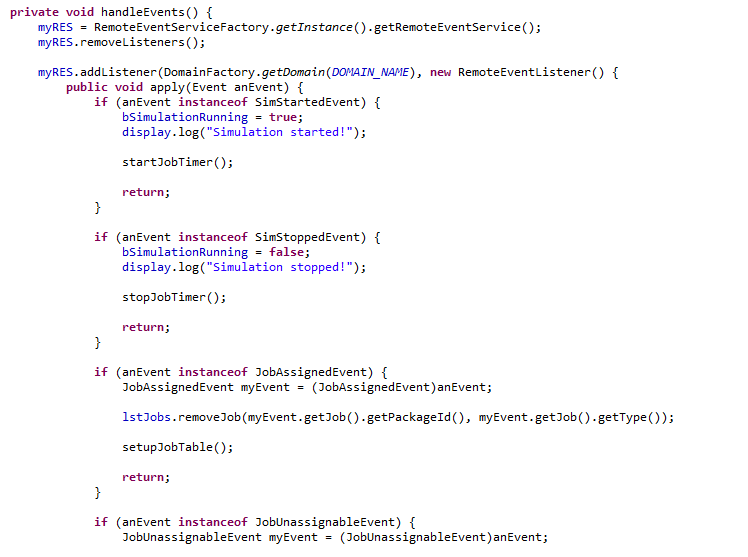
\includegraphics[width=1\textwidth, height=0.6\textwidth]{Vis.PNG}        
		\caption{Clientseitige Verarbeitung des Events}
	\label{addEventClient}
\end{figure} 
\newpage
\subsection{Testen und Validieren}
Das Artefakt, welches zuletzt ausgebracht werden soll, wird mithilfe verschiedener Werkzeuge validiert. Dazu gehören mitunter Unit-Tests und manuelle UI-Tests. Mithilfe der Unit-Tests werden verschiedene Komponenten innerhalb der Software getestet und dessen Funktionsweise mithilfe dessen garantiert. Unit-Tests sind aber nur dann ein probates Mittel, wenn man abgeschlossene Funktionen innerhalb der Software testen möchte. Sobald es darum geht, Anordnung und Funktionsweise von UI-Komponenten zu testen (wie z.B. die Bewegung der Bots), reichen die Möglichkeiten von Unit-Tests leider nicht mehr aus. Zu diesem Zwecke könnte man automatisierte UI-Tests implementieren. Diese sind aber nur schwer zu realisieren und bedürfen einem hohen Arbeitsaufwand bei der initialen Realisierung. Zunächst müsste die Infrastruktur für solche Tests bereitsgestellt werden und in der Praxis hat sich gezeigt, dass diese einen sehr hohen Wartungsaufwand benötigen. Aus diesem Grund wurde hier auf automatisierte UI-Tests verzichtet und wurden durch manuelle Tests ersetzt. Nachdem die Simulationsmitglieder Features ausgebracht haben, wurden jeweils eine handvoll UI-Tests durchgeführt, die die Korrektheit UI versichert haben. Zu diesem Testset gehören folgende Tests mit den jeweiligen Akzeptanzkriterien:

\begin{itemize}
\item Laden eines Szenarios.
	\begin{itemize}
	\item Sind die Objekte korrekt auf der UI angeordnet und charakterisiert (wird der Bot als Bot erkannt oder fälschlicherweise als Rampe / Wand)?
	\end{itemize}	
	
\item Aktuere können per Drag and Drop in dem Szenario anders platziert werden
	\begin{itemize}
	\item Die Aktuere lassen sich mit der linken Maustaste aufheben
	\item Ein Aktuere der soeben aufgehoben wurde, kann durch erneutes linksklicken, neu platziert werden
	\end{itemize}	

\item Speichern eines geänderten Szenarios.
	\begin{itemize}
	\item Das Szenario wird nach dem speichern korrekt, mit den vorgenommenen Änderungen geöffnet.
	\item Das alte Szenario wurde nicht überschrieben
	\end{itemize}	
	
\item Ausführen der Simulation
	\begin{itemize}
	\item Die Simulation läuft über 5 Minuten stabil
	\item Es wird keine Exception im in der Logausgabe erzeugt
	\item Die UI wird über Bewegungen der Aktuere informiert und zeichnet diese wie erwartet
	\end{itemize}	

\end{itemize}
	

	% Chapter 6 Komponentenbeschreibung
	\clearpage
	\ohead[Komponentenbeschreibung]{Komponentenbeschreibung}
	\chead[Uni Oldenburg]{Uni Oldenburg}
	\ihead[PG FAISE]{PG FAISE}
	\setheadtopline{1pt}
	\setheadsepline{0.5pt}
	\ofoot[Endbericht]{Endbericht}
	\cfoot[\pagemark]{\pagemark}
	\ifoot[30. September 2014]{30. September 2014}
	\setfootsepline{0.5pt}
	\setfootbotline{1pt}
	\section{Teilbericht Materialfluss}
Das Ziel der Materialflussgruppe ist das dezentrale Management der Fördereinheiten auf den Rampen und auf dem Volksbots.

\subsection{Anforderungen}
In diesem Abschnitt werden die gestellten Anforderungen zusammengetragen. Wir unterscheiden dabei zwischen funktionalen Anforderungen, die die direkte Funktionalität des fertigen Systems beschreiben, und nicht-funktionalen Anforderungen, die die qualitativen Eigenschaften des Systems widerspiegeln.
\subsubsection{Funktionale Anforderungen}
\begin{enumerate}
\item \textbf{Plattform}: Die physische Zelle wird als Netzwerk von Knoten in einem drahtlosen Sensornetzwerk implementiert. Als Plattform dienen MICAz-Module mit Atmel ATMega 128 Mikrocontroller und CC2420 Funkchip (siehe \autoref{MICAZ}).
 \item \textbf{Aktorik/Sensorik}: Die Rampen verfügen über Magnetstifte zum Vereinzeln der Pakete und Lichtschranken zum Erkennen von Paketen. Sie werden von den MICAz-Modulen angesteuert beziehungsweise ausgelesen.
 \item \textbf{Kommunikation}: Die MICAz-Module auf Rampen und Volksbots kommunizieren drahtlos untereinander auf Basis von Agenten-Nachrichten.
 \item \textbf{Synchronisation}: Die Simulation wird über ein Micaz-Modul, das als Gateway fungiert, an die drahtlose Kommunikation angebunden. Die Synchronisation der Zustände erfolgt über eine serielle Schnittstelle.
 \item \textbf{Disposition}: Die Controller kennen den Belegungszustand der Rampe und generieren nach dem FIFO-Prinzip Aufträge, die sie an die Volksbots vergeben.
 \item \textbf{Übergabe}: Wenn eine Ein- oder Auslagerung an einer Rampe ausgeführt werden soll, so übernimmt der Controller der Rampe die Kontrolle über die Fördereinheit des Fahrzeugs und sorgt dafür, dass das Paket verladen wird.
 \item \textbf{Kooperation}: Einsatz kooperativer Lösungsstrategien für die Materialflusssteuerung, Überwachung und Steuerung mittels Multi-Agentensystem.
\end{enumerate}

\subsubsection{Nicht-funktionale Anforderungen}
\begin{enumerate}
\item \textbf{Ressourcen}: Bei der Entwicklung muss 
auf den sparsamen Umgang mit Hardwareressourcen (Rechenzeit, Kommunikationsbandbreite, Speicher) geachtet werden. Insbesondere der vorhandene Arbeitsspeicher und das Kommunikationsmedium dürfen nicht überlastet werden, um einen stabilen Betrieb zu garantieren. 
\item \textbf{Stabilität}: Es müssen Maßnahmen getroffen werden, um ein stabiles System zu schaffen. Dies gilt insbesondere für die möglichst verlustfreie Übertragung von drahtlosen Nachrichten.
\item \textbf{Volksbots}: Die Module des Materialfluss über eine definierte Schnittstelle mit den Fahrzeugen kommunizieren, um auf die Aktorik und Sensorik der Volksbots zugreifen und schließlich einen Transport der Pakete gewährleisten zu können.
\end{enumerate}

\subsection{Beschreibung der Komponenten}
Dieser Abschnitt beschreibt die physikalischen Komponenten, die von der Teilgruppe Materialfluss verwendet wurden. Zu den diesen Komponenten zählen die Rampen, sowie die \textsc{Mica}z-Module mit ihren Mikrocontrollern. 
\subsubsection{Rampen}
Rampen stellen Ein- und Ausgänge, sowie Zwischenlager im physischen System dar. Auf einer Rampe finden bis zu vier Pakete Platz. Bolzen hinter dem ersten Paket, separiert dieses von den anderen Dreien. Damit das vorderste Paket nicht vorne von der Rampe herunterfällt, sind an der Vorderseite zwei weitere Bolzen angebracht. 

Durch vier Lichtschranken, wird eine Überwachung der Rampe ermöglicht. Diese beinhaltet zum einen das Abfragen, wie viele Pakete auf einer Rampe liegen. Zum anderen kann durch die Überwachung überprüft werden, an welcher Stelle Pakete liegen.

Alle vier Bolzen sind seitlich der Rampe befestigt. Eine autonome Steuerung der Rampen, wird durch ein angebrachtes \textsc{Mica}z-Modul ermöglicht.
\autoref{fig:skiram} zeigt ein Beispiel solch einer Rampe.

\begin{figure}[h!]
	\centering
		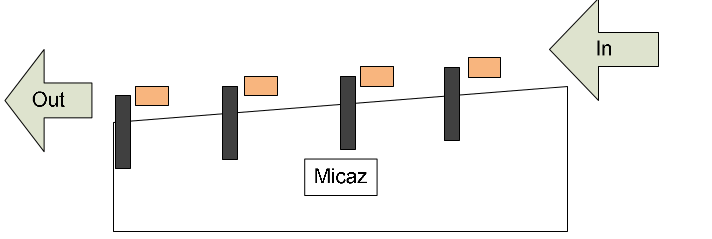
\includegraphics[width=0.9\textwidth]{SkizzeRampe.png}
	\caption{Beispiel einer eingesetzten Rampe}
	\label{fig:skiram}
\end{figure}

\subsubsection{Mikrocontroller}
Ein Mikrocontroller ist ein vollständiger Kleinstrechner auf einem einzigen Chip, dessen Zentraleinheit aus einem oder mehreren Mikroprozessen besteht. Zusätzlich enthält ein Mikrocontroller Speicher und Ein- bzw. Ausgabeschnittstellen zur Außenwelt. Dazu können neben einfach Ausgangspins auch komplexere Busprotokolle wie etwa USART, SPI oder CAN gehören.

Mikrocontroller werden eingesetzt, wenn eine Kommunikations- oder Steuerungsaufgabe mit möglichst geringen Ressourcen (Baugröße, Energie, Kosten) gelöst werden müssen. Die in einem Mikrocontroller verbauten Prozessorkern, Speicher und die Aus- und Eingabeschnittstellen, sind auf die Lösung derartiger Aufgaben zugeschnitten. Die große Anzahl an potenziellen Aufgabenstellungen hat zur Folge, dass es eine Vielfalt von Mikrocontrollern gibt. Meist sind die Mikrocontroller deshalb in Mikrocontrollerfamilien aufgeteilt. Innerhalb einer Familie unterscheiden sich die Controller nicht im Prozessorkern, sondern im verfügbaren Speicher und in den Ein- und Ausgabeschnittstellen \cite{ECHT2005}. In \autoref{fig:aufbmc} ist der schematische Aufbau eines MCs dargestellt.
\begin{figure}[th]
	\centering
		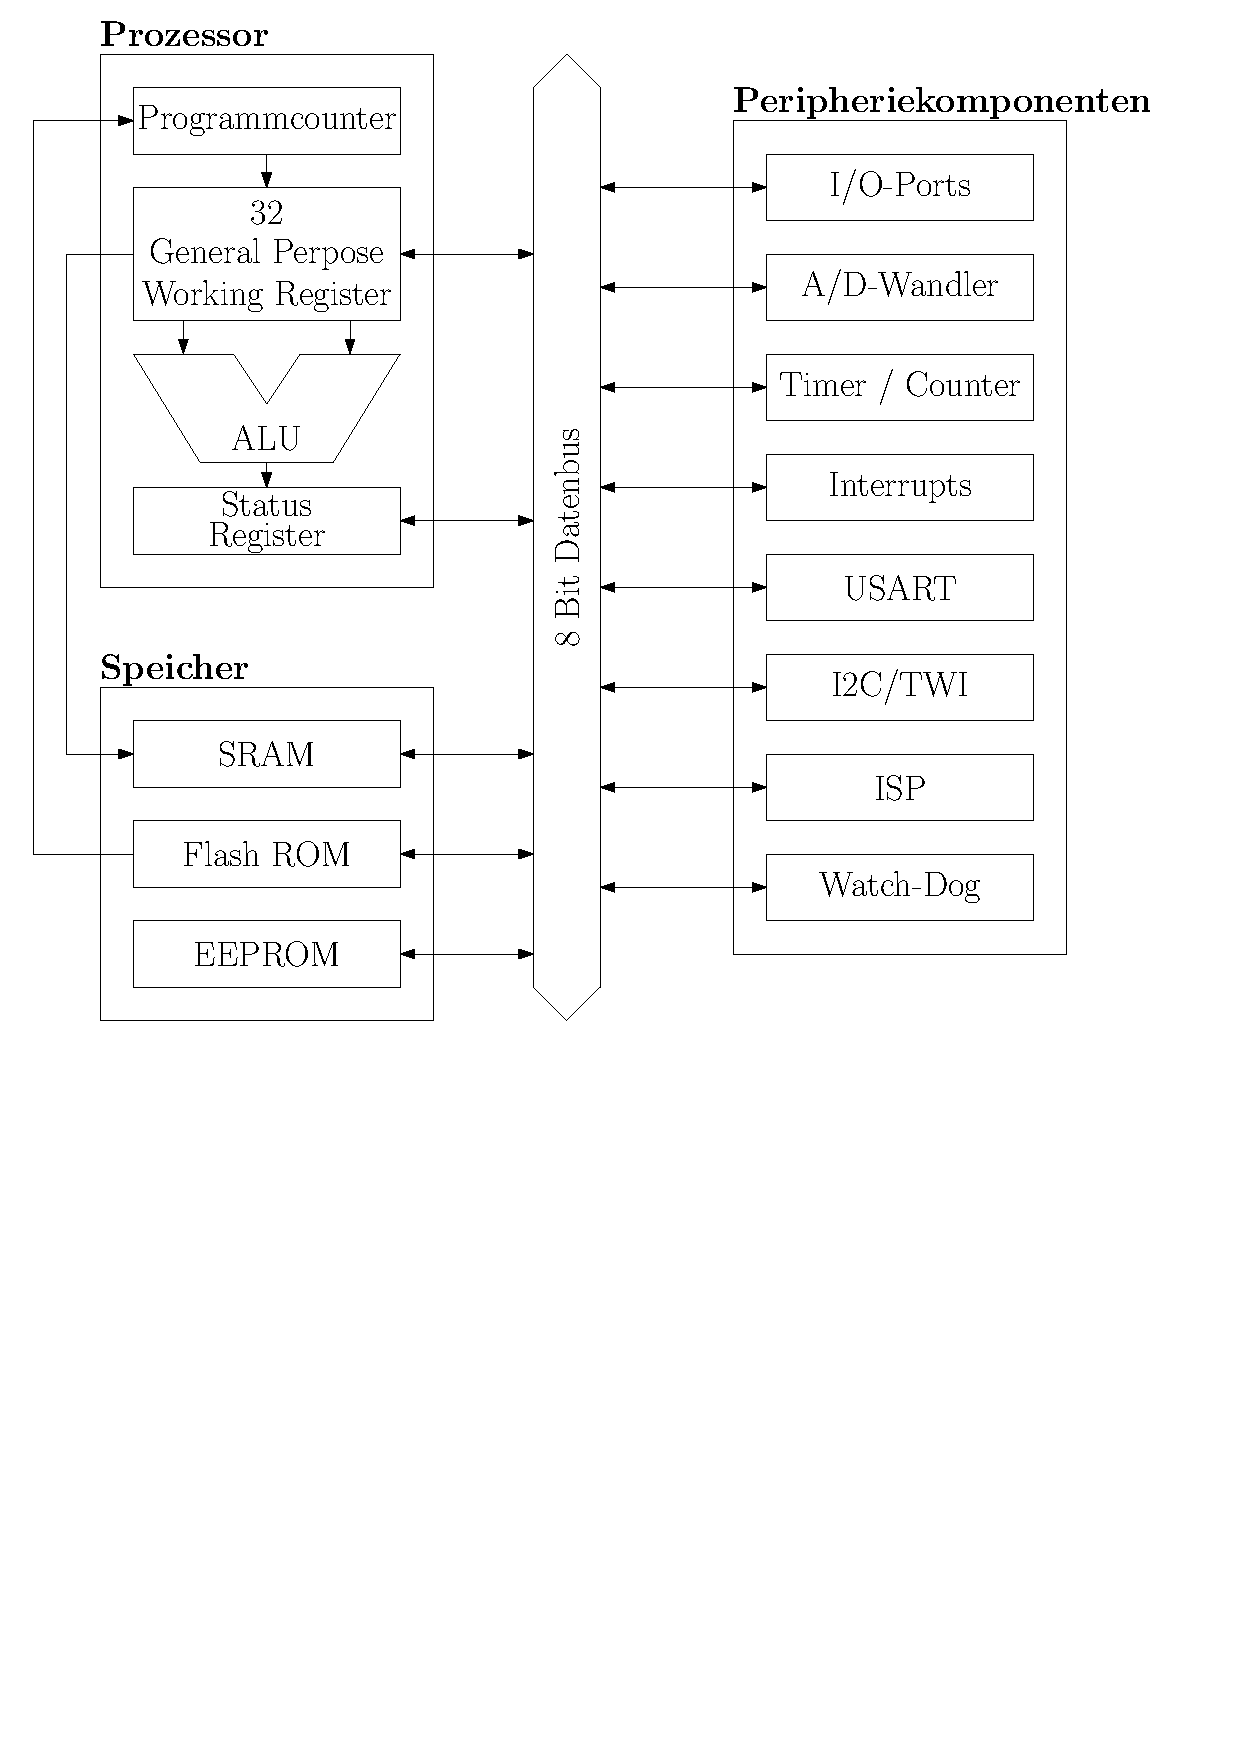
\includegraphics[width=0.8\textwidth]{flow/schemamc.pdf}
	\caption{Schematischer Aufbau eines Mikrocontrollers vgl. \cite{Brinkschulte:2002:Mikrocontroller}}
	\label{fig:aufbmc}
\end{figure}

Die zentrale Steuereinheit eines MCs ist der \textbf{Prozessor} (engl.: Central Processing Unit (CPU)). Sie ist die wichtigste Funktionseinheit und für die Verarbeitung von Befehlen und arithmetischen Berechnungen verantwortlich. Über den internen Bus kann die CPU mit weiteren Grundbausteien kommunizieren und beispielsweise auf Daten innerhalb des Speichers zugreifen.

Der \textbf{Speicher} besteht in der Regel aus dem Arbeitsspeicher (RAM, kurz für: Random Access Memory) und dem Programmspeicher bzw. Flash-Speicher. Normalerweise werden diese zwei Speichertypen logisch voneinander getrennt. Programme werden im nichtflüchtigen Flash-Speicher gesichert. Dieser kann mehrere Kilobyte (KB) bis Megabyte (MB) umfassen. Bei speziellen Systemen ist es möglich den Programmspeicher durch externe Flash-Komponenten zu erweitern um zusätzlichen Speicherplatz zu gewinnen.

Zwischenergebnisse, Messwerte von Sensoren, Steuergrößen usw. werden auf dem RAM abgelegt. Dieser ist deutlich schneller als der Flash-Speicher, verfügt aber in der Regel über deutlich weniger Speicherplatz. Alle Werte, welche zur Laufzeit im RAM abgelegt werden, sind im Gegensatz zum Flash-Speicher flüchtig. Das bedeutet, dass Daten bei einem Neustart des Mikrocontrollers nicht erhalten bleiben.

Durch die \textbf{Peripheriekomponenten} wird die Verbindung und Kommunikation zwischen Controller und Außenwelt ermöglicht. Über die digitalen Ein- und Ausgänge (GPIO, kurz für: General Purpose Input/Output) können Sensoren, Aktoren oder andere Systeme mit dem Mikrocontroller verbunden werden. Die meisten Mikrocontroller bieten eine Vielzahl von Ein- und Ausgängen \cite[S. 13-16]{SOM2012}.

Bei der Umsetzung des Projekts wurden \textsc{Mica}z-Module eingesetzt. Im Folgenden werden kurz die Eigenheiten dieser Module erläutert.

\paragraph{\textsc{Mica}z-Modul}
Ein \textsc{Mica}z-Modul ist drahtloser Sensornetzwerkknoten von der Firma Memsic. Mehrere dieser Module übernehmen in der physischen Zelle die Berechnung Geschäftslogik und die Steuerung der Rampen. \autoref{fig:micaz} zeigt ein solches Modul, während \autoref{fig:blockmicaz}  ein Blockdiagramm von dessen Struktur darstellt. Herzstück der Module ist ein ATMega128L-Mikrocontroller. Bei diesem handelt es sich um einen Low-Power-Mikrocontroller von der Firma Atmel. Darüber hinaus verfügt ein \textsc{Mica}z-Module über einen CC2420-Funkchip der Firma Texas Instruments. Dieser ermöglicht die drahtlose Kommunikation mit anderen Modulen auf einer Frequenz von 2.4 GHz ermöglicht. Es wird dabei der IEEE 802.15.4 Standard verwendet. Eine Antenne kann über eine MMCX-Schnittstelle mit dem Modul verbunden werden, um Signalstärke und -reichweite zu erhöhen. Weiter verfügen die Module über einen 128 KB großen Flash-Speicher.
Zugang zu einee Vielzahl der Leitungen des Moduls gewährt ein 51-poliger Steckverbinder. Über eine Erweiterungsplatine werden so etwa die Lichtschranken und Magnetbolzen der Rampe angeschlossen. Denkbar wäre auch ein größerer Arbeitsspeicher, alle nötigen Pins des Mikrocontrollers sind über den Steckverbinder erreichbar.
Im Projekt wurde die Steckverbindung weiterhin dafür genutzt, die \textsc{Mica}z-Module über ein \textsc{Mib}520 an einen PC anzuschließen, um sie über eine UART-Schnittstelle auszulesen und per JTAG (siehe \autoref{sec:JTAGICE3}) zu programmieren \cite{MICSHEET,C2420SHEET}.

\begin{figure}[th]
  \centering
    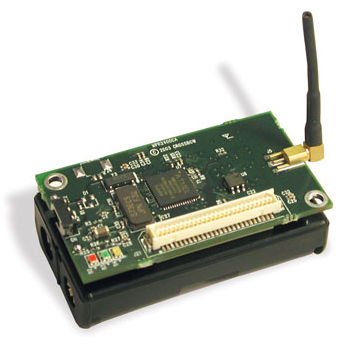
\includegraphics[width = 0.4\textwidth]{flow/micaz.png}
    \caption{\textsc{Mica}z-Modul \cite{Memsic:2014:Online}}
    \label{fig:micaz}
\end{figure}

\begin{figure}[th]
  \centering
    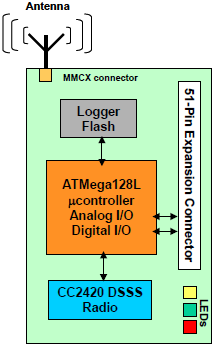
\includegraphics[width = 0.4\textwidth]{flow/blockmicaz.PNG}
    \caption{Blockdiagramm der \textsc{Mica}z-Module  \cite{Memsic:2014:Online}}
    \label{fig:blockmicaz}
\end{figure}

\paragraph{\textsc{Mib}520}
Ein \textsc{Mib}520 stellt eine Schnittstelle für \textsc{Mica}z-Module dar. Es erlaubt die Verbindung eines \textsc{Mica}z-Moduls mit einem Computer per USB-Schnittstelle. So kann über die USART-Schnittstelle des Moduls mit dem PC kommuniziert werden. Über diese Verbindung wurde die Schnittstelle zu den Volksbots realisiert. Weiterhin verfügt ein \textsc{Mib}520-Gateway über eine \textbf{JTAG}-Schnittstelle.


\subsection{Werkzeuge}

\subsubsection{Robot Operating System (ROS)}

Es gibt viele Robotik-Frameworks, die spezifisch für präzise Anwendungen, für Prototypen,
erstellt wurden. ROS strebt da eher das Allgemeine an. Das »Robot Operating System«
(ROS) ist ein Open-Source Framework für individuelle Roboter, das sich in der
Robotikforschung in den letzten Jahren etabliert hat und ein großes Repertoire an Software-Komponenten und -Werkzeugen für Robotikapplikationen bietet.\\
Die Entwicklung begann 2007 am Stanford Artificial Intelligence Laboratory im Rahmen des
Stanford-AI-Robot-Projektes (STAIR). Heute wird es hauptsächlich am Robotik Institut Willow
Garage weiterentwickelt. Seit April 2012 wird ROS von der neu gegründeten,
gemeinnützigen Organisation Open Source Robotics Foundation (OSRF) unterstützt. Die
Bibliotheken von ROS setzen auf Betriebssysteme wie Linux, Mac OS X oder Windows auf.
ROS ist nicht von einer spezifischen Sprache abhängig. Heutzutage gibt es 3 Grundlibraries
für ROS, die jeweils auf Python, Lisp und C++ ausgerichtet sind. Zwei Exmperimentier-
Librairies sind für Java und Lua erhältlich.
\subsubsection*{Was will ROS?}
\begin{itemize}
 \item ROS will unterstützen, Code für Forschung und Entwicklung wiederzuverwenden
 \item loser Verbund von individuellen Programmteilen (Nodes)
 \item einzelne Programmteile können einfach geteilt und verbreitet werden (Packages und Stacks)
 \item ROS stellt Repositories zu Verfügung, um dort Code zu teilen \cite{ROS:2014:Online}
(http://www.ros.org/browse)
\end{itemize}
\subsubsection*{Was kann ROS?}
Die Hauptbestandteile und Hauptaufgaben von ROS sind Hardwareabstraktion; Gerätetreiber; Implementierung 
von viel genutzten Funktionalitäten; Inter-Prozess-Kommunikation; Paket-Management
\subsubsection*{Aufgaben des ROS}
\begin{itemize}
 \item Interprozesskommunikation (IPC)
 \begin{itemize}
\item Problematik der Kommunikation zwischen verschiedenen Systemen des Roboters
\item Sicherheitseinstellung bei der Übertragung
\item Anforderung an die Geschwindigkeit / Schnelligkeit der Kommunikation
\item Koordination von Nachrichten durch zentralen Master
\end{itemize}
\item Paketverwaltung – Packages
\begin{itemize}
 \item ROS ist durch Softwarepakete (sogn. Packages) aufgebaut
 \item Ein Package beinhaltet Laufzeitprozesse (Nodes); ROS abhängige Bibliotheken;
Datensätze; Konfigurationsdateien;3rd Party Software
 \item Packages sind dazu, da um Code wiederverwendbar zu machen
\end{itemize}
\item Paketverwaltung – Stacks
\begin{itemize}
\item Sammlung von Paketen (Packages)
\item Der Sinn ist, dass Stacks die Verteilung und Verwendbarkeit von Code
vereinfachen
\item Meist viele Packages ähnlicher Aufgaben in einem Stack verpackt
\end{itemize}
\item Message (msg)
\begin{itemize}
 \item  Messages werden verwendet um unter ROS Nachrichten zwischen Knoten und
Topics auszutuaschen
\item Dafür verwendet ROS eine einfache Beschreibung der Datentypen in Textdateien
\item Durch diese Beschreibung kann für unterschiedliche Sprachen Code autogeneriert
werden
\item Diese sind in .msg-Dateien im msg- Unterverzeichnis eines ROS-Pakets abgelegt
\item Eigene Message-Typen sind mit Paket Ressource-Namen bezeichnet
\item Standard Messages sind mit std\_msg/msg/String.msg bezeichnet
\end{itemize}
\item Service
\begin{itemize}
 \item ROS verwendet eine eigene vereinfachte Service Description Language ("srv") für die
Beschreibung von ROS Service-Typen
\item Setzt direkt auf die ROS msg-Format auf
\item Ermöglicht die Anfrage / Antwort-Kommunikation zwischen den Knoten
\item Service-Beschreibungen sind in .srv-Dateien im srv- Unterverzeichnis eines Pakets
gespeichert
\item Service-Beschreibungen werden für die Verwendung mit dem Paket Ressource-
Namen bezeichnet
\item Z. B.: wird die Datei robot\_srvs/srv/SetJointCmd.srv als Service
robot\_srvs/SetJointCmd bezeichnet
\end{itemize}
\item Notes
\begin{itemize}
 \item Der Nachrichtenaustausch findet bei Nodes durch 3 Möglichkeiten statt: Parameter
Server;Topics; Services
\item Nodes werden wie in einem Graph angeordnet
\item In einem System laufen viele Nodes Parallel
\item Diese werden zu Beginn gestartet
\item Beispiele sind Nodes für: Laserscanner; Kinect; Pfadplanung
\end{itemize}
\item Topica
\begin{itemize}
 \item Topics verhalten sich wie ein virtuelles BUS-System Nodes können von Topics lesen
(subscribe)
\item Nodes können an Topics senden (publish)
\item Es gibt keine Begrenzung wie viele Nodes publsih oder subscribe auf ein Topic
machen
\end{itemize}
\end{itemize}
\subsubsection*{ROS-Datensystem}
ROS-Ressourcen sind in rangmäßiger Gliederung eingeordnet. Zwei Konzepte sind zu
verstehen:
\begin{itemize}
\item \textbf{Le package}: Es handelt sich hier um die Zentraleinheit der Softwareorganisation von
ROS. Ein Package ist ein Verzeichnis der die Knoten beinhaltet (wir werden hier
unten erklären, was ein Knoten ist) sowie die externen Librairies, Daten und XML
Konfigurationsdateien die manifest.xml genannt wird.
\item \textbf{Stack}: Stack bezeichnet eine Sammlung von Packagen. Sie ermöglicht mehrere
Funktionen wie Navigation, Lokalisierung und viele mehr. Ein Stack beinhaltet
mehrere Verzeichnisse sowie eine Konfigurationsdatei die stack.xml genannt wird.
\begin{itemize}
\item Vorhandene wichtige Stacks
\begin{itemize}
\item TF – Koordinatentransformation
\item Navigationstack
\item URDF - Modelle
\end{itemize}
\begin{itemize}
\item Beispiel Navigationstack
\begin{itemize}
\item Wertet Sensordaten aus z.B.: Laserdaten
\item Baut daraus mit gmapping (ebenfalls ein ROS-Stack) eine Begehbarkeitskarte
\item Warum? Zur Kollisionsvermeidung
\item Bei erfolgreicher Erstellung einer Map kann dann ein Ziel übergeben werde (Pfadplanung durch Navigationstack,
Kollisionsvermeidung, Reaktion auf sich ändernde Umgebung, Aufbau einer globalen Karte)
\end{itemize}
\end{itemize}
\end{itemize}
\end{itemize}
\subsubsection*{Vorteile und Nachteile des ROS}
\paragraph*{Vorteile}
\begin{itemize}
 \item Nachrichten-basierte Software Architektur
\begin{itemize}
\item Verschiedene Komponenten sind unabhängig voneinander mit dem System verbunden
\item Unterschiedliche Komponenten können miteinander verbunden werden, ohne jedes Mal das Programm neu zu Kompilieren
\item Netzwerkfähigkeit
\item Einfaches Debugging und Simulieren
\end{itemize}
\item Absturz eines Nodes führt nicht zum Absturz des ganzen
Systems
\item Für ROS lässt sich in mehreren Sprachen programmieren
\item ROS hat eine große Community, die viele Daten und Programme zu Verfügung
stellen
\end{itemize}
\paragraph*{Nachteile}
\begin{itemize}
 \item Durch Nachrichten-basierte Systemarchitektur Bottleneck bei großer Datenmenge
\item Steuerung des Systems über Kommandozeile
\end{itemize}

\subsubsection{Epos Control}

\subsubsection{SOPAS Engineeringtool}

Bei SOPAS ET handelt es sich um ein Entwicklungsprogramm von Sick. Dieses wird zur Ansteuerung und Konfiguration der Laserscanner und Hallsensosren verwendet.

\begin{itemize}
\item \textbf{ Erster Start }

Beim ausführen von SOPAS wird ein neues Projekt erstellt, in dem man die gewünschte Hardware selektiert und einbindet. Die Wahl der Hardware erfolgt hierbei über den Netzwerkscanassistenten oder manuell über den Gerätekatalog. Sobald die Kommunikation mit der Hardware aktiv ist, kann diese angesteuert werden. Änderungen der Konfiguration der Hardware sind im Projektbaum möglich oder sogar notwendig ( siehe Kapitel 7.7 Herausforderungen).
\end{itemize}


\subsection{Systemarchitektur}

\subsubsection{Contiki}
Contiki ist ein Open Source Echtzeitbetriebssystem, das bei uns in der PG auf den MICAz-Modulen eingesetzt wird.
Contiki bietet einen einfachen ereignisgesteuerten Betriebssystemkern mit sogenannten Protothreads, optionalem 
pr\"aemptiven Multiprogramming, Interprozesskommunikation via Messagepassing durch Events, eine dynamische Prozessstruktur
mit Unterst\"utzung f\"ur das Laden und Entladen von Programmen, nativen TCP/IP-Support über den uIP TCP/IP-Stack und eine 
grafische Benutzerschnittstelle, welche direkt auf einem Bildschirm oder als virtuelle Anzeige \"uber Telnet oder VNC genutzt werden kann \cite{Wikipedia:2013:Online}.
 
\paragraph{Systemarchitektur}
Ein laufendes Contiki System besteht aus dem Kernel, Bibliotheken, Prozessen und dem Programm-Lader, mit dem Anwendungen zur Laufzeit aus dem Speicher oder \"uber ein Funkmodul geladen werden k\"onnen.
Die unten stehende Abbildung zeigt die Aufteilung des Betriebssystems in zwei Teile. 
\begin{figure}[h!]
	\centering
		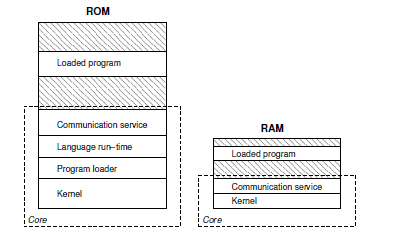
\includegraphics[width=0.9\textwidth]{Systemarchitektur_Contiki.png}
	\caption{Komponenten von Contiki \cite{Dunkels:Groenvall:Voigt:2014:Online}}
	\label{Systemarchitektur von Contiki}
\end{figure}
Der Core ist ein Basissystem und besteht aus dem Kernel, Bibliotheken, Ger\"{a}tetreibern und dem Programm-Lader. 
Im allgemeinen sind \"Anderungen am Core nicht vorgesehen und nur unter Verwendung eines speziellen Bootloaders m\"oglich. 
Die konkrete Aufteilung des Systems in Core und ladbare Programme wird beim Kompilieren des Systems entschieden und h\"angt 
von der Hardware-Plattform ab \cite[vgl.][S. 7]{Walter:2010}. Ger\"atetreiber werden als Bibliotheken implementiert. 

\paragraph{Events}
In Contiki kommunizieren Prozesse \"uber Events. Auch der Kernel versendet Events, um Prozesse \"uber ihren Status 
(Init, Continue, Exit) oder \"uber abgelaufene Timer zu Informieren. Zur Identifikation stehen dabei Event IDs zur 
Verf\"ugung. Die Event IDs 0-127 k\"onnen vom Benutzer frei vergeben werden, w\"ahrend die Prozess IDs ab 128 vom 
System genutzt werden. Grunds\"atzlich unterscheidet Contiki zwischen synchronen und asynchronen Events. 
\begin{itemize}
\item \textbf{Asynchrone Events} sind eine Form der Deferred Procedure Call: asynchrone Events werden vom Kernel in einer 
Warteschlange gespeichert. Die Scheduling-Funktion des Kernels l\"auft nach Systemstart in einer Endlosschleife. 
In jedem Durchlauf wird ein Event aus der Schlange entnommen und wird einige Zeit sp\"ater an den Zielprozess weitergeleitet.
\item \textbf{Synchrone Events} gleichen einem Funktionsaufruf.
Sie werden ohne Umweg \"uber die Warteschlange direkt an den Empf\"anger-Prozess
zugestellt \cite[vgl.][S. 7]{Walter:2010}.  Mit der Funktion process\_post\_synch(\&example\_process, EVENT\_ID, msg) wird gezielt ein 
Prozess aufgerufen (ein Broadcast ist nicht m\"oglich). W\"ahrend der aufgerufene Prozess aktiv ist, blockiert der Aufrufer und 
setzt seine Ausführung erst fort, wenn der aufgerufene Prozess die Kontrolle wieder abgibt.
\end{itemize}

\paragraph{Prozesse}
Prozesse in Contiki implementieren ein Konzept namens Protothreads. Dies erlaubt es Prozessen, ohne den Overhead und die langen 
Prozesswechselzeiten von normalen Threads auszukommen. Gleichzeitig k\"onnen trotzdem andere Prozesse ausgef\"uhrt werden, falls ein Prozess auf ein Event (Timer, Nachricht von anderem Prozess...) warten muss.
F\"ur die Entwicklung mit Prozessen ist wichtig, dass nicht-statische Variablen nicht zwischen zwei Aufrufen erhalten bleiben.
Der relevante Status eines Prozesses sollte daher mithilfe von statischen Variablen abgelegt werden (siehe Variable i im folgenden Beispiel)

\begin{figure}[h!]
	\centering
		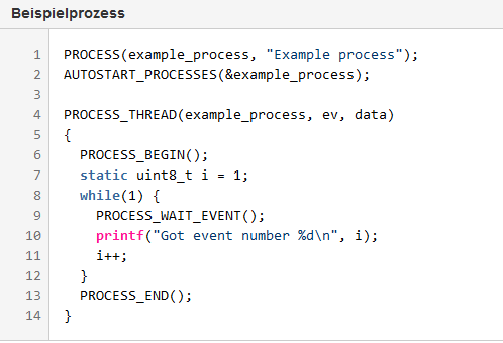
\includegraphics[width=0.9\textwidth]{Beispielprozess.png}
	\label{Beispielprozess}
\end{figure}
In Zeile 1 wird der Prozess initialisiert und in Zeile 2 automatisch beim Boot von Contiki gestartet. Zeile 4 beinhaltet die
Deklaration. So k\"onnen andere Prozesse diesem Prozess Events (mit oder ohne Daten) schicken, auf die unser Beispielprozess 
mit ev und data zugreifen kann. Zeile 6 kennzeichnet den Beginn der tats\"achlichen Ablauflogik. Code \"uber dieser Zeile wird 
bei jedem Prozessaufruf ausgef\"uhrt, dies wird jedoch in den meisten F\"allen nicht ben\"otigt. Zeile 13 schlie{\ss}lich beendet
den Prozess und entfernt ihn aus der Prozess-Liste des Kernels. In diesem Beispiel wird die Zeile jedoch nie erreicht, sodass der Prozess immer wieder aufgerufen wird, bis er von einem anderen Prozess beendet wird.
Wichtige Funktionen in Prozessen:
\begin{itemize}
\item PROCESS\_WAIT\_EVENT() - Wartet auf ein beliebiges Event, bevor die Ausf\"{u}hrung fortgesetzt wird.
\item PROCESS\_WAIT\_EVENT\_UNTIL(condition) - Wartet auf ein beliebiges Event, setzt die Ausf\"{u}hrung aber nur fort, wenn die Bedingung erf\"{u}llt ist.
\item PROCESS\_WAIT\_UNTIL() - Wartet, bis die Bedingung erf\"ullt ist. Muss den Prozess nicht zwangsl\"{a}ufig anhalten.
\end{itemize}
Prozesse k\"onnen \"uber Events (siehe Events) oder Polling-Anfragen kommunizieren.  Polls sind Events mit hoher Priorit\"at und 
k\"onnen genutzt werden, um den angerufenen Prozess so schnell wie m\"oglich auszuf\"uhren. Sie
sind besonders bei der Abarbeitung von Hardware-Interrupts wichtig, da Interrupts-Handler keine Events, sondern nur
Polling-Anfragen absetzten d\"urfen \cite[vgl.][S. 7]{Walter:2010}.

\subsubsection{Background Level: Treiber, Services und Interfaces}
Im Background Level werden Teiber, die sich um die Schnittstellen/Pins des Controllers wie z.~B. Protokolle angeschlossener Devices\cite[S. 26]{Stasch:Hahn} kümmern, Services, deren Aufgabe es ist, die Funktionen der Treiber zu sinnvollen Einheiten zusammenzufassen, und schließlich Interfaces, die genutzt werden, um die Funktionen der Services dem AgentenRTE zur Verfügung zu stellen und gleichzeitig plattformabhängige Implementierungsdetails zu maskieren, implementiert \cite[S. 26]{Stasch:Hahn}. Im Laufe der Projektarbeit wurden unterschiedliche Treiber, Services und Interfaces entwickelt. Der folgende Abschnitt soll diese einzeln näher beleuchten.

\paragraph{Treiber Bolzen}
Folgende Funktionen werden im Treiber für die Bolzen bereitgestellt:
\begin{itemize}
  \item void BoltDriver\_init(void)
  \item void BoltDriver\_up(unsigned char boltv)
  \item void BoltDriver\_down(unsigned char boltv)
  \item uint8\_t BoltDriver\_get(void)
\end{itemize} 
Die Funktion \textit{void BoltDriver\_init(void)} dient zur Initialisierung. Dabei werden die Ports der \textsc{Mica}z-Module, die für die Bolzensteuerung nötig sind, als Ausgänge festgelegt und gleichzeitig auf HIGH-Aktiv gesetzt.

Zum Öffnen der Bolzen wird die Funktion \textit{void BoltDriver\_down(unsigned char boltv)} genutzt. Ihr wird ein Vektor übergeben, der die Pinbelegung von den zu öffnenden Bolzen enthält. Da die Bolzen beim öffnen jeweils eine Anfansspannung von 24 Volt benötigen, muss darauf geachtet werden, dass die Bolzen nacheinander geöffnet werden. Im ersten Schritt fragt die Funktion ab, ob Bolzen 1 geöffnet werden soll. Bei erfolgreicher Prüfung, werden Pin 1 und 2 der ersten Bolzen angeschaltet, wodurch eine Anfangsspannung von 24 Volt anliegt und der Bolzen sich öffnen kann. Damit das Öffnen erfolgreich sichergestellt werden kann, wird dieser Zustand über 60 Taktzyklen gehalten, dann wird der zweite Pin wieder ausgeschaltet. Jetzt liegen über den angeschlossenen Verstärker noch 12 Volt Spannung an, was ausreicht um den Bolzen offen zu halten, ohne die Schaltung zu überhitzen. Im nächsten Schritt wird überprüft ob beide Bolzen gleichzeitig geöffnet werden sollen. Ist dies der Fall, dann wird wieder für 60 Taktzyklen im System gewartet. Im Anschluss daran wird kontrolliert, ob Bolzen 2 geöffnet werden soll. Liegt hier eine positive Bewertung vor, wird mit den Pins von Bolzen 2 analog zu Bolzen 1 vorgegangen.

Die Funktion \textit{void BoltDriver\_up(unsigned char boltv)} schließt die Bolzen. Dieser Funktion wird ebenfalls ein Vektor übergeben, der die Belegung der Bolzen enthält, die geschlossen werden sollen. Dabei wird geprüft, welche Bolzen geschlossen werden sollen. Anschließend werden dann jeweils beide Pins der Bolzen auf LOW gezogen, ein sukzessives \textit{Herunterfahren} der Spannung wie beim Öffnen ist nicht nötig.

Mit der Funkion \textit{uint8\_t BoltDriver\_get(void)} kann die Bolzenstellung abgefragt werden. Dabei wird einfach überprüft, ob die Ausgänge des \textsc{Mica}z-Modul an denen die Bolzen angeschlossen sind HIGH sind. Beim Rückgabevektor steht eine Eins im Vektor für einen offenen und eine Null für einen geschlossenen Bolzen.

\paragraph{Interface Bolzen}
Das Bolzen-Interface greift direkt auf die Treiber der Bolzen zu und stellt mehrere Funktionen zur Verfügung, durch die Prozesse gestartet werden. Die unterschiedlich bereitgestellten Funkionen im Bolzen-Interface sind:
\begin{itemize}
  \item void BoltInterface\_init(void);
  \item void BoltInterface\_release(void);
  \item void BoltInterface\_release\_and\_separate(void);
  \item void BoltInterface\_separate(void);
\end{itemize}

Durch die unteren drei Funktionen werden folgende Prozesse gestartet:
\begin{itemize}
  \item PROCESS\_NAME(bolt\_int\_release)
  \item PROCESS\_NAME(bolt\_int\_release\_and\_separate)
  \item PROCESS\_NAME(bolt\_int\_separate)
\end{itemize}

Der Prozess \textit{bolt\_int\_release} ist dafür zuständig, die untersten zwei Bolzen für einen bestimmten Zeitraum zu öffnen und dann wieder zu schließen. Dafür existieren zwei Zustände. Im ersten Zustand wird die Funktion \textit{BoltDriver\_up(unsigned char boltv)} aufgerufen. So wird sichergestellt, dass die oberen beiden Bolzen geschlossen sind, um nur exakt ein Paket freizugeben. Nach dem Aufruf der Funktion wird ein Timer gestartet. Zustand zwei ruft, sobald der Timer abläuft, die Funktion \textit{BoltDriver\_down(unsigned char boltv)} aus dem Treiber mit einem Vektor für die unteren beiden Bolzen auf und das Paket wird freigegeben. Im Anschluss daran, wird wieder ein Timeout gesetzt und gewartet. Nach dem Durchlauf der zwei Zustände wird vorm Prozessende die Funktion \textit{BoltDriver\_up(unsigned char boltv)} aus den Treibern aufgerufen, um die unteren Bolzen wieder zu schließen.

Um Pakete nicht nur von der Rampe auszugeben, sondern auch gleich das nächste Paket zu separieren, ist der Prozess \textit{bolt\_int\_release\_and\_separate} zuständig. Dabei werden zu Anfang des Prozesses vier unterschiedliche Zustände durchlaufen. Die ersten drei Zustände sind dafür da, das Paket von der Rampe zu entfernen. Hierbei wird genau wie oben beim der Funktion \textit{bolt\_int\_release} vorgegangen. Zustand vier wird im Anschluss daran dann benutzt, die oberen Bolzen wieder zu öffnen, damit das nächste Paket nachrutschen kann. Vorm Abschluss des Prozesses werden diese dannn wieder durch die Treiberfunktion \textit{BoltDriver\_up(unsigned char boltv)} geschlossen.

Mit dem dritten Prozess wird es ermöglicht, die oberen zwei Bolzen zu öffnen. Beim Prozessdurchlauf wird im Zustand eins sichergestellt, dass die unteren beiden Bolzen geschlossen sind. Im zweiten Zustand werden dann die oberen zwei Bolzen geöffnet, was ein Nachrutschen von Paketen ermöglicht. Bevor der Prozess dann beendet wird, werden die beiden Bolzen wieder geschlossen. Der Prozess ermöglicht es somit, ein Paket zu separieren.

\paragraph{Treiber Externer Speicher}
\label{sec:externalMemory}
Der Treiber für den externen Speicher setzt den SPI-Bus zum AT45DB041-Chip um. Dafür nutzt er die Pins D2 (RXD oder SO), D3 (TXD oder SI), D5 (SCK) und A3 (CS). Ein Befehl an den Speicher ist dabei stets gleich aufgebaut:
\begin{itemize}
\item 1 Byte Opcode
\item 4 Don't-Care-Bits und 11 Bit Seiten-Adresse
\item 9 Bit Buffer-Adresse
\item Read Trigger (nur für Lese-Befehle, Senden von ebenso vielen leeren Bytes wie empfangen werden sollen)
\end{itemize}

Der Treiber stellt folgende Funktionen zur Verfügung:

\begin{itemize}
  \item void ExtflashDriver\_init()
  \item uint8\_t ExtflashDriver\_tr\_byte(uint8\_t spiOut)
  \item void ExtflashDriver\_enable()
  \item void ExtflashDriver\_disable()
  \item void ExtflashDriver\_wait\_idle()
  \item uint8\_t ExtflashDriver\_read\_status\_register(void)
  \item uint8\_t ExtflashDriver\_get\_last\_compare(void)
\end{itemize}

Bemerkenswert ist hier insbesondere die Funktion \textit{ExtflashDriver\_tr\_byte}. Entsprechend des SPI-Busses sendet und empfängt sie gleichzeitig ein Byte vom Speicher.  \textit{ExtflashDriver\_wait\_idle} empfängt das erste Byte des Statusregisters. So kann geprüft werden, ob der Speicherchip gerade eine Seite in den Buffer lädt oder den Buffer zurückschreibt und deshalb mit dem nächsten Befehl gewartet werden muss \cite{AT45DB041A:2014:Online}.
\paragraph{Interface Externer Speicher}
Das Interface stellt für das Speicherinterface folgende Funktionen zur Verfügung:
\begin{itemize}
  \item void ExtflashInterface\_init()
  \item void ExtflashInterface\_restore(uint16\_t cell)
  \item void ExtflashInterface\_flush(uint16\_t cell)
  \item void ExtflashInterface\_agent\_restore(uint8\_t localAgentId)
  \item void ExtflashInterface\_agent\_flush(uint8\_t localAgentId)
  \item uint8\_t ExtflashInterface\_write(uint16\_t address, uint8\_t* data, uint8\_t len)
  \item uint8\_t ExtflashInterface\_read(uint16\_t address, uint8\_t* data, uint8\_t len)
\end{itemize}
\textit{ExtflashInterface\_restore} holt zwei aufeinanderfolgende Seiten (eine Zelle) aus dem Speicher und schreibt sie in den Buffer. \textit{ExtflashInterface\_flush(uint16\_t cell)} schreibt die beiden Seiten im Buffer an die angegebene Stelle im Speicher. \textit{ExtflashInterface\_agent\_restore} und \textit{ExtflashInterface\_agent\_flush} holen die Zelle eines bestimmten Agenten in den Speicher und schließlich sind \textit{ExtflashInterface\_write} und \textit{ExtflashInterface\_read} für Datenzugriffe im Buffer zuständig und können Daten lesen beziehungsweise schreiben.
\paragraph{Speicherinterface}
Das Speicherinterface stellt den Agenten den externen Flashspeicher zur Verfügung. Jedem Agenten werden dafür zwei Seiten zugeordnet. Ruft er nun die Funktionen \textit{MemoryInterface\_readComponentCell(uint8\_t componentCount, uint8\_t cell, uint8\_t* result, uint8\_t length)} oder \textit{MemoryInterface\_writeComponentCell(uint8\_t componentCount,uint16\_t cell, uint8\_t* data, uint8\_t length)} auf, wird geprüft, ob die Zelle des aktuellen Agenten bereits im Buffer ist. Falls nicht, werden die aktuellen Bufferdaten gesichert und es werden die Daten des aktiven Agenten geladen.
\paragraph{Treiber Lichtschranken}
Durch den Lichtschrankentreiber werden zwei Funktionen zur Verfügung gestellt. Zum einen ist es die Funktion \textit{void photosensor\_drv\_init(void)}. In dieser werden alle nötigen Eingänge der \textsc{Mica}z-Module initialisiert. Zum anderen wird durch den Treiber die Funktion \textit{uint8\_t get\_photosensors()} implementiert. Durch die Funktion kann der Zustand der Lichtschranken abgefragt werden. Dabei steht eine 1 für eine unterbrochene und eine 0 für eine offene Lichtschranke.

\paragraph{Interface Lichtschranken}
Über das Interface zur Lichtschranke werden folgende drei Funktionen bereitgestellt:
\begin{itemize}
  \item void PhotosensorInterface\_init(void)
  \item uint8\_t PhotosensorInterface\_is\_bay\_occupied(uint8\_t i)
  \item uint8\_t PhotosensorInterface\_num\_packages(void)
\end{itemize}
Durch die Funktion \textit{void PhotosensorInterface\_init(void)} werden die Lichtschranken über den Treiber initialisiert. Dafür wird lediglich die Funktion \textit{void photosensor\_drv\_init(void)} aus dem Treiber aufgerufen.

Die zweite oben aufgeführt Funktion wird genutzt, um zu überprüfen, ob eine bestimmte Lichtschranke unterbrochen wurde oder nicht. Dafür wird der Funktion ein Wert übergeben, der die zu überprüfende Lichtschranke enthält. Ist der übergebende Wert größe als vier, mehr Lichtschranken wurden nicht verbaut, oder kleiner als eins wird eine 0 zurückgegeben, was als nicht ausgelöste Lichtschranke zu interpretieren ist.

\paragraph{Treiber Funkmodul}
Der Treiber für das Funkmodul ist zuständig für die korrekte Funktionalität der drahtlosen Kommunikation zuständig und greift dafür auf den Contiki-Kommunikationsstack \textit{RIME} zu. Auf das Coktiki-interne Atomic Broadcast Protokoll wird durch den Treiber ein Networkflooding augesetzt, das eine zuverlässigere Nachrichtenübermittlung ermöglicht. Dabei werden folgende Funktionen zur Verfügung gestellt:\begin{itemize}
  \item void radio\_open(struct radio\_conn *c, uint16\_t channel, const struct radio\_callbacks *u)
  \item void RadioDriver\_sendmessage(uint8\_t* msgtext, uint8\_t length)
  \item void RadioDriver\_receivemessage(struct radio\_conn *c)
  \item void RadioDriver\_init(void)
\end{itemize}


\paragraph{Treiber UART-Schnittstelle}
Der UART-Treiber ermöglicht die Kommunikation der \textit{Mica}z-Module über den USB-Port. Dafür wurden vom Treiber die folgenden Funktionen entwickelt.
\begin{itemize}
  \item void UartDriver\_send(uint8\_t *buf, uint8\_t size)
  \item int UartDriver\_line\_input\_byte(unsigned char c)
  \item void UartDriver\_line\_init(void)
\end{itemize}
und zusätlich der Prozess
\begin{itemize}
  \item UartDriver\_recv\_process
\end{itemize}

Die Initialisierung der UART-Schnittstelle findet in der Methode \textit{void UartDriver\_line\_init(void)} statt. Dabei wird ein Ringbuffer, der für den Empfang der Zeichen zuständig ist, initialisert. Außerdem wird der für die Verarbeitung verantwortliche Prozess gestartet.

Die Funktion \textit{void UartDriver\_send(uint8\_t *buf, uint8\_t size)} wird für das Senden über die UART-Schnittstelle benötigt. Dabei wird ein Zeiger auf die Adresse der zusendende Nachricht und die Länge der Nachricht an die Funktion übergeben. Zu Anfang der Funktion wird geprüft, ob die zu sendende Nachricht kleiner als fünf Byte ist. Wenn die Nachricht kürzer als fünf Byte ist, dann wird die Nachricht mit Bytes mit dem Wert 0x00 aufgefüllt. Die Nachricht wird dann byteweise über die UART-Schnittstelle ausgegeben.

Die Methode \textit{int UartDriver\_line\_input\_byte(unsigned char c)} wird zum einlesen über die UART-Schnittstelle verwendet. Es handelt sich hierbei um einen Callback, der von einem Interrupt immer dann aufgerufen wird, wenn ein Byte empfangen wird. Dafür wird überprüft, ob ein Überlauf vorliegt. Wenn dies der Fall ist, wird das Zeichen komplett bis zum Zeilenende ignoriert und der Parameter für den Überlauf auf 0 gesetzt. Wenn genug Platz im Buffer vorhanden ist, wird das empfangene Zeichen eingelesen und im Buffer gespeichert. Kann das Zeichen nicht mehr gespeichert werden, wird der Parameter für den Überlauf auf 1 gesetzt. Zum Schluss wird der Prozess \textit{UartDriver\_recv\_process} gepollt. Dieser ist für die Verarbeitung der empfangenen Nachricht verantwortlich. Dabei wird das eingehende Byte in einen Buffer geschrieben. Wenn der Buffer eine Länge von fünf Byte hat, wird dieser an das Communication Interface weitergereicht.

\paragraph{Interface UART-Schnittstelle}
Durch das UART-Interfache werden folgende Funktionen zur Verfügung gestellt:
\begin{itemize}
  \item void UARTInterface\_drive\_to\_entry(uint16\_t rampid)
  \begin{itemize}
    \item Gibt den Befehl aus, zum Eingang der Rampe mit der Rampen-ID rampid zu fahren
  \end{itemize}
  \item void UARTInterface\_drive\_to\_exit(uint16\_t rampid)
  \begin{itemize}
    \item Gibt den Befehl aus, zum Ausgang der Rampe mit der Rampen-ID rampid zu fahren
  \end{itemize}
  \item void UARTInterface\_how\_cost\_job(uint16\_t startid, uint16\_t targetid)
  \begin{itemize}
    \item Stellt die Frage, wie hoch die Kosten sind ein Paket von Startrampe (startid) zur Zielrampe (targetid)
  \end{itemize}
  \item void UARTInterface\_give\_package(void)
  \begin{itemize}
    \item Befehl Paket an die Rampe abzugeben
  \end{itemize}
  \item void UARTInterface\_take\_package(void)
  \begin{itemize}
    \item Befehl Paket von Rampe entgegenzunehmen
  \end{itemize}
\end{itemize}
Alle Funktionen sind dazu nötig um Befehle an die Teilgruppe Drive zusenden. Mit diesen können Nachrichten an den Volksbot über die USB-Schnittstelle versandt werden.

\subsubsection{Agenten RTE}
\label{sec:AgentRTE}
Auf der nächsten Hierarchieebene über den Interfaces liegt die Laufzeitumgebung der Agenten (AgentRTE). Es ist die erste plattformunabhängige Ebene über den Interfaces und dem Betriebssystem. Vergleicht man die Implementation für STASH-Controller und \textsc{Mica}z-Module, unterscheidet sich das AgentenRTE lediglich im Prozessmodell der Agenten, das abhängig vom Betriebssystem ist: Während die STASH-Controller mit dem MSP430-Mikrocontroller auf SYS/BIOS mit präemptivem Scheduling stetzen, läuft auf den \textsc{Mica}z-Modulen ein nicht-präemptives Contiki-System. Die Agenten auf den Stash-Controllern werden daher jeweils durch einen eigenen Prozess repräsentiert, während es auf den \textsc{Mica}z-Modulen einen gemeinsamen Prozess gibt, der Agenten über Funktionszeiger aufruft. Wir gehen hier nur auf die Implementierung auf den \textsc{Mica}z-Modulen ein.

Neben dem Aufruf der einzelnen Agenten ist das AgentenRTE auch für das Registrieren und Terminieren der Agenten und den Austausch beziehungsweise die Verteilung von Nachrichten verantwortlich.

\paragraph{Verwaltung der Agenten}\mbox{}\\
Agenten werden mit ID und Typ registriert. Nach Konvention bekommt dabei der Plattform-Agent stets die ID des Moduls, der Order-Agent eine um eins erhöhte ID und der Routing-Agent eine um zwei erhöhte ID. Hat Beispielsweise das Modul die ID \textit{0x0110}, so hat der Plattform-Agent ebenfalls die ID \textit{0x0110}, der Order-Agent die ID \textit{0x0111} und der Routing-Agent schließlich die ID \textit{0x0112}. Die Registrierung dieser Agenten erfolgt in der Main-Methode des Systems. Die Nummerierung der Paket-Agenten ist unabhängig von dieser Konvention, allerdings muss darauf geachtet werden, dass ihre IDs nicht mit den übrigen Agenten übereinstimmen.

Registrierte Agenten werden in ein Array aus Agenten-Strukturen eingetragen und dort verwaltet.
\autoref{lst:agentstruct} zeigt die Agenten- und Agenten-Callback-Strukturen. Außerdem wird einmalig ihre Init-Methode aufgerufen.

Bei der Ausführung wird nun bei jedem Prozessaufruf des Agenten-Prozesses eine Zählervariable erhöht, die jeweils die Main-Methode des nächsten Agenten aufruft. Da  Contiki ein nicht-präemptives Scheduling nutzt, dürfen die Agenten nicht blockieren, sondern müssen die Kontrolle an den Haupt-Prozess zurückgeben, sprich die Main-Methode muss terminieren.

\lstinputlisting[language=C, style=customc, captionpos=b, caption={Agenten Strukturen in C}, label=lst:agentstruct]{src/flow/lst/agent_struct.lst}

\paragraph{Austausch von Nachrichten}\mbox{}\\
Der Austausch von Nachrichten und damit die Kommunikaion zwischen Agenten ist unerlässlich in einem Multiagentensystem. Auch diese Aufgabe kommt dem AgentenRTE zu. Die Laufzeitumgebung prüft den Empfänger einer Nachricht und übergibt sie schließlich an den richtigen Agenten. Der Aufbau einer solchen Agenten-Nachricht wird durch eine Struktur beschrieben, die in \autoref{lst:commsg} abgebildet ist. Der Kopf einer Nachricht ist demnach 15 Byte groß, die Nutzdaten können bis zu 26 Byte betragen.

\lstinputlisting[language=C, style=customc, captionpos=b, caption={Struktur einer Agenten-Nachricht in C}, label=lst:commsg]{src/flow/lst/message_struct.lst}

Sendet ein Agent eine solche Nachricht, übergibt er sie dem AgentRTE. Dieses prüft, ob sich der Empfänger-Agent auf dem eigenen Modul befindet. Ist das der Fall, wird die Nachricht in der Warteschlange für eingehende Nachrichten gespeichert und kann dort vom Empfänger abgerufen werden. Wenn der Agent nicht auf der Plattform registriert ist, wird die Nachricht an das CommunicationInterface weitergeleitet, das sich zum die Verteilung im Netzwerk kümmert. So gelangt die Nachricht auch über die Modulgrenzen hinweg zum richtigen Agenten.

Eingehende Nachrichten werden vom CommunicationInterface an das AgentRTE weitergereicht. Dafür wird zunächst angefragt, ob sich der Ziel-Agent beziehungsweise einer der Ziel-Agenten im Falle von Gruppennachrichten auf der Plattform befindet. Ist dies der Fall wird die Nachricht in der Warteschlange für eingehende Nachrichten gespeichert.

Ein großes Problem bei Nachrichtenaustausch stellt der mit 4 KB sehr begrenzte Arbeitsspeicher der \textsc{Mica}z-Module dar. Entsprechend ist der Platz in der Warteschlange für eingehende Nachrichten begrenzt, pro Agent können nur drei Nachrichten gespeichert werden. Um den Speicher nicht überlaufen zu lassen und dadurch Nachrichten zu verlieren, wird daher das Senden von Nachrichten durch ein Token-System begrenzt. Pro Agent kann so in jedem Durchlauf nur eine Nachricht versendet werden. Nutzt ein Agent dies nicht aus, kann sein Token auf einen anderen Agenten übertragen werden. In der Praxis schränkt diese Restriktion die Agenten in ihrer Funktionalität jedoch nicht ein. Meist erfordert eine eingehende Nachricht nur eine direkt Antwort oder die Benachrichtigung eines anderen Agenten. Müssen einmal doch zwei oder mehr Nachrichten als Reaktion versendet werden, geschieht dies mithilfe von Zwischenzuständen und Flags, die beim nächsten Durchlauf aktiv werden.
%\begin{figure}[h!]
%	\centering
%		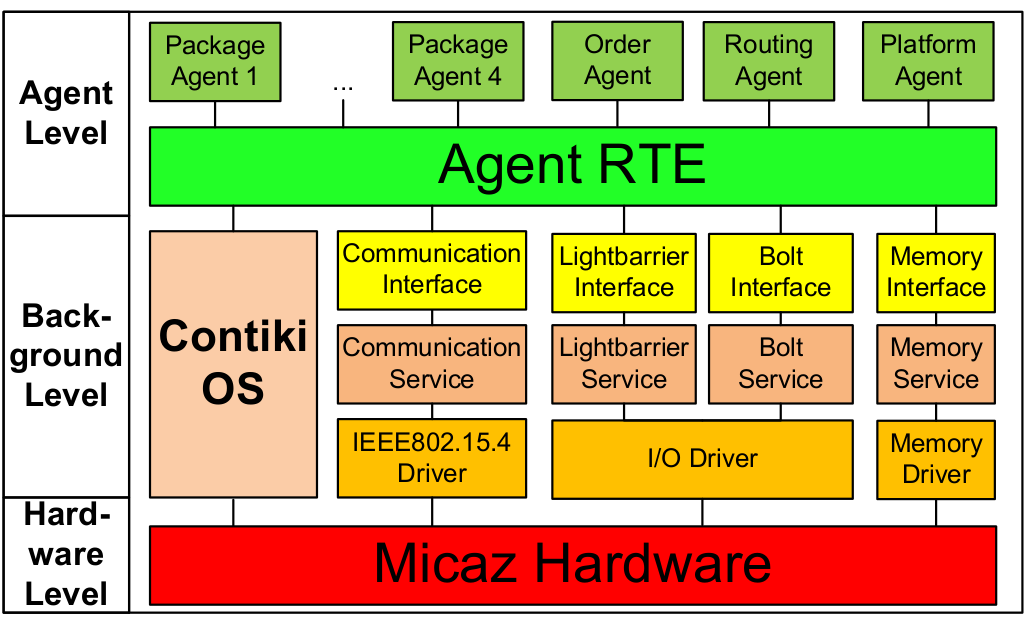
\includegraphics[width=0.9\textwidth]{ArchitekturMicazRampe.png}
%	\caption{Architektur Micaz Rampe\cite{Stasch:Hahn}}
%	\label{ArchitekturMicazRampe}
%\end{figure}

\subsection{Agenten}
Oberhalb des AgentRTE sind die Agenten implementiert. Sie bilden die oberste Ebene des Systems und implementieren die eigentliche Funktionalität. Dabei greifen sie auf das AgentenRTE und die verschiedenen Interfaces zu und kommunizieren untereinander über Agenten-Nachrichten. Auf jedem Modul agieren ein Plattform-Agent, der die Sensoren und Aktoren der Plattform steuert, ein Order-Agent, der zusammen mit anderen Order-Agenten die Betriebslogik des Materialflusssystems darstellt, ein Routing-Agent, der gemeinsam mit anderen Routing-Agenten die Pakete durch das System leitet und eventuell bis zu vier Paket-Agenten, die die physischen Pakete repräsentieren und durch das System wandern. Die einzelnen Agenten sind im Folgenden beschrieben.
\subsubsection{Paket-Agent}
Ein Paket Agent repräsentiert ein physisches Paket. Seine ID ist gleichzeitig auch Paketnummer. Beim Eintritt im System wird vom Plattform-Agent ein neuer Paket-Agent initialisiert. Wechselt ein Paket von einem Modul auf das nächste, so wandert auch der Paket-Agent auf das neue Modul. Dies wird erreicht, indem der Agent auf dem einen Modul beendet und auf dem nächsten mit seinem Ziel und seiner ID neu initialisiert wird. Dies ist möglich, da sich verschiedene Pakete nur durch ihr Ziel und ihre ID voneinander unterscheiden. Die Übertragung der Paket-Agenten wird von den Plattform-Agenten der jeweiligen Module übernommen.

Das Ziel von Paket-Agenten ist dynamisch. Es wird von den Order-Agenten verwaltet. Kommt ein neuer Auftrag ins System, wird vom Order-Agenten, der den Auftrag verwaltet, eine Nachricht an das entsprechende Paket gesendet. Erhält der Paket-Agent eine solchen Nachricht, wird dem Order-Agenten der Empfang bestätigt und das eigene Ziel wird angepasst.

Hat der Paket-Agent ein gültiges Ziel und wird ihm vom Plattform-Agenten per Flag die Erlaubnis erteilt, sendet er dem Routing-Agenten seiner Plattform eine Routing-Anfrage, bestehend aus dem Ziel des Pakets. Wenn diese nicht abgelehnt wird, wartet der Paket-Agent, bis sein Ziel geändert wird, oder sich auf einer Plattform befindet, die nicht seinem aktuellen Ziel entspricht und er die erneute Erlaubnis bekommt, eine Routing-Anfrage zu stellen. Wird die Anfrage dagegen abgelehnt, stellt er beim nächsten Aufruf eine neue, bis die Anfrage vom Routing-Agenten angenommen wird.

Schließlich kann der momentane Zustand des Pakets über eine sogenannte \textit{UPDATE\_PHYSICAL}-Nachricht von einem Gateway abgefragt werden. Der Agent antwortet darauf mit der ID der Plattform, auf der er sich zur Zeit befindet und dem eigenen Ziel.
\subsubsection{Plattform-Agent}
Der Plattform-Agent ist der einzige plattformabhängige Agent des Systems. Während alle anderen Agenten auf allen Modultypen identisch sind, ist der Plattform-Agent modulspezifisch. Seine Aufgabe ist die Steuerung und Überwachung seines Moduls.

Beiden gemeinsam ist jedoch die Übertragung, also das Beenden und die erneute Initialisierung, von Paket-Agenten. Diese wird immer vom Volksbot initialisiert. Es wird eine Anfrage an den Plattform-Agenten der jeweiligen Rampe gesendet, entweder nach einem Lagerplatz oder nach einem speziellen Paket, abhängig davon, ob ein Paket abgelegt oder aufgenommen werden soll. Soll ein Paket abgelegt werden, muss die Anfrage bestätigt werden, bevor ein Registrierungs-Auftrag mit den Details des Paket-Agenten gesendet wird und der Agent auf seiner momentanen Plattform terminiert wird. Soll ein Paket aufgenommen werden, prüft die Rampe, ob das Paket mit der geforderten ID vorhanden ist und ausgegeben werden kann und sendet im Erfolgsfall ebenfalls einen Registrierungs-Auftrag und terminiert seinerseits den  entsprechenden Paket-Agenten, der dann auf dem Volksbot neu initialisiert wird.

Außerdem geben beide auf eine \textit{UPDATE\_PHYSICAL}-Nachricht die IDs aller Paket-Agenten zurück, die sich derzeit auf dem Modul befinden.

Im Folgenden werden nun die plattformspezifischen Eigenschaften der Plattform-Agenten beschrieben.

\paragraph{Plattform-Agent der Rampen}\mbox{}\\
Der Plattform-Agent auf einer Rampe ist neben der Verwaltung der Paket-Agenten auch für die Steuerung und das Auslesen der Bolzen über das Bolt\_Interface beziehungsweise Lichtschranken über das Photosensor\_Interface verantwortlich. Er sorgt dafür, dass die Pakete korrekt vereinzelt werden und verwaltet ihre Reihenfolge. Außerdem prüft er auf die Anfrage eines Volksbots, ein Paket abzulegen, anhand der Lichtschranken, ob noch ein Platz auf der Rampe zur Verfügung steht.
\paragraph{Plattform-Agent der Volksbots}\mbox{}\\
Der Plattform-Agent auf einem Volksbot kommuniziert mit dem Laptop, der den Volksbot steuert. Er erhält eine Nachricht, wenn der Volksbot seine Ziel-Position erreicht hat. Daraufhin initiiert er die Übergabe des Paketes. War die Übergabe des Paket-Agenten erfolgreich, sendet der dem Laptop eine Nachricht über die serielle UART-Nachricht um das Fließband auf dem Volksbot zu starten und die physische Übernahme des Pakets zu starten.
\subsubsection{Order-Agent}
Die Order-Agent übernehmen die Rolle eines zentralen Materialflussrechner im Materialflusssystem. Ihre Aufgabe ist die Verarbeitung von Aufträgen, sprich die Zuweisung von Zielen an Pakete. Aufträge bestehen aus Paket- und Ziel-ID und werden über ein Gateway in das System eingegeben. Dafür wird eine entsprechende Agenten-Nachricht an einen einzelnen Order-Agenten gesendet, der den Empfang bestätigt oder ablehnt, falls kein Platz in seinem Speicher zur Verfügung stand. In diesem Fall muss ein anderer Order-Agent mit dem Auftrag betraut werden. Ein Auftrag wird mit seiner Paket- und Ziel-ID sowie einem Status ("zu bearbeiten" beziehungsweise "in Verteilung") in einer Warteschlange ablegt.

Hat der Order-Agent in einem Aufruf keine Nachricht erhalten, durchsucht er diese Warteschlange nach zu bearbeitenden Aufträgen und sendet eine Nachricht an das entsprechende Paket, sein Ziel zu ändern. Wird der Empfang dieser Nachricht vom Paket bestätigt, wird der Auftrag gelöscht, von nun an ist das Paket für die Erreichung seines Ziels verantwortlich. Sind alle Aufträge in Verteilung muss davon ausgegangen werden, dass die entsprechenden Nachrichten nicht angekommen sind oder die Pakete noch nicht im System sind. Daher wird in diesem Fall der Status aller Aufträge zurückgesetzt und es wird erneut versucht, Nachrichten an die einzelnen Pakete zu senden.
\subsubsection{Routing-Agenten}

Die Routing-Agenten kümmern sich um die Wegplanung der Pakete im Materialflusssystem. Sie suchen nach einem Volksbot, der ein Paket mit möglichst günstig zu seinem Ziel bringen kann. Dafür führen sie untereinander eine Auktion durch, bei der ein Transportauftrag zu möglichst geringen Kosten an einen Volksbot vergeben wird. Ein Routing-Agent reagiert dabei auf die Routing-Anfrage eines Paket-Agenten. Ein Routing-Agent kann gleichzeitig nur an einer Auktion teilnehmen beziehungsweise diese initiieren. Hiermit wird verhindert, dass ein Routing-Agent gleichzeitig zwei Auktionen gewinnt und deshalb eine der Auktionen zurückgerollt und wiederholt werden muss.

Die Routing-Agenten werden als kommunizierende Zustandsautomaten implementiert. Zustandsübergänge können durch eingehende Nachrichten oder Timer ausgelöst werden. \autoref{fig:routing_agent_fsm} zeigt den zugrunde liegenden Automaten.

\begin{figure}[h!]
  \centering
    \includegraphics[width = 1.35\textwidth, angle=90]{flow/RoutingAgent_FSM.png}
    \caption{Zustandsautomat des Routing Agenten}
    \label{fig:routing_agent_fsm}
\end{figure}

Ein Routing-Agent startet stets in Zustand 0. In diesem Zustand wartet er auf eingehende Routing-Anfragen. Diese können entweder von Paketen auf der eigenen Plattform oder von anderen Routing-Agenten kommen. Sie unterscheiden sich im ersten Byte der Conversation-ID einer Agenten-Nachricht. Hier ist die Autkions-ID gespeichert, die für neue Routing-Anfragen von Paketen erst durch den Routing-Agenten bestimmt werden muss und daher auf 0 gesetzt ist. 

Bei Eingang einer Routing-Anfrage durch ein Paket wird eine neue Routing-Anfrage an alle Routing-Agenten versendet, ein Timer gestartet, der abläuft, wenn die Bearbeitungszeit  und in Zustand 3 übergegangen. Kommt die Anfrage von einem anderen Routing-Agenten prüft der Agent, ob das Ziel erreichbar ist. Für Module auf einem Volksbot ist dies immer wahr, für Module an Rampen immer falsch. Ist das Ziel erreichbar, wird eine UART-Nachricht an den Volksbot gesendet, der die Kosten der Fahrt vom anfragenden Routing-Agenten zum Ziel des Pakets berechnen soll. Anschließend geht der Automat in Zustand 1 über.

In Zustand 1 wartet der Agent auf die Antwort des Volksbots auf seine Kostenanfrage. Geht diese ein und sind die Kosten größer als null, bedeutet dies, das Ziel ist erreichbar. Der Agent sendet anschließend diese Kosten an den Initiator der Auktion und geht in Zustand 2 über, wo er auf die Antwort des Initiators wartet. Wird das Angebot bestätigt, wird der Volksbot beauftragt, sich zum Ausgang des Initiators zu bewegen und der Automat geht in Zustand 6 über. Wird die Anfrage abgelehnt, geht der Automat zurück in Zustand 0 und wartet auf neue Anfragen. In Zustand 6 wartet der Routing Agent auf eine Nachricht des Plattform-Agenten, der bestätigt, dass das Paket abgegeben wurde und neue Anfragen angenommen werden können.

In Zustand 3 wartet der Routing-Agent auf Angebote von anderen Routing-Agenten, nachdem er eine Routing-Anfrage für ein Paket auf der eigenen Plattform verschickt hat. Er speichert diese Angebote mit Absender-ID und Kosten. Läuft schließlich der Bearbeitungs-Timer ab, wird geprüft ob mindestens ein Angebot eingangen ist. Ist das der Fall, wird das beste Angebot bestimmt und der Agent geht in Zustand 4 über. Andernfalls wird ein neuer Timer gesetzt, bis die Anfrage wiederholt wird und der Agent geht in Zustand fünf. In Zustand 5 wartet der Agent auf den Ablauf des Timers, versendet die Routing-Anfrage erneut an alle Routing-Agenten und geht zurück in Zustand 3. Zustand 4 dagegen bleibt aktiv, bis alle Teilnehmer der Auktion benachrichtigt wurden. In jedem Aufruf des Agenten wird eine Nachricht mit Cancel oder Acknowledge an einen weiteren Teilnehmer der Auktion gesendet. Sind alle Teilnehmer benachrichtigt, geht der Agent zurück in Zustand 0 und wartet auf neue Anfragen.


\subsection{Validierung}

\subsubsection{Erreichte Funktionalität}

\subsubsection{Probleme und Herausforderungen}

\subsubsection{Ausblick}


	
		% Chapter 7 Teilberichtfarhrzeug
	\clearpage
	\ohead[Teilberichtfarhrzeug]{Teilberichtfarhrzeug}
	\chead[Uni Oldenburg]{Uni Oldenburg}
	\ihead[PG FAISE]{PG FAISE}
	\setheadtopline{1pt}
	\setheadsepline{0.5pt}
	\ofoot[Endbericht]{Endbericht}
	\cfoot[\pagemark]{\pagemark}
	\ifoot[30. September 2014]{30. September 2014}
	\setfootsepline{0.5pt}
	\setfootbotline{1pt}
	\section{Teilbericht Fahrzeuge}

Ziel der Teilgruppe Fahrzeuge ist es, einen autonomen Transport zwischen den Rampen zu realisieren. Dafür sollen die Volksbots in der Lage sein, auf die eingehenden Aufträge zu reagieren.
Dies beinhaltet die Teilnahme an Auktionen ( Jobverteilung ), welche durch eine Aufwandsabschätzung des Auftrages eines jeden Volksbots entschieden werden. Nach der Zuweisung an den besten geeigneten Volksbot soll dieser das Paket von der entsprechenden Startrampe holen und zur Zielrampe transportieren.


Folgendes wird in den nächsten Unterkapiteln behandelt:

\begin{itemize}
	\item Anforderungskatalog an das Endsystem
	\item Beschreibung der Komponenten
	\item Werkzeuge
	\item Architektur
	\item Implementierung
	\item Erreichte Funktionalitäten
	\item Herausforderungen
	\item Ausblick
\end{itemize} 


\subsection{Anforderungen}
In diesem Abschnitt werden die gestellten Anforderungen zusammengetragen. Wir unterscheiden dabei zwischen funktionalen Anforderungen, die die direkte Funktionalität des fertigen Systems beschreiben, und nicht-funktionalen Anforderungen, die die qualitativen Eigenschaften des Systems widerspiegeln.
\subsubsection{Funktionale Anforderungen}
\begin{enumerate}
\item \textbf{Plattform}: Die physische Zelle wird als Netzwerk von Knoten in einem drahtlosen Sensornetzwerk implementiert. Als Plattform dienen MICAz-Module mit Atmel ATMega 128 Mikrocontroller und CC2420 Funkchip (siehe \autoref{MICAZ}).
 \item \textbf{Aktorik/Sensorik}: Die Rampen verfügen über Magnetstifte zum Vereinzeln der Pakete und Lichtschranken zum Erkennen von Paketen. Sie werden von den MICAz-Modulen angesteuert beziehungsweise ausgelesen.
 \item \textbf{Kommunikation}: Die MICAz-Module auf Rampen und Volksbots kommunizieren drahtlos untereinander auf Basis von Agenten-Nachrichten.
 \item \textbf{Synchronisation}: Die Simulation wird über ein Micaz-Modul, das als Gateway fungiert, an die drahtlose Kommunikation angebunden. Die Synchronisation der Zustände erfolgt über eine serielle Schnittstelle.
 \item \textbf{Disposition}: Die Controller kennen den Belegungszustand der Rampe und generieren nach dem FIFO-Prinzip Aufträge, die sie an die Volksbots vergeben.
 \item \textbf{Übergabe}: Wenn eine Ein- oder Auslagerung an einer Rampe ausgeführt werden soll, so übernimmt der Controller der Rampe die Kontrolle über die Fördereinheit des Fahrzeugs und sorgt dafür, dass das Paket verladen wird.
 \item \textbf{Kooperation}: Einsatz kooperativer Lösungsstrategien für die Materialflusssteuerung, Überwachung und Steuerung mittels Multi-Agentensystem.
\end{enumerate}

\subsubsection{Nicht-funktionale Anforderungen}
\begin{enumerate}
\item \textbf{Ressourcen}: Bei der Entwicklung muss 
auf den sparsamen Umgang mit Hardwareressourcen (Rechenzeit, Kommunikationsbandbreite, Speicher) geachtet werden. Insbesondere der vorhandene Arbeitsspeicher und das Kommunikationsmedium dürfen nicht überlastet werden, um einen stabilen Betrieb zu garantieren. 
\item \textbf{Stabilität}: Es müssen Maßnahmen getroffen werden, um ein stabiles System zu schaffen. Dies gilt insbesondere für die möglichst verlustfreie Übertragung von drahtlosen Nachrichten.
\item \textbf{Volksbots}: Die Module des Materialfluss über eine definierte Schnittstelle mit den Fahrzeugen kommunizieren, um auf die Aktorik und Sensorik der Volksbots zugreifen und schließlich einen Transport der Pakete gewährleisten zu können.
\end{enumerate}

\subsection{Beschreibung der Komponenten}
Dieser Abschnitt beschreibt die physikalischen Komponenten, die von der Teilgruppe Materialfluss verwendet wurden. Zu den diesen Komponenten zählen die Rampen, sowie die \textsc{Mica}z-Module mit ihren Mikrocontrollern. 
\subsubsection{Rampen}
Rampen stellen Ein- und Ausgänge, sowie Zwischenlager im physischen System dar. Auf einer Rampe finden bis zu vier Pakete Platz. Bolzen hinter dem ersten Paket, separiert dieses von den anderen Dreien. Damit das vorderste Paket nicht vorne von der Rampe herunterfällt, sind an der Vorderseite zwei weitere Bolzen angebracht. 

Durch vier Lichtschranken, wird eine Überwachung der Rampe ermöglicht. Diese beinhaltet zum einen das Abfragen, wie viele Pakete auf einer Rampe liegen. Zum anderen kann durch die Überwachung überprüft werden, an welcher Stelle Pakete liegen.

Alle vier Bolzen sind seitlich der Rampe befestigt. Eine autonome Steuerung der Rampen, wird durch ein angebrachtes \textsc{Mica}z-Modul ermöglicht.
\autoref{fig:skiram} zeigt ein Beispiel solch einer Rampe.

\begin{figure}[h!]
	\centering
		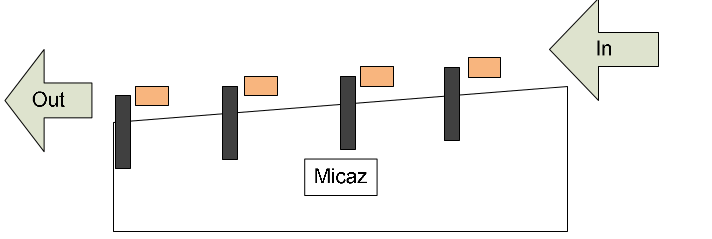
\includegraphics[width=0.9\textwidth]{SkizzeRampe.png}
	\caption{Beispiel einer eingesetzten Rampe}
	\label{fig:skiram}
\end{figure}

\subsubsection{Mikrocontroller}
Ein Mikrocontroller ist ein vollständiger Kleinstrechner auf einem einzigen Chip, dessen Zentraleinheit aus einem oder mehreren Mikroprozessen besteht. Zusätzlich enthält ein Mikrocontroller Speicher und Ein- bzw. Ausgabeschnittstellen zur Außenwelt. Dazu können neben einfach Ausgangspins auch komplexere Busprotokolle wie etwa USART, SPI oder CAN gehören.

Mikrocontroller werden eingesetzt, wenn eine Kommunikations- oder Steuerungsaufgabe mit möglichst geringen Ressourcen (Baugröße, Energie, Kosten) gelöst werden müssen. Die in einem Mikrocontroller verbauten Prozessorkern, Speicher und die Aus- und Eingabeschnittstellen, sind auf die Lösung derartiger Aufgaben zugeschnitten. Die große Anzahl an potenziellen Aufgabenstellungen hat zur Folge, dass es eine Vielfalt von Mikrocontrollern gibt. Meist sind die Mikrocontroller deshalb in Mikrocontrollerfamilien aufgeteilt. Innerhalb einer Familie unterscheiden sich die Controller nicht im Prozessorkern, sondern im verfügbaren Speicher und in den Ein- und Ausgabeschnittstellen \cite{ECHT2005}. In \autoref{fig:aufbmc} ist der schematische Aufbau eines MCs dargestellt.
\begin{figure}[th]
	\centering
		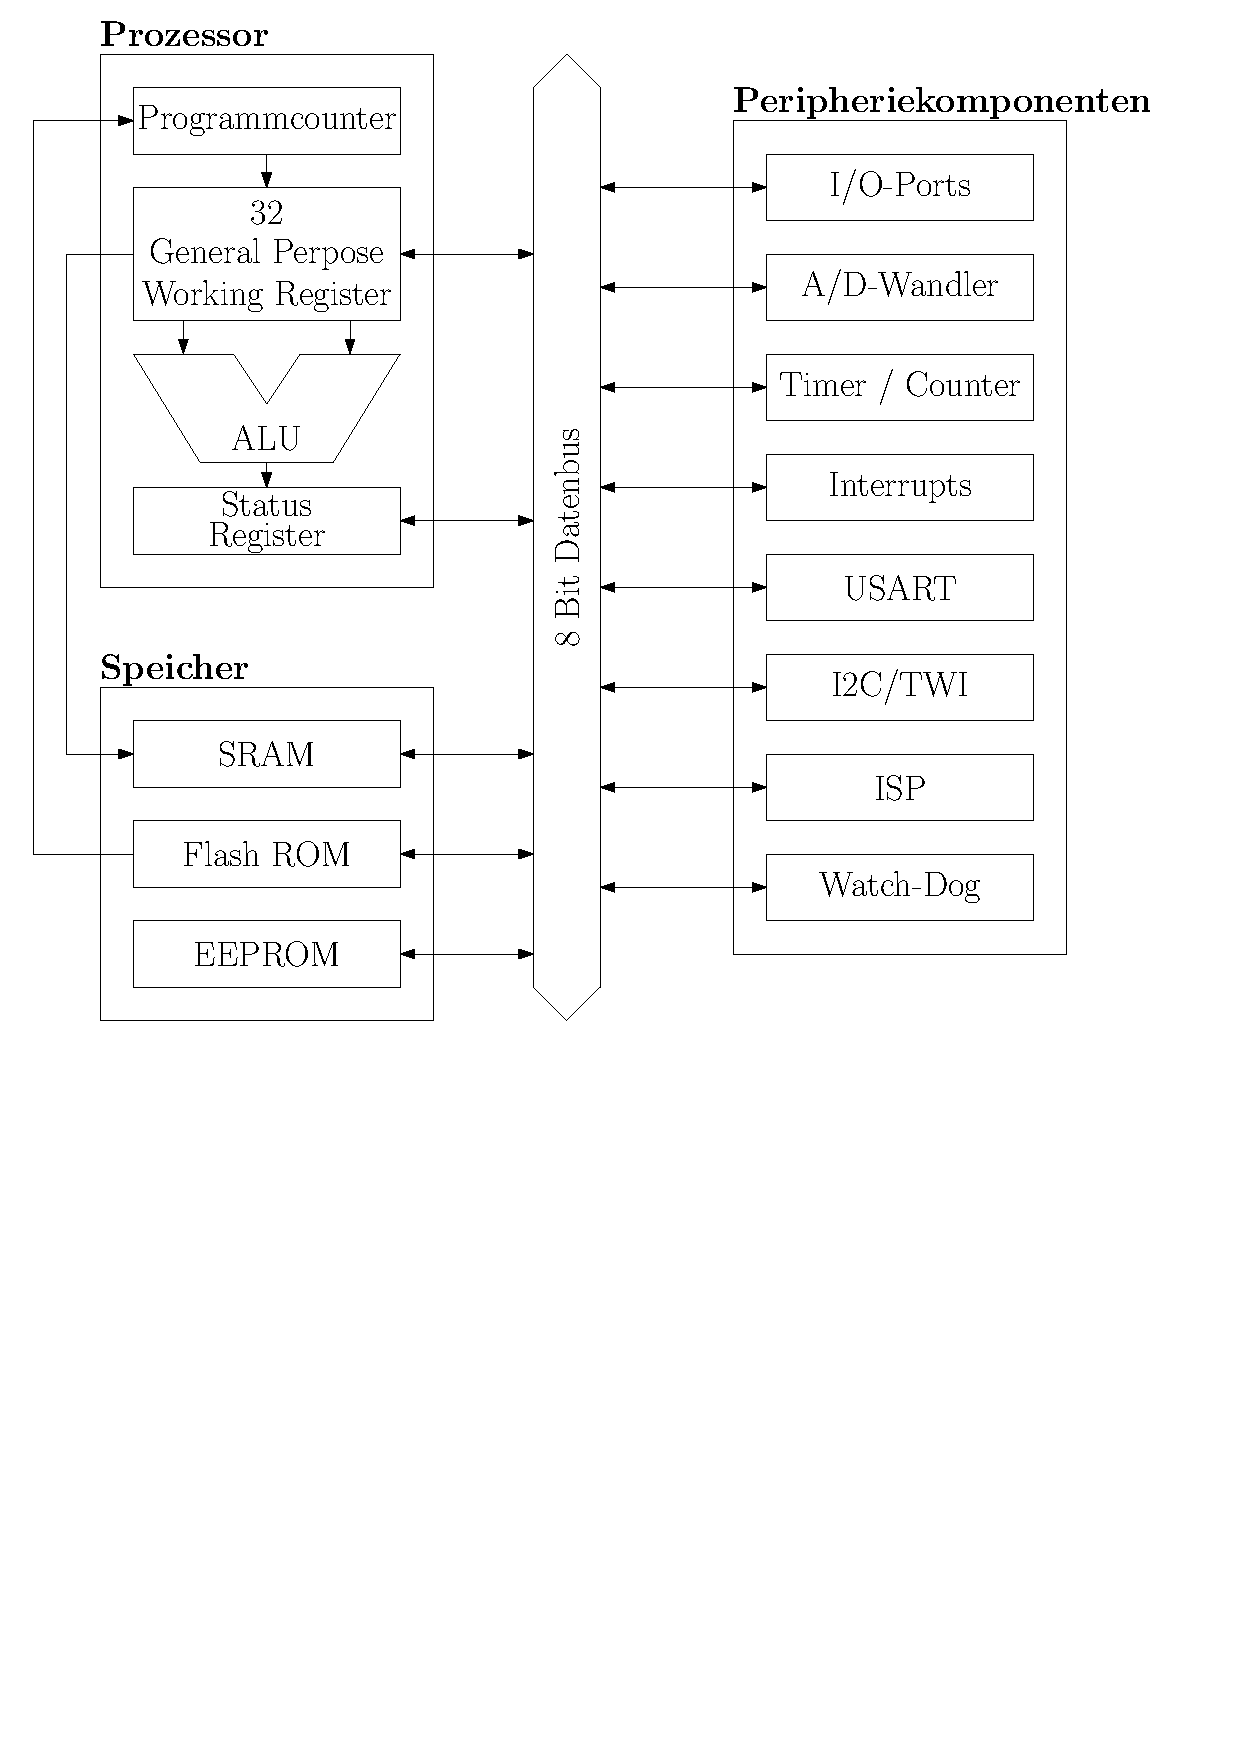
\includegraphics[width=0.8\textwidth]{flow/schemamc.pdf}
	\caption{Schematischer Aufbau eines Mikrocontrollers vgl. \cite{Brinkschulte:2002:Mikrocontroller}}
	\label{fig:aufbmc}
\end{figure}

Die zentrale Steuereinheit eines MCs ist der \textbf{Prozessor} (engl.: Central Processing Unit (CPU)). Sie ist die wichtigste Funktionseinheit und für die Verarbeitung von Befehlen und arithmetischen Berechnungen verantwortlich. Über den internen Bus kann die CPU mit weiteren Grundbausteien kommunizieren und beispielsweise auf Daten innerhalb des Speichers zugreifen.

Der \textbf{Speicher} besteht in der Regel aus dem Arbeitsspeicher (RAM, kurz für: Random Access Memory) und dem Programmspeicher bzw. Flash-Speicher. Normalerweise werden diese zwei Speichertypen logisch voneinander getrennt. Programme werden im nichtflüchtigen Flash-Speicher gesichert. Dieser kann mehrere Kilobyte (KB) bis Megabyte (MB) umfassen. Bei speziellen Systemen ist es möglich den Programmspeicher durch externe Flash-Komponenten zu erweitern um zusätzlichen Speicherplatz zu gewinnen.

Zwischenergebnisse, Messwerte von Sensoren, Steuergrößen usw. werden auf dem RAM abgelegt. Dieser ist deutlich schneller als der Flash-Speicher, verfügt aber in der Regel über deutlich weniger Speicherplatz. Alle Werte, welche zur Laufzeit im RAM abgelegt werden, sind im Gegensatz zum Flash-Speicher flüchtig. Das bedeutet, dass Daten bei einem Neustart des Mikrocontrollers nicht erhalten bleiben.

Durch die \textbf{Peripheriekomponenten} wird die Verbindung und Kommunikation zwischen Controller und Außenwelt ermöglicht. Über die digitalen Ein- und Ausgänge (GPIO, kurz für: General Purpose Input/Output) können Sensoren, Aktoren oder andere Systeme mit dem Mikrocontroller verbunden werden. Die meisten Mikrocontroller bieten eine Vielzahl von Ein- und Ausgängen \cite[S. 13-16]{SOM2012}.

Bei der Umsetzung des Projekts wurden \textsc{Mica}z-Module eingesetzt. Im Folgenden werden kurz die Eigenheiten dieser Module erläutert.

\paragraph{\textsc{Mica}z-Modul}
Ein \textsc{Mica}z-Modul ist drahtloser Sensornetzwerkknoten von der Firma Memsic. Mehrere dieser Module übernehmen in der physischen Zelle die Berechnung Geschäftslogik und die Steuerung der Rampen. \autoref{fig:micaz} zeigt ein solches Modul, während \autoref{fig:blockmicaz}  ein Blockdiagramm von dessen Struktur darstellt. Herzstück der Module ist ein ATMega128L-Mikrocontroller. Bei diesem handelt es sich um einen Low-Power-Mikrocontroller von der Firma Atmel. Darüber hinaus verfügt ein \textsc{Mica}z-Module über einen CC2420-Funkchip der Firma Texas Instruments. Dieser ermöglicht die drahtlose Kommunikation mit anderen Modulen auf einer Frequenz von 2.4 GHz ermöglicht. Es wird dabei der IEEE 802.15.4 Standard verwendet. Eine Antenne kann über eine MMCX-Schnittstelle mit dem Modul verbunden werden, um Signalstärke und -reichweite zu erhöhen. Weiter verfügen die Module über einen 128 KB großen Flash-Speicher.
Zugang zu einee Vielzahl der Leitungen des Moduls gewährt ein 51-poliger Steckverbinder. Über eine Erweiterungsplatine werden so etwa die Lichtschranken und Magnetbolzen der Rampe angeschlossen. Denkbar wäre auch ein größerer Arbeitsspeicher, alle nötigen Pins des Mikrocontrollers sind über den Steckverbinder erreichbar.
Im Projekt wurde die Steckverbindung weiterhin dafür genutzt, die \textsc{Mica}z-Module über ein \textsc{Mib}520 an einen PC anzuschließen, um sie über eine UART-Schnittstelle auszulesen und per JTAG (siehe \autoref{sec:JTAGICE3}) zu programmieren \cite{MICSHEET,C2420SHEET}.

\begin{figure}[th]
  \centering
    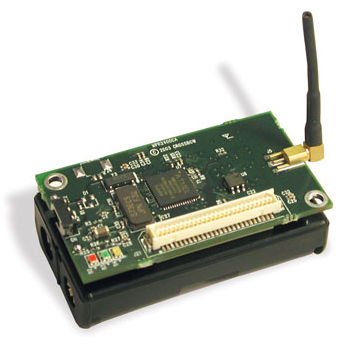
\includegraphics[width = 0.4\textwidth]{flow/micaz.png}
    \caption{\textsc{Mica}z-Modul \cite{Memsic:2014:Online}}
    \label{fig:micaz}
\end{figure}

\begin{figure}[th]
  \centering
    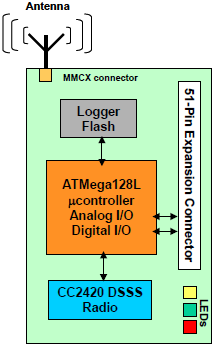
\includegraphics[width = 0.4\textwidth]{flow/blockmicaz.PNG}
    \caption{Blockdiagramm der \textsc{Mica}z-Module  \cite{Memsic:2014:Online}}
    \label{fig:blockmicaz}
\end{figure}

\paragraph{\textsc{Mib}520}
Ein \textsc{Mib}520 stellt eine Schnittstelle für \textsc{Mica}z-Module dar. Es erlaubt die Verbindung eines \textsc{Mica}z-Moduls mit einem Computer per USB-Schnittstelle. So kann über die USART-Schnittstelle des Moduls mit dem PC kommuniziert werden. Über diese Verbindung wurde die Schnittstelle zu den Volksbots realisiert. Weiterhin verfügt ein \textsc{Mib}520-Gateway über eine \textbf{JTAG}-Schnittstelle.


\subsection{Werkzeuge}

\subsubsection{Robot Operating System (ROS)}

Es gibt viele Robotik-Frameworks, die spezifisch für präzise Anwendungen, für Prototypen,
erstellt wurden. ROS strebt da eher das Allgemeine an. Das »Robot Operating System«
(ROS) ist ein Open-Source Framework für individuelle Roboter, das sich in der
Robotikforschung in den letzten Jahren etabliert hat und ein großes Repertoire an Software-Komponenten und -Werkzeugen für Robotikapplikationen bietet.\\
Die Entwicklung begann 2007 am Stanford Artificial Intelligence Laboratory im Rahmen des
Stanford-AI-Robot-Projektes (STAIR). Heute wird es hauptsächlich am Robotik Institut Willow
Garage weiterentwickelt. Seit April 2012 wird ROS von der neu gegründeten,
gemeinnützigen Organisation Open Source Robotics Foundation (OSRF) unterstützt. Die
Bibliotheken von ROS setzen auf Betriebssysteme wie Linux, Mac OS X oder Windows auf.
ROS ist nicht von einer spezifischen Sprache abhängig. Heutzutage gibt es 3 Grundlibraries
für ROS, die jeweils auf Python, Lisp und C++ ausgerichtet sind. Zwei Exmperimentier-
Librairies sind für Java und Lua erhältlich.
\subsubsection*{Was will ROS?}
\begin{itemize}
 \item ROS will unterstützen, Code für Forschung und Entwicklung wiederzuverwenden
 \item loser Verbund von individuellen Programmteilen (Nodes)
 \item einzelne Programmteile können einfach geteilt und verbreitet werden (Packages und Stacks)
 \item ROS stellt Repositories zu Verfügung, um dort Code zu teilen \cite{ROS:2014:Online}
(http://www.ros.org/browse)
\end{itemize}
\subsubsection*{Was kann ROS?}
Die Hauptbestandteile und Hauptaufgaben von ROS sind Hardwareabstraktion; Gerätetreiber; Implementierung 
von viel genutzten Funktionalitäten; Inter-Prozess-Kommunikation; Paket-Management
\subsubsection*{Aufgaben des ROS}
\begin{itemize}
 \item Interprozesskommunikation (IPC)
 \begin{itemize}
\item Problematik der Kommunikation zwischen verschiedenen Systemen des Roboters
\item Sicherheitseinstellung bei der Übertragung
\item Anforderung an die Geschwindigkeit / Schnelligkeit der Kommunikation
\item Koordination von Nachrichten durch zentralen Master
\end{itemize}
\item Paketverwaltung – Packages
\begin{itemize}
 \item ROS ist durch Softwarepakete (sogn. Packages) aufgebaut
 \item Ein Package beinhaltet Laufzeitprozesse (Nodes); ROS abhängige Bibliotheken;
Datensätze; Konfigurationsdateien;3rd Party Software
 \item Packages sind dazu, da um Code wiederverwendbar zu machen
\end{itemize}
\item Paketverwaltung – Stacks
\begin{itemize}
\item Sammlung von Paketen (Packages)
\item Der Sinn ist, dass Stacks die Verteilung und Verwendbarkeit von Code
vereinfachen
\item Meist viele Packages ähnlicher Aufgaben in einem Stack verpackt
\end{itemize}
\item Message (msg)
\begin{itemize}
 \item  Messages werden verwendet um unter ROS Nachrichten zwischen Knoten und
Topics auszutuaschen
\item Dafür verwendet ROS eine einfache Beschreibung der Datentypen in Textdateien
\item Durch diese Beschreibung kann für unterschiedliche Sprachen Code autogeneriert
werden
\item Diese sind in .msg-Dateien im msg- Unterverzeichnis eines ROS-Pakets abgelegt
\item Eigene Message-Typen sind mit Paket Ressource-Namen bezeichnet
\item Standard Messages sind mit std\_msg/msg/String.msg bezeichnet
\end{itemize}
\item Service
\begin{itemize}
 \item ROS verwendet eine eigene vereinfachte Service Description Language ("srv") für die
Beschreibung von ROS Service-Typen
\item Setzt direkt auf die ROS msg-Format auf
\item Ermöglicht die Anfrage / Antwort-Kommunikation zwischen den Knoten
\item Service-Beschreibungen sind in .srv-Dateien im srv- Unterverzeichnis eines Pakets
gespeichert
\item Service-Beschreibungen werden für die Verwendung mit dem Paket Ressource-
Namen bezeichnet
\item Z. B.: wird die Datei robot\_srvs/srv/SetJointCmd.srv als Service
robot\_srvs/SetJointCmd bezeichnet
\end{itemize}
\item Notes
\begin{itemize}
 \item Der Nachrichtenaustausch findet bei Nodes durch 3 Möglichkeiten statt: Parameter
Server;Topics; Services
\item Nodes werden wie in einem Graph angeordnet
\item In einem System laufen viele Nodes Parallel
\item Diese werden zu Beginn gestartet
\item Beispiele sind Nodes für: Laserscanner; Kinect; Pfadplanung
\end{itemize}
\item Topica
\begin{itemize}
 \item Topics verhalten sich wie ein virtuelles BUS-System Nodes können von Topics lesen
(subscribe)
\item Nodes können an Topics senden (publish)
\item Es gibt keine Begrenzung wie viele Nodes publsih oder subscribe auf ein Topic
machen
\end{itemize}
\end{itemize}
\subsubsection*{ROS-Datensystem}
ROS-Ressourcen sind in rangmäßiger Gliederung eingeordnet. Zwei Konzepte sind zu
verstehen:
\begin{itemize}
\item \textbf{Le package}: Es handelt sich hier um die Zentraleinheit der Softwareorganisation von
ROS. Ein Package ist ein Verzeichnis der die Knoten beinhaltet (wir werden hier
unten erklären, was ein Knoten ist) sowie die externen Librairies, Daten und XML
Konfigurationsdateien die manifest.xml genannt wird.
\item \textbf{Stack}: Stack bezeichnet eine Sammlung von Packagen. Sie ermöglicht mehrere
Funktionen wie Navigation, Lokalisierung und viele mehr. Ein Stack beinhaltet
mehrere Verzeichnisse sowie eine Konfigurationsdatei die stack.xml genannt wird.
\begin{itemize}
\item Vorhandene wichtige Stacks
\begin{itemize}
\item TF – Koordinatentransformation
\item Navigationstack
\item URDF - Modelle
\end{itemize}
\begin{itemize}
\item Beispiel Navigationstack
\begin{itemize}
\item Wertet Sensordaten aus z.B.: Laserdaten
\item Baut daraus mit gmapping (ebenfalls ein ROS-Stack) eine Begehbarkeitskarte
\item Warum? Zur Kollisionsvermeidung
\item Bei erfolgreicher Erstellung einer Map kann dann ein Ziel übergeben werde (Pfadplanung durch Navigationstack,
Kollisionsvermeidung, Reaktion auf sich ändernde Umgebung, Aufbau einer globalen Karte)
\end{itemize}
\end{itemize}
\end{itemize}
\end{itemize}
\subsubsection*{Vorteile und Nachteile des ROS}
\paragraph*{Vorteile}
\begin{itemize}
 \item Nachrichten-basierte Software Architektur
\begin{itemize}
\item Verschiedene Komponenten sind unabhängig voneinander mit dem System verbunden
\item Unterschiedliche Komponenten können miteinander verbunden werden, ohne jedes Mal das Programm neu zu Kompilieren
\item Netzwerkfähigkeit
\item Einfaches Debugging und Simulieren
\end{itemize}
\item Absturz eines Nodes führt nicht zum Absturz des ganzen
Systems
\item Für ROS lässt sich in mehreren Sprachen programmieren
\item ROS hat eine große Community, die viele Daten und Programme zu Verfügung
stellen
\end{itemize}
\paragraph*{Nachteile}
\begin{itemize}
 \item Durch Nachrichten-basierte Systemarchitektur Bottleneck bei großer Datenmenge
\item Steuerung des Systems über Kommandozeile
\end{itemize}

\subsubsection{Epos Control}

\subsubsection{SOPAS Engineeringtool}

Bei SOPAS ET handelt es sich um ein Entwicklungsprogramm von Sick. Dieses wird zur Ansteuerung und Konfiguration der Laserscanner und Hallsensosren verwendet.

\begin{itemize}
\item \textbf{ Erster Start }

Beim ausführen von SOPAS wird ein neues Projekt erstellt, in dem man die gewünschte Hardware selektiert und einbindet. Die Wahl der Hardware erfolgt hierbei über den Netzwerkscanassistenten oder manuell über den Gerätekatalog. Sobald die Kommunikation mit der Hardware aktiv ist, kann diese angesteuert werden. Änderungen der Konfiguration der Hardware sind im Projektbaum möglich oder sogar notwendig ( siehe Kapitel 7.7 Herausforderungen).
\end{itemize}


\subsection{Architektur}

Der systematische Aufbau des Volksbots ist in Abbildung \ref{fig:architecture_volksbot} dargestellt. Die Funktionen des Roboters basieren auf der Auswertung und Ansteuerung der Sensoren bzw. Aktoren. Alle Operationen, wie z.B. die Lokalisation, die Routenplanung, der Vorgang der Paketübergabe, laufen auf dem Robot Operating System und nutzen die Daten der Sensorik zur geeigneten Ansteuerung der Aktoren. Gesteuert werden die Operationen über die externe Kommunikationsebene, welche aus einem MICAz-Modul besteht. Hier werden Aufträge empfangen und auf der Operationsebene in zugehörige Ziele übersetzt.

\begin{figure}[h!]
 \centering
		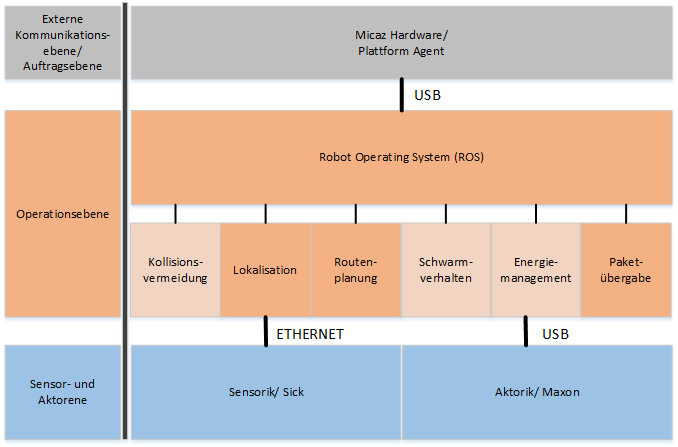
\includegraphics[width=1\textwidth]{drive/DRIVE_Architektur.png}
	\caption{Architektur des Volksbot}
	\label{fig:architecture_volksbot}
\end{figure}

Die in dunkleren rot hervorgehobenen Funktionen der Operationsebene deuten deren höhere Wichtigkeit an und geben ein erstes Anzeichen darauf welche Funktionen erfolgreich umgesetzt werden konnten.

\section{Implementierung}

Der erste Teil der Implementierung sah die Bereitstellung von Treibern für die komplette Hardware des Volksbots vor. Die Initialisierung und Ansteuerung der an den EPOS2-Controllern angeschlossenen Peripherie erfolgte unter der Verwendung der EPOS2 Bibliothek. Diese Bibliothek verfügt über alle benötigten Funktionen zum Ansteuern und Auslesen der Motoren und Lichtschranken, welche mit den EPOS-Controllern verbunden sind. Die Funktionen wurden dem ROS-Package „epos2-control“ zusammengeführt und sind in der Epos2MotorController-Node des Packages enthalten. 
Die Verwendung der Laserscanner, welche nicht mit den EPOS2-Controllern verbunden sind, wurde durch die Implementierung und Parametrisierung von im ROS vorhandenen Treibern gewährleistet. Dem an der Front des Roboters angebrachten SICK LMS100 Laserscanner, wurde dafür unter Windows eine feste IP-Adresse zugeordnet. Mit Hilfe dieser bekannten Adresse, konnte auch unter Ubuntu die Verbindung über Ethernet mit dem Laserscanner durch das Package „LMS1xx“  hergestellt werden.


\subsubsection{Implementierung der Navigation}
Nach erfolgreicher Inbetriebnahme der Hardware des Volksbots wurde die Odometrieberechnung anhand der zurückgelegten Strecke der Räder implementiert. Die Berechnung der zurückgelegten Wegstrecke und der Drehung des Roboters erfolgt über folgende Formeln\cite[S. 1]{Der:2000}:

\begin{equation}
\triangle s = \dfrac{\triangle R + \triangle L}{2}
\end{equation}
 
\begin{equation}
\triangle \alpha = \dfrac{\triangle R - \triangle L}{D}
\end{equation} 

Die Daten der Wegstrecke und der Drehung des Roboters werden genutzt, um mit folgenden Formeln die x- und y-Position des Roboters zu berechnen:

\begin{equation}
x = x(t-1) + (\triangle s * \cos (\alpha (t-1) + \triangle \alpha))
\end{equation} 

\begin{equation}
y = y(t-1) + (\triangle s * \sin (\alpha (t-1) + \triangle \alpha))
\end{equation} 

Der Drehwinkel des Roboters ergibt sich aus der Addition des vorherigen Winkels mit der zuletzt durchgeführten Änderung des Drehwinkels.

\lstinputlisting[language=C++, style=customc, captionpos=b, caption={Implementation der Odometrieberechnung}, label=lst:odom]{src/drive/lst/Odometrie.cpp}

Die Daten der Odometrie werden zur Lokalisierung des Roboters innerhalb einer mit dem SICK LMS100 Laserscanners erstellten Umgebungskarte verwendet. Die Implementierung erfolgte ebenso wie bei der Entwicklung der Treiber im „epos2-control“-Package. Bei der Erstellung der Umgebungskarte wurde auf das „Gmapping“-Package von ROS zurückgegriffen. Der darin enthaltene Algorithmus nutzt die Daten des Laserscanners, um während der Fahrt des Roboters aus seiner erfassten Umgebung eine Karte zu erstellen. Zur Visualisierung der Karte und der Daten des Laserscans wurde „Rviz“, ein Visualisierungstool innerhalb der ROS-Umgebung verwendet. Mit Hilfe von Rviz ist es neben der Visualisierung unter anderem möglich die initiale Position des Roboters, sowie Navigationsziele innerhalb der Karte festzulegen. (Screenshot Rviz) Mit dem Ziel den auftretenden Abweichungen der Odometrieberechnung entgegenzuwirken, wurde das „adaptive Monte Carlo Localisation“-Package (AMCL) implementiert. Vereinfacht formuliert, nutzt dieses Verfahren die Daten des Laserscans und der Karte, um mit Hilfe der Merkmale des aktuellen Scans und der zugrundeliegenden Daten der Kartenrepräsentation eine Schätzung der Position des Roboters auszuführen. \cite[S. 6]{Bischoff:2004}
Eine funktionsfähige Selbstlokalisation ist die Grundlage für eine erfolgreiche autonome Navigation in der Umgebung des Roboters. Das ROS-Framework stellt mit dem „move-base“-Package die nötigen Funktionen für die Navigation bereit. Das Package hat den Dijkstra-Algorithmus zur Wegplanung implementiert und nutzt zwei parametrisierbare Costmaps, um Eigenschaften wie z.B. den Mindestabstand zu Hindernissen oder das Verhalten bei Planungsfehlern festzulegen. Nach der Planung des Weges werden automatisch die passenden Steuerbefehle generiert. Falls der Volksbot in eine unvorhergesehene Situation gerät und seine geplante Route nicht mehr gültig ist, kommen Rettungs-Funktionen des Packages zum Einsatz. Dabei wird eine Rotation um die eigene Achse des Roboters durchgeführt, um einen geeigneten neuen Weg zu finden. 

\subsubsection{Implementierung der Paketübergabe}
Damit der Austausch der Pakete mit den Komponenten des Materialflusses erfolgen kann, musste die Kommunikation über die MICAz-Module und Automatismen zur Anpassung der Hub-Position an die Höhe der jeweiligen Rampe implementiert werden. Nachdem ein Auftrag vom Materialfluss empfangen wurde, wird die Annahme des Auftrags dem Materialfluss bestätigt und der Auftrag  in ein passendes Navigationsziel auf der Umgebungskarte umgesetzt.  Für den Prozess des Entschlüsselns von den Nachrichten des Materialflusses wurde ein ROS-Package namens „Simple-Navigation-Goals“ implementiert. Neben der Umsetzung von Navigationszielen sendet dieses Package ROS-interne Nachrichten, welche Informationen über die gewünschte Position des Hubs und das Erreichen der Zielposition enthalten.
Sobald die Zielposition erreicht wurde, beginnt die Hubsteuerung mit der Anpassung der Hubposition an die geforderte Höhe. Anschließend folgt eine Benachrichtigung an den Materialfluss und das Förderband wird in Gang gebracht. Die Auswertung der Lichtschranken bewirkt den Haltevorgang des Förderbands und das nächste Navigationsziel wird festgelegt.

\subsubsection{Struktur der einzelnen Funktionalitäten}



\begin{figure}[h!]
 \centering
		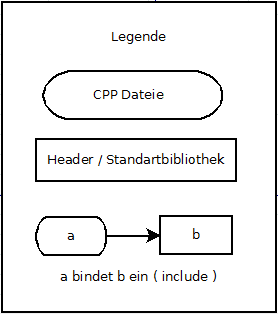
\includegraphics[width=0.4\textwidth]{drive/Legende.png}
	\caption{Legende zu Abb. 46 und 47}
	\label{fig:Legende}
\end{figure}

\begin{figure}[h!]
 \centering
		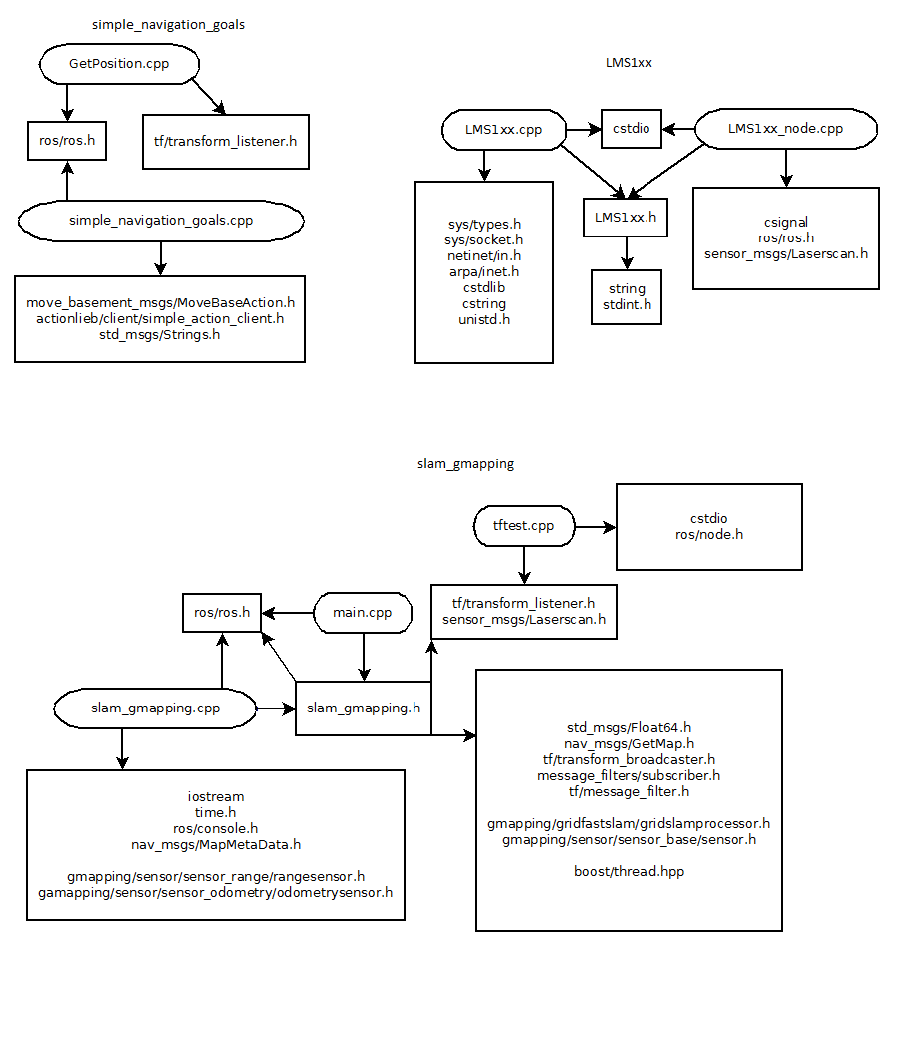
\includegraphics[width=1\textwidth]{drive/funktionen.png}
	\caption{eingebundene Funktionen in ROS}
	\label{fig:funktionen}
\end{figure}

\begin{figure}[h!]
 \centering
		\includegraphics[width=1\textwidth]{drive/epos2_control.png}
	\caption{Hauptsteuerung des Systems ( Epos2 Control )}
	\label{fig:epos2_control}
\end{figure}


\input{src/drive/6_Funktionalitäten}

\subsection{Herausforderungen}

Bei der Implementierung der Funktionen des Volksbot traten einige Herausforderungen auf, deren Lösungen besonderen Aufwand hervorriefen oder nicht umgesetzt wurden. Ein Beispiel dafür ist die Selbstlokalisation des Roboters durch die Odometrieberechnung und dessen Verbesserung durch die adaptive Monte Carlo Lokalisation (AMCL). Aufgrund der Fehleranfälligkeit der einfachen Odometrie durch Einflüsse wie z.B. die Beschaffenheit des Bodens ist der Einsatz von Algorithmen wie die adaptive Monte Carlo Lokalisation, welcher die Daten des Laserscanners nutzt, notwendig.  Die Qualität der Odometrie musste durch das Kalibrieren des Parameters der Achsenlänge des Roboters erhöht werden, um die nötige Voraussetzung für einen funktionierenden AMCL-Algorithmus zu schaffen. Eine gute Odometrie lässt sich dadurch erkennen, dass die Punkte des Laserscans auch bei Bewegung weiterhin mit den Wänden der Umgebungskarte übereinstimmen. Getestet wurde die Odometrie durch die verzögerte Darstellung der Laserscans in Rviz bei der Drehung des Roboters. Die Laserscan-Punkte würden bei einer guten Odometrie den Raum relativ genau nachzeichnen und die Laserpunkte würden sich überlappen. Ein Vergleich zwischen einer guten Odometrie-Einstellung (links) und einer schlechten (rechts) ist in Abbildung \ref{fig:Odo_vergleich} dargestellt.

\begin{figure}[h!]
 \centering
		\includegraphics[width=1\textwidth]{drive/Odometrie_vergleich.png}
	\caption{Vergleich von Odometrie-Einstellungen mit Hilfe von verzögert dargestellten Laserscan-Punkten}
	\label{fig:Odo_vergleich}
\end{figure}

Bei der Parametrisierung der Wegplanung musste ein Gleichgewicht zwischen Geschwindigkeit und Genauigkeit gefunden werden, um ein stabiles System zu schaffen. Durch die Vielzahl der Möglichkeiten war die Suche nach geeigneten Einstellungen problematisch. Ein Beispiel dafür ist die Parametrisierung der Zieltoleranzen. Einerseits hat die Verringerung der Zieltoleranzen bewirkt, dass sich der Roboter der Zielposition exakter nähert. Andererseits dauert die Ausrichtung des Roboters deutlich länger, da der Roboter mehrere Rotationen ausführt bis die geeignete Position erreicht wurde. Letztlich wurde eine genauere Positionstreue des Roboters priorisiert, um die Fehleranfälligkeit bei der Paketübergabe zu senken.

Eine weitere Herausforderung stellte die Erkennung von Hindernissen dar, die ober- oder unterhalb des Laserscanners in den Raum ragen. Zur Lösung dieses Problems könnte ein weiterer bildgebender Sensor genutzt werden, um den gesamten Raum nach potenziellen Hindernissen zu untersuchen oder eine Anpassung der Arbeitsumgebung durchgeführt werden.

Mit großem Aufwand war die korrekte Ansteuerung der Maxon Controller verbunden. Besonders die Parametrisierung des kleineren Maxon Controllers unter ROS, welcher für den Betrieb des Förderbandes verwendet wird, stellte sich als Problem heraus. Schon kleinere Abweichungen der Parameter für Spannungs- und Beschleunigungswerte in der Ansteuerung des Controllers führten zu Systemabstürzen.
 
Die Programmierung und Parametrisierung der Teilfunktionen musste mit Blick auf
die CPU-Auslastung der Steuereinheit geschehen, da einige Berechnungen bei falscher
Verwendung zu sehr hohen Auslastungen und einer unzureichenden Performance des
Roboters führten. Ein Beispiel dafür ist die Funktion zur Kommunikation mit Hilfe des MICAz-Moduls, welche     regelmäßig unterbrochen werden musste.

Ein weiteres Problem stellte der LMS 100 Laserscanner von SICK dar. Dieser wird mittels Ethernet-Anschluss mit der Steuereinheit verbunden und sollte mittels seiner IP Adresse durch ROS direkt verwendet werden können. Allerdings konnte weder ROS noch SOPAS ET ( siehe Kapitel 3..3.3 ) auf den Scanner zugreifen. Beim erstellen eines Projekts in SOPAS war der Netzwerkscanassistent nicht in der Lage den Laserscanner zu erkennen und somit musste der LMS 100 manuell im Gerätekatalog ausgewählt und in das Projekt eingebunden werden. Bei der Verbindung zum LMS 100 wurde die bestehende IP Adresse des Scanners angezeigt und eine Neuzuweisung einer IP Adresse angeboten. Die Neuzuweisung der IP Adresse ist notwending, damit ROS eine Verbindung zum LMS 100 herstellen konnte.

\subsection{Ausblick}

Der Volksbot sollte um folgende Funktionalitäten erweitert werden:

\begin{itemize}

\item \textbf{Genauigkeit bei der Übergabe}: Die Genauigkeit des Heranfahrens an eine Zielposition, wie z.B. den Ausgang einer Rampe, muss verbessert werden, um eine erfolgreiche Übergabe zu gewährleisten. Durch die Fehleranfälligkeit der Odometrie sollte eine alternative Prozedur zur Ansteuerung der Rampen entwickelt werden, um die Paketübergabe mit höherer Erfolgswahrscheinlichkeit zu realisieren.

\item \textbf{Kollisionserkennung mobile Hindernisse - Schwarmverhalten}: Der Volksbot sollte Hindernisse, die sich selbstständig bewegen, erkennen und entsprechend reagieren. Dies könnte beim erkennen eines Objektes mittels einer Neuplanung der Route, einer kurzen Unterbrechung der Fahrt oder eines Ausweichmanövers umgesetzt werden. Besonders bei der Verwendung von mehreren Volksbots sollte eine Funktion zur Bahnreservierung implementiert werden. 

\item \textbf{Rückkopplung an Simulation}: Die Volksbots sollten ihre aktuelle Position, sowie den Beladungs- und Energiezustand an die Simulation zurückgeben.

\item \textbf{Fahralgorithmus}: Es können alternative Algorithmen implementiert werden, um die Berechnungszeiten zu verkürzen oder optimale Routen zu finden.

\item \textbf{Kostenabschätzung}: Eine optimale Berechnung zur Bestimmung der benötigten Zeit, Strecke und Energieverbrauchs würde die Jobverteilung effizienter gestalten.

\item \textbf{Ladestation}: Die Ladestation muss angebracht und getestet werde. Danach fehlt die automatische Erkennung des kritischen Zustandes, sowie das selbstständige anfahren der Ladestation, damit der Akku geladen werden kann. Hierbei handelt es sich um einen Prototypen der noch getestet werden muss.

\end{itemize}




















	
	% Chapter Integration
	\clearpage
	\ohead[Integration]{Integration}
	\chead[Uni Oldenburg]{Uni Oldenburg}
	\ihead[PG FAISE]{PG FAISE}
	\setheadtopline{1pt}
	\setheadsepline{0.5pt}
	\ofoot[Endbericht]{Endbericht}
	\cfoot[\pagemark]{\pagemark}
	\ifoot[30. September 2014]{30. September 2014}
	\setfootsepline{0.5pt}
	\setfootbotline{1pt}
	\section{Integration der Teilsysteme}
Nachdem in den vorigen Abschnitten die jeweiligen Teilsysteme eingehend besprochen und vorgestellt wurden, wird in diesem Kapitel nun deren Integration beschrieben.

Dafür wird zunächst auf die fertiggestellte physische Zelle und auf deren Struktur und Verhalten eingegangen. Im nächsten Schritt werden dann die bereits erfolgten und die aus unserer Sicht nötigen Maßnahmen für eine vollständige Integration von Simulation und physischer Zelle beschrieben. Abschließend werden die Besonderheiten in der Implementierung der Teilsysteme erläutert, die bei der zukünftigen beziehungsweise weiteren Umsetzung dieser Integration von Bedeutung sind.
 
\subsection{Die physische Zelle}

\subsubsection{Aufbau}
\subsubsection{Ablauf}

Im folgenden wird der Ablauf für einen Transport innerhalb des physikalischen Aufbau aus Abbildung \ref{fig:physischeZelle} vom Ausgang der Rampe A zum Eingang der Rampe B beschrieben. Dafür muss zunächst ein Paket in das System initialisiert und dadurch ein Auftrag generiert werden. Anschließend kann durch den Materialfluss der Transport ausgelöst werden.

\begin{itemize}
\item Volksbot wird lokalisiert und wartet auf Auftrag
\item Registrierung der Pakete im System (Gateway)
\item Materialfluss sendet Nachricht (Opcode mit Ziel-ID: Ausgang Rampe A) an Volksbot
\item Volksbot entschlüsselt Opcode und startet Navigation zu Rampe A
\item Hubposition am Volksbot wird auf Höhe Ausgang Rampe A gefahren
\item Wenn Volksbot Navigationsziel erreicht hat und Hubhöhe eingestellt ist, wird eine Statusrückmeldung an Materialfluss gesendet
\item Rampe A gibt das Paket ab und der Volksbot nimmt durch Ansteuerung der Floweinheit das Paket auf
\item Volksbot fährt zum Eingang Rampe B und regelt die Hubhöhe auf entsprechende Rampenhöhe
\item Volksbot gibt Statusrückmeldung an Materialfluss und löst Paketübergabe aus
\item Volksbot frei für nächsten Auftrag


\end{itemize}


\subsection{Integration von Simulation und physischer Zelle}
\label{sec:Hybrid}
Bezogen auf das Gesamtsystem bietet es sich an, das physische und das virtuelle Teilsystem mithilfe eines hybriden Modus miteinander zu verknüpfen. Ein solcher Hybridmodus bietet viele weitere Möglichkeiten und könnte auf unterschiedlichen Wegen realisiert werden. Beispielsweise könnte die Software das physische System steuern, indem generierte Aufträge an das reale System geschickt werden. Auch könnten die Aktionen der Fahrzeuge und Rampen in der Software visualisiert werden. Besteht ein Teil der Visualisierung aus der Darstellung der realen Akteure und der andere aus rein virtuellen Akteuren, so könnten physische und virtuelle Akteure ein Gesamtsystem bilden, dass die Skalierbarkeit des physischen Systems erhöht. Dies setzt jedoch voraus, dass die Akteure aus beiden Systemen in ihren Eigenschaften (Geschwindigkeit etc.) weitestgehend aneinander angeglichen sind. Die technischen Voraussetzungen für das einbringen und abhören von drahtlosen Nachrichten in der physischen Zelle sind bereits durch Gateways realisiert. Die einzelnen physischen Module (Volksbots, Rampen) müssten jedoch zusätzlich regelmäßig über ihren Zustand informieren, um eine sinnvolle Auswertung der physischen Zelle in der Simulationsoberfläche zu erlauben. Gleichzeitig muss in der Simulation eine Möglichkeit geschaffen werden, physische Module hinzuzufügen, die nicht vom System simuliert, sondern stattdessen über Agentennachrichten angesprochen werden und Auskunft über ihren Zustand geben.

\subsection{Plattformbedingte Besonderheiten}

\subsubsection{Multiagentensystem und dessen Laufzeitumgebung}
Sowohl im Teilsystem Simulation als auch im Materialfluss kommen Agenten zum Einsatz, die die Betriebslogik abbilden. 

Da beide jedoch auf sehr unterschiedlichen Plattformen (Webserver beziehungsweise verteilte Mikrocontroller) zum Einsatz kommen, kann kein einheitliches Multiagentensystem zum Einsatz kommen. Stattdessen wird in der Simulation JADE verwendet, während im Materialfluss ein eigens entwickeltes AgentRTE zum Einsatz kommt, das speziell für den Einsatz auf Mikrocontrollern angepasst wurde. Bedingt durch die zur Verfügung stehenden Ressourcen ist dieses System im Bezug auf die maximale Kommunikationsbandbreite, die maximale Anzahl an Agenten und die Anzahl der gepufferten Nachrichten deutlich eingeschränkter. Auch erlaubt es im Gegensatz zu JADE keine \textit{Behaviors}, sondern das Verhalten der Agenten muss prozedural oder mit Zustandsautomaten abgebildet werden.

Die ausgetauschten Agenten-Nachrichten hingegen sind in beiden Systemen zumindest an den FIPA-Standard angelehnt, eine Umwandlung von einem in das andere Format kann daher durch eine einfache Abbildung realisiert werden. Weiterhin ist im physischen System die genaue Reihenfolge der Nachrichten-Parameter von großer Bedeutung, da hier nicht mit Objekten, sondern mit Byte-Arrays gearbeitet wird, die entsprechend interpretiert werden.

Das Multiagentensystem, dass für die Simulationssoftware entwickelt wurde, enthält neben den vier "Standardagenten" noch einen Job- und Statistikagent (Vgl. Abschnitt 5.4.5). Der Statistikagent hat keinen Einfluss auf den Ablauf der Simulation, der Jobagent hingegen übernimmt die Verteilung von Paketen und ausgehenden Aufträgen. Bei der Integration beider Teilsysteme muss der Jobagent miteinbezogen werden, sofern Pakete vom physischen System zu den Eingängen des virtuellen Systems  gelangen. Ist dies der Fall, so muss der Jobagent in die Datenübertragung miteinbezogen werden, da Eingänge keine eigenen Mechanismen zur Paketannahme besitzen. werden lediglich Pakete aus der Simulation zum physischen System befördert, so muss der Jobagent nicht miteinbezogen werden. Jedoch gibt es noch keinen Mechanismus, um Pakete, die an Ausgangsrampen eintreffen, aus der Simulation zu entfernen. Bei einer Integration beider Systeme über die Ausgangsrampen, könnte ein solcher Mechanismus im Abgleich mit dem physischen System entwickelt werden. 
\\\\
Physisches System und virtuelles System unterscheiden sich hinsichtlich des Paketagenten. In der Simulation wurde ein Paketagent erstellt, der alle Pakete verwaltet anstatt eines Paketagenten für jedes Paket. Grund dafür war, dass die Vielzahl an Agenten, die auf Basis von Jade und alle auf derselben Maschine liefen, zu Performance- und Synchronisationsproblemen führten. Eine weitere Aufsplittung des Paketagenten hätte diese Probleme noch verschärft. Für die Integration der beiden Teilsysteme muss untersucht werden, welche Aufgaben des Orderagenten der Paketagent in der Simulation übernimmt. Damit die Kommunikation zwischen zwei Rampen aus jeweils einem Teilsystem funktioniert, müssen die Kommunikationsprozesse zwischen den Agenten ggf. angepasst werden. Es ist unter Umständen möglich, dass beispielsweise die Zielfindung zwischen zwei Rampen im physischen Teilsystem andere Agenten einbezieht als die Zielfindung zwischen zwei Rampen aus beiden Teilsystemen.
\subsubsection{Pathfinding des Volksbot und in der Simulation}

	
		% Chapter 9 Ergebnisse
	\clearpage
	\ohead[Ergebnisse]{Ergebnisse}
	\chead[Uni Oldenburg]{Uni Oldenburg}
	\ihead[PG FAISE]{PG FAISE}
	\setheadtopline{1pt}
	\setheadsepline{0.5pt}
	\ofoot[Endbericht]{Endbericht}
	\cfoot[\pagemark]{\pagemark}
	\ifoot[30. September 2014]{30. September 2014}
	\setfootsepline{0.5pt}
	\setfootbotline{1pt}
	\section{Ergebnisse}
Dieses Kapitel gibt einen abschließenden Überblick über die erreichten Ergebnisse der Projektgruppe. Zunächst sollen zusammenfassend beschrieben werden, welche Komponenten erfolgreich entwickelt wurden. Im Fazit werden die aus der Projektarbeit gewonnenen Erkenntnisse und Erfahrungen beschrieben. Der letzte Teil dieses Kapitels beinhaltet eine Vision, in der potenzielle Weiterentwicklungen und Ideen aufgegriffen werden. 

\subsection{Realisierte Ziele}

Die Teilgruppe Simulation hat ein Simulationstool erstellt, das als Webanwendung realisiert wurde. Das Tool erlaubt das Erstellen von Szenarien mit einer vom Nutzer festgelegten Anzahl von Fahrzeugen und Rampen. Auch kann ein Nutzer eine beliebige Anzahl an Aufträgen generieren, die als Input für das Simulieren eines Szenarios dienen. Die Aktionen der Akteure werden serverseitig durch das Multiagentenframework JADE realisiert und clientseitig dargestellt. Jeder Akteur wird durch mehrere Agenten realisiert, die Zielsuche und Suche eines Transportmittels autonom und ohne zentrale Steuerung durchführen. Die Agenten der Fahrzeuge sind in der Lage mit einem selbst erstellten Pathfinding-Algorithmus Routen zu berechnen und diese anschließend abzufahren. Für einen Simulationsdurchlauf werden Daten über Paketdurchlaufzeit und Auslastung der Roboter mitgeloggt, die in der Statistik eingesehen werden können.

Die Teilgruppe Materialfluss hat während der Projektarbeit ein lauffähiges System für den Materialfluss auf Agentenbasis fertiggestellt. Zunächst wurde dafür ein vollständiges Agenten-System auf den unterschiedlichen Modulen umgesetzt. Es erlaubt die parallele Arbeit von bis zu sieben Agenten pro \textsc{Mica}z-Modul und den Austausch von Agenten-Nachrichten sowohl innerhalb eines Moduls als auch modulübergreifend. So ermöglicht es die Überwachung und Lokalisierung aller Rampen und Pakete, die sich im System befinden. Ein am Eingang liegendes Paket kann durch das System bis zu einem gewünschten Ausgang geleitet werden. Dazu gehört zum einen, dass die Module untereinander über ihre Funkschnittstelle kommunizieren können. Es wurde außerdem die Kommunikation zwischen den \textsc{Mica}z-Modulen und Volksbots über ein definiertes Kommunikationsprotokoll erfolgreich umgesetzt. Ein weiteres Merkmal in der Funktionalität ist das gelungene Zusammenspiel zwischen Rampen und Modulen, also die Abfrage und die Ansteuerung von Sensorik und Aktorik. Dies erlaubt die Vereinzelung von Paketen durch gezieltes öffnen und schließen der Bolzen. Außerdem wird die Überwachung der einzelnen Rampenplätze durch die angebrachten Lichtschranken ermöglicht. Eine weitere erfolgreich umgesetzte Funktionalität, ist die Möglichkeit Pakete durch das System routen zu lassen. Dabei wird ein verteiltes Protokoll auf Basis von kommunizierenden Zustandsautomaten mit plattformübergreifender Kommunikation der Agenten eingesetzt.

Die Teilgruppe Fahrzeuge hat einen autonom agierenden Pakettransport auf Basis des Volksbot zwischen den Rampen realisiert. Die Funktionen auf dem Volksbot sind in drei Bereiche zu unterteilen. Zunächst wurde mithilfe des Laserscanner und AMCL für eine erfolgreiche Navigation und Lokalisation gesorgt. Als weiteres Funktionspaket konnte die Paketübergabe realisiert werden. Der Volksbot ist in der Lage nach erreichen einer Rampe eine Paketübergabe durch Ansteuerung der Flow- und Hubaktoren durchzuführen. Für die Statusrückmeldung und das Empfangen von Aufträgen wurde eine Kommunikationsschnittstelle zwischen Volksbot und Materialfluss durch MICAz Controller realisiert. Im Ganzen kann sich der Volksbot autonom innerhalb der physischen Zelle navigieren, Aufträge entgegennehmen und ausführen.

Insgesamt konnte durch die Integration der Volksbots in den Materialfluss ein einfaches Umschlaglager innerhalb der physischen Zelle abgebildet werden. 



\subsection{Fazit}
Im Rahmen der Projektgruppe wurde von zwölf Teilnehmern ein System entwickelt, dass auf die drei Teilgruppen Materialfluss, Fahrzeuge und Simulation verteilt wurde. Durch die gemeinsame Arbeit an einem Projekt konnten Erfahrungen und Erkenntnisse auf dem Gebiet der Projektarbeit und Softwareentwicklung gewonnen werden. Ein wesentlicher Erfolgsfaktor eines Projekts ist das effektive Nutzen der vorhanden Zeit bei einem Projekt mit begrenzter Dauer. Grundsätzlich wurden Aufgaben sorgfältig und möglichst schnell durchgeführt. Für zukünftige Projekte empfiehlt es sich jedoch das Zeitmanagement zu optimieren, indem versucht wird Aufgaben noch weiter zu parallelisieren. Im Rahmen der Anforderungserhebung hatte sich bereits herausgestellt, dass bestimmte Technologien, wie beispielsweise ein Multiagentensystem zu einem späteren Zeitpunkt benötigt werden. Die Einarbeitung in benötigte Technologien erfolgte jeweils kurz vor der Implementierung einer Technologie, wodurch sich die Entwicklungszeit verlängerte. Um die Entwicklungszeit zu verkürzen, sollten Teilnehmer eines Projekts sich vor der Implementierung einer Komponente in die benötigte Technologie einarbeiten und diese für die anderen Teilnehmer aufbereiten. 
\\\\
Die Durchführung des Projekts mithilfe des Scrum Vorgehensmodell beinhaltete Sitzungen mit den Auftraggebern in denen die festgelegten Anforderungen mit den tatsächlich realisierten abgeglichen wurden. So konnten Eigenschaften des Produkts, die nicht den Vorstellungen der Auftraggeber entsprachen, direkt und mit geringerem Aufwand korrigiert werden. Ein solcher Abgleich sollte unabhängig vom dem gewählten Vorgehensmodell regelmäßiger Bestandteil eines Projekts sein. 
 

\subsection{Vision}
Für die Simulationssoftware bieten sich folgende Optimierungsmöglichkeiten: Die Fahrzeuge fahren selbstständig zu einem Ziel ohne dabei Kollisionen mit anderen Fahrzeugen zu vermeiden. Die Fahrzeuge fahren durcheinander durch. Um Kollisionen vorzubeugen, könnten Pfade entweder reserviert werden oder Roboter könnten untereinander Nachrichten austauschen, um festzustellen, ob ein Feld frei ist oder nicht. Um den Kommunikationsaufwand zu verringern, empfiehlt es sich Pfade zu reservieren. Weiterhin sollte es die Möglichkeit geben Roboter zur Laufzeit hinzuzufügen, da ein physisches System auch dynamisch skaliert werden kann, indem ein weiterer Roboter hinzugefügt wird. Durch den Einbau der beschriebenen Features erweitern sich die Möglichkeiten des Tools und die Ergebnisse eines Durchlaufs sind aussagekräftiger.
\\\\
Für die Implementierung der Agenten wurde JADE ausgewählt. JADE ermöglicht es Agenten in Echtzeit miteinander kommunizieren zu lassen. Das ebenfalls javabasierte MASON Framework, das von der George Mason Universität aus den U.S.A entwickelt wurde, bietet keine Echtzeitkommunikation, sondern steuert alle Agenten mit einem Scheduler. Der Scheduler unterteilt eine Simulation in verschiedene diskrete Schritte und führt bei jedem Schritt alle Agenten aus, die an der Reihe sind. Ein solcher Scheduler bietet den Vorteil, dass Scheduling Probleme reduziert werden können. Jedoch stellt sich die Frage, ob man einen Simulationslauf weiterhin in Echtzeit laufen lassen kann bzw. Echtzeit simulieren kann, wenn man ein Framework nutzt, dass einen Scheduler beinhaltet. Für zukünftige Modifikationen stellt sich die Frage, welche Möglichkeiten sich durch die Nutzung eines Schedulers ergeben.
\\\\
Im Materialfluss sollten im nächsten Schritt auch Zwischenlager-Rampen in das Routing der Pakete einbezogen werden. So könnte etwa berechnet werden, ob es kostengünstiger ist, ein Paket vom Eingang zum Ausgang über eine Zwischenrampe zu liefern oder nicht. Außerdem können Pakete, denen noch kein Ziel im System zugewiesen wurde, hier zwischengelagert werden, um Ein- und Ausgangs-Rampen nicht unnötigerweise zu blockieren.

Das Routing kann noch weiter ausgebaut werden, indem Zeitslots und Reservierungen auf Plattformen eingeführt werden werden. So können die Durchlaufzeiten der Pakete und die Gefahr von Deadlocks verringert werden.

Es ist zudem möglich, den Materialfluss auf existierende Stetigförderer auszuweiten. Für diese muss das AgentenRTE teilweise angepasst und es müssen dedizierte Plattformagenten für jeden Stetigförderer entwickelt werden. So kann das Gesamtsystem deutlich erweitert werden: Durch die Möglichkeit der Stetigförderer, mehrere Pakete in unterschiedlichen Richtungen auszugeben, werden Durchsatz und Flexibilität deutlich erhöht.
\\\\
Innerhalb der Fahrzeuge sollte in einem nächsten Schritt noch weitere Funktionalitäten implementiert werden.

Bieten: Der Volksbot sollte in der Lage sein an einer Auftragsverteilung teilzunehmen, sofern er noch keinen Auftrag ausführt und sein Energievorrat nicht das kritische Minimum erreicht hat. Die Teilnahme beinhaltet eine Aufwandsschätzung anhand einer Distanzfunktion, sowie dem aktuellen Energiezustand. 

Energiemanagement: Sobald ein Volksbot seinen kritischen Energiezustand erreicht, werden alle Auftragsverteilungen ignoriert und der Bot setzt die Dockingstation als primäres Ziel. Sollten mehrere Bots die Ladestation ansteuern, oder diese bereits belegt sein, so wird der Folgeablauf durch eine Queue oder ein anderes Verfahren geregelt.

Kollisionsvermeidung: Sobald eine Kollision mit einem festen oder mobilen Objekt erkannt wird, wird eine Neuberechnung, Umplanung oder ein Ausweichverfahren eingeleitet um entsprechend zu reagieren. Die Kollisionsvermeidung reagiert dynamisch und reicht weiter als die Auslösung eines Notstopps. Bei Verwendung von mehreren Volksbots wird eine Bahnplanung mit Reservierungsfunktion realisiert.
\\\\
Ein großer Teil der Vision betrifft weiterhin die bereits in \autoref{sec:Hybrid} genannte Integration von physischer Zelle und Integration. Die technischen Voraussetzungen für eine Kommunikation mittels eines Gateways sind bereits getroffen, deren Nutzung muss jedoch in allen Teilsystemen noch implementiert und aufeinander abgestimmt werden.
	
	% Bibliography
	\clearpage
	\clearscrheadfoot
	\ohead[Inhaltsverzeichnis]{Inhaltsverzeichnis}
	\chead[Uni Oldenburg]{Uni Oldenburg}
	\ihead[Malte Falk]{Malte Falk}
	\ofoot[Seminararbeit]{Seminararbeit}
	\cfoot[\pagemark]{\pagemark}
	\ifoot[WS 2013/14]{WS 2013/14}
	\ohead[Literaturverzeichnis]{Literaturverzeichnis}
	\printbibliography

\end{document}
